	% !TEX TS-program = XeLaTeX
% اگر قصد نوشتن رساله دکتری را دارید، در خط زیر، گزینه msc را پاک کنید. کلیه تنظیمات لازم به طور خودکار اعمال می‌شود.
% در صورت استفاده از گزینه withpage  شماره صفحات حاوی نمادها در جلوی آن‌ها در فهرست نمادها چاپ می‌شود و در صورت 
% استفاده از گزینه printonlyused  فقط نمادهایی که در متن استفاده شده‌اند، در فهرست نمادها چاپ می‌شوند.
\documentclass[msc,withpage,printonlyused,fontsize=13pt]{yazd-thesis}


\usepackage{comment}
\setcounter{secnumdepth}{4}
\setcounter{tocdepth}{2}
\usepackage{xcolor,colortbl}
\usepackage{tikz}
\usepackage{lscape}
\usetikzlibrary{arrows,shapes,positioning,shadows,trees}

\tikzset{
  basic/.style  = {draw, text width=5cm, drop shadow, rectangle},
  root/.style   = {basic, rounded corners=2pt, thin, align=center,
                   fill=gray!80},
  level 1/.style = {basic, rounded corners=6pt, thin,align=center, fill=gray!50,
                   text width=8em,sibling distance=125mm, minimum width=15em},
  level 2/.style = {basic, rounded corners=6pt, thin,align=center, fill=gray!20,
                   text width=8em,sibling distance=36mm,minimum width=8em},
  level 22/.style =  {basic, rounded corners=6pt, thin,align=center, fill=gray!10,
                   text width=8em,sibling distance=100mm},
  level 3/.style = {basic, thin, align=center, fill=white, text width=6.5em,sibling distance=20mm}
}

\renewcommand{\labelitemi}{$\bullet$}



\usepackage{array}
\usepackage{booktabs}

\newcolumntype{P}[2]{%
  >{\begin{turn}{#1}\begin{minipage}{#2}\small\raggedright\hspace{0pt}}l%
  <{\end{minipage}\end{turn}}%
}
\renewcommand{\labelitemii}{$\circ$}

\usepackage{caption}
\DeclareCaptionType[fileext=los,placement={!ht}]{diagram}  
\DeclareMathOperator*{\argmin}{arg\,min}
\DeclareMathOperator*{\sigm}{sigm}
\renewcommand{\diagramname}{نمودار}
\renewcommand{\thediagram}{\arabic{chapter}-\arabic{diagram}}

\newcolumntype{P}[1]{>{\centering\arraybackslash}\pageref{}{#1}}
\definecolor{Gray}{gray}{0.8}
\definecolor{Gray1}{gray}{0.9}
\usepackage{subcaption}
\usepackage{multirow}
\usepackage{rotating}
\usepackage{hyperref,setspace,geometry,graphicx,fancyhdr,color,xspace,amsmath,amssymb,hyperref,xepersian,listofsymbols,relsize,xy}


% فونت فرم صورت‌جلسه
\defpersianfont\minutesfont{Times New Roman}
\settextfont{B Nazanin}
%\setlatintextfont  {} 
%\setdigitfont{B Yas}
%\PersianMathsDigits
%\SepMark{-}
\def\addsymbol #1:#2#3{$#1$ \> \parbox{5in}{#2 \dotfill \pageref{#3}}\\} 
\def\symboldisplay#1{\label{#1}} 
%For compatibility with Miktex 2.8
%\makeatletter
%\@ifundefined{Umathcode}{\let\Umathcode\XeTeXmathcode}{}
%\@ifundefined{Umathchardef}{\let\Umathchardef\XeTeXmathchardef}{}
%\makeatother 
%End Of Compatibility

\newtheorem{observation}{مشاهده}[section]

\begin{document}

\baselineskip=1cm

%\pagenumbering{alph}
%\setcounter{page}{1}
% در صورت تمایل به تغییر لوگوی بسم‌ الله، لوگوی دلخواه خود را با اسم logo در پوشه figures قرار دهید و سپس با استفاده از دستور
% زیر پهنای آن را با عددی بین 0 و 1 مشخص کنید
%\besmwidth{.7}
% دانشکده، آموزشکده و یا پژوهشکده  خود را وارد کنید
\faculty{دانشکدۀ مهندسی }
% گروه آموزشی خود را وارد کنید
\department{گروه مهندسی کامپیوتر}
% نام رشته تحصیلی خود را وارد کنید
\subject{مهندسی کامپیوتر}
% گرایش خود را وارد کنید
\field{هوش مصنوعی}
% عنوان پایان‌نامه/رساله را وارد کنید
\title{تشخیص بی‌درنگ چهره در محیط های بدون محدودیت}
% نام پژوهشگر را وارد کنید
\name{سید سجاد	}
% نام خانوادگی پژوهشگر را وارد کنید
\surname{اعمی}
% نام استاد(ان) راهنما را وارد کنید
\firstsupervisor{دکتر حمید رضا پور رضا}
%\secondsupervisor{}
% نام استاد(دان) مشاور را وارد کنید. چنانچه استاد مشاور ندارید، دستور(های) پایین را غیرفعال کنید.
\firstadvisor{دکتر بشرا رجائی}
%\secondadvisor{استاد مشاور دوم}
% تاریخ پایان‌نامه را وارد کنید
\thesisdate{شهریور‌ماه ۱۴۰۰ }
\credit{۶}
\defensedate{۱۴۰۰/۰۶/۰۶}
% در صورت کامنت کردن سه دستور زیر، جای خالی به جای آن‌ها در فرم صورت‌جلسه ایجاد می‌شود
%\grade{۲۰}
%\letgrade{بیست}
%\degree{عالی}
% داور یا صاحبنظر داخلی اول
\firstinternalreferee{دکتر    }
% داور یا صاحبنظر داخلی دوم
%\secondinternalreferee{دکتر رضا}
% داور یا صاحبنظر خارجی اول
\firstexternalreferee{}
% داور یا صاحبنظر خارجی دوم
%\secondexternalreferee{دکتر بیژن}
% ناظر جلسه دفاع
%\viewer{دکتر احمد}
%%%%%%%%%%%%%%%%%%%%%%%%%%%%%%%%%%%%
\totext{%
\noindent{\Large\bfseries تقدیم به }\\
\vspace*{1em}
\begin{center}
\large\bfseries
پدر و مادر عزیزم
\end{center}
\begin{center}
و همه کسانی که درست اندیشیدن را به من آموختند.
%%%%دکتر علی شریعتی
\end{center}
}
%%%%%%%%%%%%%%%%%%%%%%%%%%%%%%%%%%%%
\ack{%
\subsection*{سپاس‌گزاری}
سپاس خداوند یکتای عزتمندی که رحمت و دانش او در سراسر گیتی گسترده شده، آسمان‌ها و زمین همه از آن اوست و  علم و دانش حقیقی را بر هر که بخواهد موهبت می‌فرماید. رحمت و لطف او را بی‌نهایت سپاس می‌گویم چرا که فهم و درک مطالب این پژوهش را بر من ارزانی داشت و مرا به این اصل رساند که علم و ایمان دو بال یک پروازند. توفیق تلاش به‌ من داد و هر بار که خطا کردم فرصتی دوباره، تا با امید، تلاشی تازه را آغاز کنم و به خواست او به نتیجه‌ی مطلوب نائل آیم. به‌راستی که همه چیز از آن اوست و همه‌چیز به خواست اوست. 
%%%% در صورت استفاده از دستور زیر، تاریخ و امضای شما، به طور خودکار درج می‌شود.
%\signature 
}
%%%%%%%%%%%%%%%%%%%%%%%%%%%%%%%%%%%%
\faabstract{%
\subsection*{چکیده}

در سال های اخیر، به دلیل استفاده از یادگیری عمیق، فناوری تشخیص چهره شاهد پیشرفت‌های چشمگیری بوده است. با این حال، استراتژی‌های داده محور یک چالش را به همراه می‌آورد: تصاویر ارسال شده به سامانه تشخیص چهره همیشه برای تشخیص مناسب نیستند و ممکن است چهره هایی با وضوح کم، چهره های تار در حال حرکت، صورت های مسدود و حتی مشکلاتی در پس زمینه وجود داشته باشد. متأسفانه، از آنجا که موتور تشخیص چهره قبلاً چنین چهره‌های بی کیفیتی را ندیده است، احتمالاً تصمیمات نادرستی در مورد آن‌ها می‌گیرد.

\noindent
این پایان نامه با محوریت موضوع تشخیص بی‌درنگ چهره در محیط‌های کنترل نشده می‌باشد که از دو بخش اصلی یافتن چهره و شناسایی چهره تشکیل شده است. روش پیشنهادی در بخش شناسایی چهره می‌باشد. هدف نهایی طراحی بخش نرم افزاری یک عینک هوشمند برای افراد نابینا می‌باشد. هنگامی که فرد نابینا از عینک استفاده کرده و در محیط‌های عمومی به راه رفتن بپردازد، دوربینی که روی عینک نصب شده است، چهره افرادی که در زاویه دید آن قرار دارند را بررسی کرده و در صورت یافتن یک چهره آشنا، فرد مورد نظر شناسایی شده و نامش از طریق صدا برای فرد نابینا خوانده می‌شود.

\noindent
در پیاده سازی این سامانه که باید در مکان‌های عمومی، معابر پیاده و محیط‌های کنترل نشده مورد استفاده قرار بگیرد، چند چالش مهم مانند نورپردازی غیر یکنواخت، انسداد، تاری خارج از تمرکز دوربین و زاویه نا‌مطلوب چهره نسبت به دوربین وجود دارد. از طرفی این سامانه باید به صورت بی‌درنگ رفتار نماید. زیرا فرصت زیادی برای شناسایی فردی که در خیابان در کنار دوربین می‌گذرد، وجود ندارد. از سوی دیگر به دلیل اجرای پردازش‌ها بر روی پردازشگر تلفن همراه، باید محدودیت‌ منابع را نیز در نظر گرفت و الگوریتم استفاده شده باید دارای کمترین پیچیدگی زمانی و حافظه باشد. بدین منظور مبنای تحقیق را بر معماری MobileNetV3 قرار دادیم. در این پایان نامه محوریت اصلی مطالعات بر روی طراحی یک الگوریتم کارا و مناسب برای مرحله شناسایی بی‌درنگ‌ چهره در شرایط بدون محدودیت است.

\noindent
علاوه بر موارد گفته شده در بالا، ما فرض کردیم که داده‌های محدودی از هر دسته در اختیار داریم. برای مقابله با این چالش از روش‌های  \lr{one shot learning} و  \lr{few shot learning} استفاده می‌نماییم‌. با بررسی نتایج حاصل از این پژوهش بر روی تصاویر مجموعه داده \lr{LFW}  و \lr{YouTube Faces}، دقت روش پیشنهادی ما به ترتیب برابر با ۹۶ \% و ۹۴ \% شد که دقت بالاتری نسبت به روش‌های مشابه می‌باشد. 

}
\yazdtitle

\thispagestyle{plain}\cleardoublepage
\tableofcontents
\clearpage
\listoftables%\clearpage
\listoffigures%\clearpage
\mychapter{فهرست نمادها}
\thispagestyle{plain}
\begin{multicols*}{2}
% پهن‌ترین نماد باید داخل کروشه زیر قرار بگیرد تا توضیحات نمادها زیر هم تراز شوند.
\begin{acronym}[\lr{CPU}]
\baselineskip=.7cm
\acro{real}[$\mathbb{R}$]{مجموعه اعداد حقیقی}
\acro{im}[$\mathbb{C}$]{مجموعه اعداد موهومی}
\acro{nat}[$\mathbb{N}$]{مجموعه اعداد طبیعی}
\acro{cpu}[\lr{CPU}]{\lr{Central Processing Unit}}
\end{acronym}
\end{multicols*}
%\begin{tabbing}
%\parbox{0.17\textwidth}{نماد}\=\parbox{0.7\textwidth}{توضیح\hfill صفحه}\\
%\addsymbol \lambda_{s}(n): {طول طولانی‌ترین $(n, s)$ دنباله‌ی داونپورت-شینزل}{landaDavShinz}
%\addsymbol \cal F: {یک مجموعه از توابع}{setOfFunc}
%\addsymbol \Gamma(\cal F): {پوشش پایینی مجموعه توابع $\cal F$}{lowerEnvelop}
%\addsymbol \alpha(n): {معکوس تابع آکرمان}{alphaN}
%\end{tabbing}

\cleardoublepage


\pagenumbering{arabic}


%\chapter{مقدمه}
\section{مقدمه}

استفاده روز افزون از سامانه‌های تشخیص هوشمند چهره موجب اهمیت این شاخه از علم هوش مصنوعی شده است. عملکرد این سامانه‌ها در شرایط کنترل شده و آزمایشگاهی به حد مناسبی از بلوغ رسیده است. اما تشخیص چهره در شرایط کنترل نشده، موضوعی چالش برانگیز و در حال پیشرفت می‌باشد. در شرایط مختلفی مانند تابش نور غیر یکنواخت، زاویه نامناسب چهره در مقابل دوربین، وضوح پایین حسگر و... گاهی چهره‌ای یافت نمی‌شود و یا چهره یافت شده، قابل شناسایی نمی‌باشد. این مشكلات در سامانه‌های تشخیص چهره مبتنی بر ویدیو، به دلیل عدم ثبات شرایط محیطی و انسانی، تاثیر بیشتری داشته و در نتیجه، باعث کاهش دقت سامانه در تشخیص افراد می‌شود.
در این بخش به منظور آشنایی کلی با موضوع مورد پژوهش، ابتدا توضیح مختصری در مورد ویژگی‌های بیومتریک انسان و ارزیابی آن‌ها آورده شده است. پس از آن به طور خاص بر روی ویژگی بیومتریک چهره متمرکز شده و در مورد کاربردها، انواع، مراحل، بخش‌ها، مزایا و چالش‌های آن به طور کامل بحث شده است. سپس به تعریف یک مسئله خاص در زمینه تشخیص چهره به صورت بی‌درنگ و در محیط کنترل نشده پرداخته و نیاز‌ها و ابزارهای مورد نیاز بررسی شده است.


\section{ویژگی‌های بیومتریک}

امروزه در زمینه‌های فراوانی نیاز به سامانه‌ای می‌باشد که هویت اشخاص را بر اساس ویژگی‌های بدن آن‌ها شناسایی کند. این زمینه علمی علاقه مندان فراوانی پیدا کرده و استفاده از ویژگی‌های بیومتریک  در سال‌های اخیر به صورت گسترده مورد استفاده قرار گرفته است. این ویژگی‌ها در هر شخص منحصر به فرد است که از آن جمله می‌توان به اثر انگشت، گفتار، نوع راه رفتن و چهره اشاره کرد. ویژگی های بیومتریک را نمی‌توان امانت داد یا قرض گرفت. نمی‌توان خرید یا فراموش کرد و جعل آن هم تقریبا غیر ممکن است. یک سامانه بیومتریک در واقع یک سامانه تشخیص الگو است که یک شخص را بر اساس بردار ویژگی‌های خاص فیزیولوژیک بازشناسی می‌کند. 

\subsection{ارزیابی ویژگی‌های بیومتریک انسان}

معمولا ویژگی‌های بیومتریک انسان با 8 عامل مورد ارزیابی قرار می‌گیرند که عبارت اند از:
\begin{itemize}
\item
 عمومیت: هر شخصی باید دارای آن ویژگی بیومتریک باشد.
 \item
 یکتایی: آن ویژگی بیومتریک باید برای هر شخصی منحصر بفرد باشد.
 \item
 دوام: معیاری برای سنجش آنکه یک ویژگی بیومتریک چه مدت بدون تغییر باقی می‌ماند.
 \item
 ارزیابی: ویژگی بیومتریک مورد نظر باید سادگی کافی را در استفاده برای ارزیابی نمونه‌های متفاوت داشته باشد.
 \item
 کارایی: استفاده از ویژگی بیومتریک مورد نظر باید دقت، سرعت و پایداری مطلوب داشته باشد.
 \item
 مقبولیت: فناوری استفاده از ویژگی بیومتریک مورد نظر باید در میان جامعه پذیرش شده باشد.
 \item
 تصدیق هویت: ویژگی فرد به سامانه ارسال شود و سامانه پاسخی مثبت یا منفی برای تصدیق هویت فرد ارائه نماید.
 \item
 تشخیص هویت: ویژگی فرد به سامانه ارسال ‌شود و سامانه با جستجو در پایگاه داده، هویت فرد را استخراج نماید.
\end{itemize} 

\section{سامانه تشخیص چهره}

تشخیص چهره همواره یکی از موضوعات مورد مطالعه در علوم کامپیوتر و هوش مصنوعی بوده است. هدف این است که عکسی به کامپیوتر داده شود و سامانه تشخیص دهد که آیا چهره‌ای در تصویر مشاهده می‌کند یا خیر، و در صورت وجود یک چهره، در صورت امکان آن را شناسایی نماید. پس از موفقیت سامانه شناسایی از طریق اثر انگشت در چند سال اخیر، فناوری تشخیص چهره یکی از مهم‌ترین فناوری‌های بیومتریک برای شناسایی افراد محسوب می‌شود. این اهمیت و توسعه کاربرد به دو دلیل مهم می‌باشد:
\begin{enumerate}
\item
	تشخیص چهره برای استفاده در کاربردهای مختلف مانند کاربرد‌های امنیتی، قابلیت شناسایی خودکار سریع و بدون دخالت شخص را دارد، سرعت پردازش را بالا برده و خطا را کاهش داده است.
\item 
سامانه تشخیص چهره نسبت به سامانه‌های بیومتریک قابل اعتمادی مانند تشخیص اثر انگشت و عنبیه چشم، ارتباط راحت تری با کاربر ایجاد کرده و بدون تماس عضوی از بدن با سامانه، عملیات تشخیص انجام می‌گیرد. البته توسعه کاربردهای دوربین‌های دیجیتالی پیشرفته عامل موثری در توسعه و بالا رفتن طرفداران این سامانه بوده است.
\end{enumerate}

سامانه تشخیص چهره بر اساس الگوریتم‌های شناسایی و مقایسه تصاویر کار می‌کند. اساس و پایه این الگوریتم‌ها شناسایی و تجزیه و تحلیل ویژگی‌های مربوط به اندازه، شکل و موقعیت چشم، بینی، گونه‌ها و 
اعضای چهره می‌باشد. تصاویر رقمی برای سامانه ارسال می‌شود و سامانه به طور خودکار چهره شخص را در تصویر پیدا می‌نماید و ویژگی‌های آن را استخراج و با نمونه‌های دیگر مقایسه می‌کند. نتیجه این پردازش، لیستی از تصاویر است که رتبه بندی شده است.


\subsection{کاربردها و ویژگی‌های مهم سامانه تشخیص چهره}

فناوري تشخیص چهره که دارای مزايايی چون دقت بالا و سطح پايين دخالت فرد می‌باشد، در مواردي مانند کنترل دسترسی ، امنيت اطلاعات، اجرا و نظارت بر قانون، شناسایی مجرمین، کنترل و ثبت تردد در سامانه‌های حضور و غیاب، کنترل نامحسوس و ایجاد امنیت در بانک، فروشگاه، فرودگاه و... مورد استفاده قرار مي‌گيرد و در صنعت و علم مورد توجه قرار گرفته است.

\noindent
علاوه بر کاربردهای فوق، شناسایی و پردازش چهره کاربردهای دیگری هم دارند که ارتباطی با تشخیص هویت ندارند. دنبال کردن خط دید چشم و تعیین نژاد، جنس، سن و حالت صورت از جمله این کاربردها هستند که بعضی از آن‌ها در ارتباط بین انسان و کامپیوتر مفید هستند. کاربردهای زیادی برای مباحث شناسایی چهره می‌توان متصور شد که محدوده وسیعی از تصاویر متحرک تا تصاویر ثابت و از کاربردهای امنیتی تا کاربردهای تجاری را شامل می‌شود. این کاربردها را بر اساس نوع تصاویری که استفاده می‌کنند، می‌توان به دو گروه تصاویر ثابت و متحرک تقسیم کرد که در مواردی همچون کیفیت تصویر، زمینه تصویر، در دسترس بودن معیار انطباق و... با یکدیگر تفاوت دارند. دو ویژگی مهم یک سامانه تشخیص چهره عبارتند از:

\noindent
سرعت تشخیص: بدین معنا که یک الگوریتم تشخیص چهره از لحظه قرارگیری فرد در مقابل دوربین، در چه بازه زمانی می‌تواند هویت فرد درون تصویر را تشخیص دهد.

\noindent
دقت تشخیص: بدین معنا که یک الگوریتم تشخیص چهره با چه ضریب اطمینانی می‌تواند هویت یک فرد درون تصویر را تشخیص دهد. هرچه تعداد افراد مختلفی که در پایگاه داده ثبت نام شده اند، بیشتر باشد، احتمال خطا در سامانه بیشتر می شود و به یک الگوریتم دقیق تر نیاز داریم.

\noindent
بین سرعت تشخیص و دقت تشخیص، بده بستان  وجود دارد. یک الگوریتم کارا باید هر دو ویژگی بالا را در نظر بگیرد.


\subsection{نمای کلی یک سامانه تشخیص چهره}

یک سامانه بیومتریک تشخیص چهره شامل بخش‌های مختلفی می‌باشد که در شکل 1-1 نشان داده شده است. پنج بخش مهم یک سامانه تشخیص چهره عبارتند از:

\noindent
حسگر دوربین: این بخش وظیفه گرفتن تصویر چهره را بر عهده دارد. دستگاه گیرنده بسته به نیاز و کاربرد می‌تواند یک دوربین سیاه و سفید، رنگی، یک دوربین مخصوص با قابلیت استخراج اطلاعات عمق یا یک دوربین مادون قرمز باشد.

\noindent
یافتن چهره: تصاویر ورودی به این بخش ابتدا مورد پیش پردازش قرار می‌گیرند. سپس ارزیابی محتوایی شده و داده‌های نامربوط از قبیل پس زمینه، موها و گردن و شانه و... حذف می‌شوند و تنها ناحیه چهره باقی می‌ماند.

\noindent
استخراج اطلاعات: در این بخش ویژگی‌های چهره مورد بررسی قرار گرفته و اطلاعات مورد نیاز از تصویر استخراج می‌گردد تا با تصاویر موجود در پایگاه داده مقایسه گردد.

\noindent
پایگاه داده: این بخش وظیفه ثبت نام، نگهداری و واکشی ویژگی چهره کاربران را بر عهده دارد. پایگاه داده مجموعه‌ای از تصاویر است که در مرحله طبقه‌بندی مورد استفاده قرار می‌گیرد. در بیشتر روش‌های تشخیص چهره چندین نمای متفاوت از یک شخص در حالت‌های مختلف روحی خنده، اخم، عصبانیت، عادی و یا با عینک از کاربر گرفته می‌شود که موجب بالا رفتن ضریب شناسایی سامانه می‌شود.

\noindent
طبقه‌بندی: در این بخش ویژگی‌های استخراج شده با ویژگی‌های موجود در پایگاه داده تصاویر مقایسه می‌گردد و مشخص می‌شود که آیا چهره مورد نظر در بین چهره‌های موجود می‌باشد یا خیر، و در صورت مثبت بودن جواب، هویت شخص را تایید می‌کند. بر اساس امتیاز بدست آمده از مقایسه که همان درصد تطابق بردار ویژگی گرفته شده با بردارهای ویژگی موجود می‌باشد، چهره مورد نظر مورد تایید قرار گرفته و یا پذیرفته نمی‌شود.

\begin{figure}[!h]
\centering
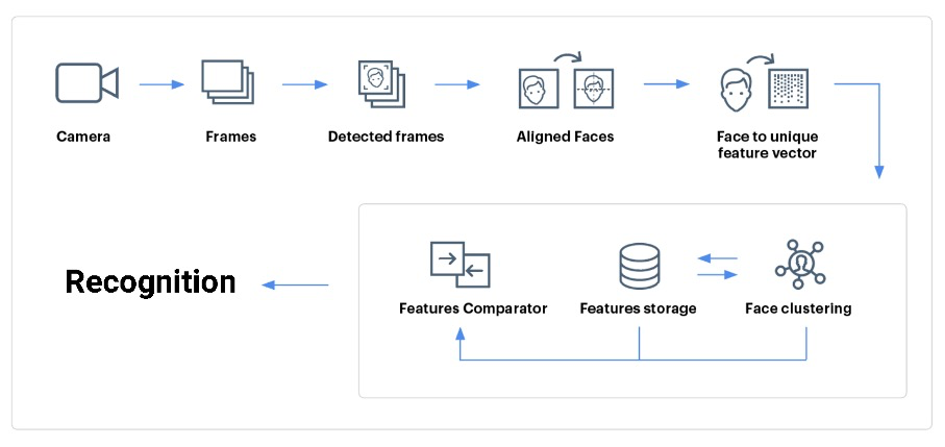
\includegraphics[scale=1]{image1-1}
\caption{ نمای کلی یک سامانه تشخیص چهره \cite{ref20}}
\label{image1-1}
\end{figure}

\section{ الگوریتم‌های استخراج ویژگی و برچسب گذاری تصاویر }
سامانه شناسایی تصویر یکی از مهم ترین بخش‌های یک سامانه بینایی ماشین به حساب می‌آید. این سامانه با استفاده از یادگیری عمیق ، انواع اطلاعات در تصاویر مانند افراد، متون، اشیا و سایر اطلاعات موجود را شناسایی می‌کند. 
الگوریتم‌های مورد استفاده در فرایند تشخیص تصاویر بر مبنای استفاده از ویژگی‌های بصری تصویر مانند لبه و رنگ و یا ویژگی‌های استخراج شده از شبكه‌ عصبی عمیق  به همراه اعمال الگوریتم‌های مختلف خوشه‌بندی ، وایازش  یا طبقه‌بندی  داده‌ها است که سعی در شناسایی و تشخیص تصاویر مختلف دارند. عنصر اصلی این گونه روش‌ها، داده-های مورد استفاده در فرایند یادگیری می‌باشد. نوع و فراوانی داده‌ها در افزایش دقت سامانه‌های تشخیص تصاویر مبتنی بر شبكه‌ عصبی بسیار مهم می‌باشد.


\subsection{ خوشه بندی }
روش خوشه‌بندی بر اساس محاسبه میزان و معیار شباهت در داده‌ها، آن‌ها را در خوشه‌های مختلف قرار می‌دهد. به طور کلی دو نوع روش خوشه‌بندی وجود دارد:

\noindent
خوشه‌بندی سخت : برچسب گذاری به صورت صفر و یک بر روی داده‌ها می‌باشد و مشخص می‌كند داده مورد نظر مربوط به خوشه می‌باشد یا خیر.

\noindent
خوشه‌بندی نرم : به خوشه بندی فازی معروف است و میزان تعلق یک داده به خوشه‌ها را مشخص می‌کند و هر داده می‌تواند با توجه به وزن‌های اختصاص داده شده به آن، به چندین خوشه تعلق داشته باشد.

\noindent
داده‌های استفاده شده در فرایند خوشه بندی، بدون برچسب بوده و یادگیری بدون ناظر  در فرایند خوشه‌بندی داده‌ها استفاده می‌شود. شكل 1-2 نمونه‌ای از خوشه‌بندی سخت و یافتن شاخص برای هر خوشه را نشان می‌دهد.
\begin{figure}[!h]
\centering
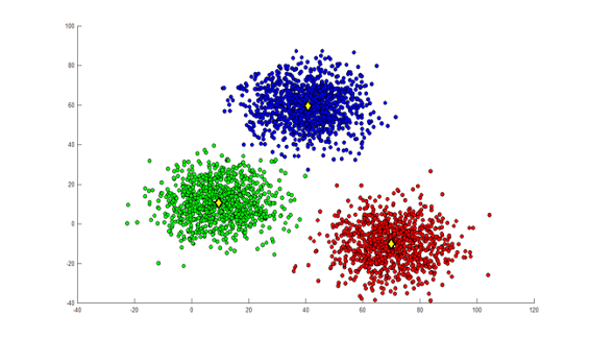
\includegraphics[scale=1]{image1-2}
\caption{ خوشه‌بندی سخت و یافتن شاخص نمونه با توزیع گوسی بر روی داده‌ها \cite{ref20}}\label{image1-2}
\end{figure}

\subsection{طبقه‌بندی}
روش‌های طبقه‌بندی داده‌ها از جمله روش‌های یادگیری با ناظر  هستند که با توجه به یادگیری داده‌های آموزشی به همراه برچسب آن‌ها، داده‌های آزمایشی را نیز برچسب زنی می‌کنند. در طبقه‌بندی داده‌ها می‌توان از توابع سنجش مختلفی برای سنجش میزان تعلق یک داده به هر دسته استفاده کرد. شکل 1-3 یک طبقه‌بند غیر خطی ساده را نشان می‌دهد.

\noindent
در این نوع از الگوریتم‌ها که از لحاظ تعداد، بار اصلی یادگیری ماشین را بر دوش می‌کشند، دو نوع داده وجود دارند. نوع اول داده‌های مستقل نامیده می‌شوند که باید بر اساس آن‌ها، یک متغیر دیگر پیش بینی شود. نوع دوم داده‌های وابسته یا برچسب هستند که قرار است مقادیر آن‌ها به کمک این الگوریتم‌ها پیش بینی شود. برای این منظور باید تابعی ایجاد شود که ورودی‌ها (داده‌های مستقل) را گرفته و خروجی موردنظر (داده‌های وابسته یا هدف) را تولید کنند. فرآیند یافتن این تابع، کشف رابطه‌ای بین متغیرهای مستقل و وابسته است که آن را فرآیند آموزش می‌نامند که بر روی داده‌های موجود اعمال می‌شود و تا رسیدن به دقت لازم ادامه می‌یابد. الگوریتم‌های مختلفی برای طبقه‌بندی داده‌ها وجود دارد که در این میان می‌توان به \lr{SVM} و \lr{KNN} اشاره کرد.

\begin{figure}[h]
\centering
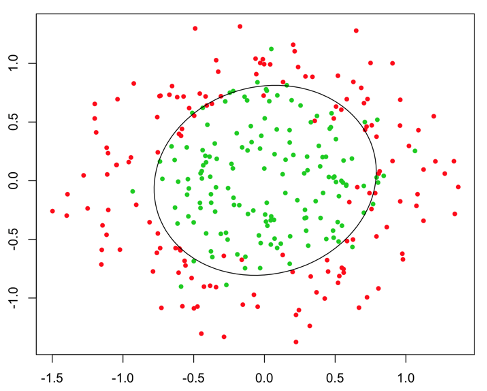
\includegraphics[scale=1]{image1-3}
\caption{ یک طبقه بند غیر خطی ساده \cite{ref19}}\label{image1-3}
\end{figure}

\section{مسئله تشخیص بی‌درنگ چهره در محیط‌های کنترل نشده}
این پایان نامه با محوریت موضوع تشخیص بی‌درنگ چهره افراد در محیط‌های کنترل نشده با در نظر گرفتن شرایط سخت می‌باشد. هدف ما، طراحی و ساخت یک عینک هوشمند مانند شکل 1-4 برای افراد نابینا می‌باشد. هنگامی که شخص نابینا عینک را بر روی چشمانش قرار داده و در محیط‌های عمومی راه می‌رود، دوربینی که بر روی عینک نصب شده است، شروع به بررسی چهره افرادی می کند که در زاویه دید آن قرار دارند. در صورت یافتن یک چهره آشنا، فرد مورد نظر شناسایی شده و نام فرد برای شخص نابینا خوانده می‌شود. این مسئله شامل دو بخش اصلی یافتن چهره و شناسایی چهره می‌شود. هریک از این بخش‌ها و زیر بخش‌های آن‌ها در فصل دوم مورد بررسی قرار خواهند گرفت.

\begin{figure}[!h]
\centering
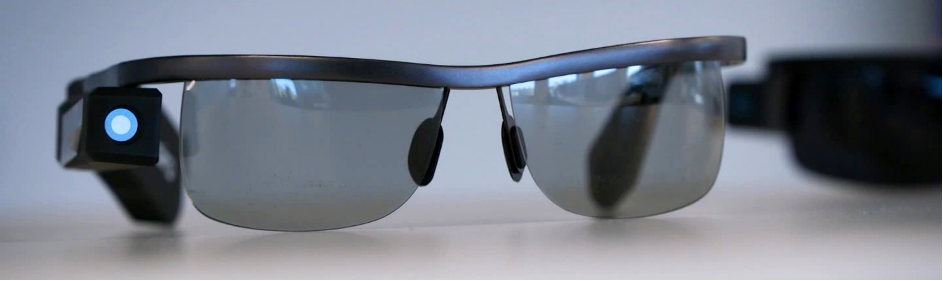
\includegraphics[scale=1]{image1-4}
\caption{نمونه ای از عینک دوربین دار برای افراد نابینا \cite{ref13}}\label{image1-4}
\end{figure}


\subsection{چالش‌های سامانه تشخیص چهره}

سامانه‌های تشخیص چهره به سطح مشخصی از بلوغ رسیده اند، اما توسعه آن‌ها در شرایط کنترل نشده و کاربردهای واقعی هنوز مسیر طولانی در پیش دارد. برای مثال، تشخیص چهره در ویدیویی در محیطی با تغییرات شدید نورپردازی و حالت چهره، انسداد صورت، وضوح پایین تصویر و... ، و ردیابی آن در فریم‌های ویدیو با در نظر گرفتن تناظر بین فریمی و... مشکل می‌باشد. دلیل اصلی به وجود آمدن چالش‌ها این است که چهره انسان یک شی صلب نمی‌باشد و ساختار سه بعدی و پیچیده‌ای دارد و ممکن است تصویر از هر زاویه‌ای گرفته شده باشد. در ادامه مهم ترین چالش‌ها برشمرده شده است.

\noindent
نورپردازی : روشنایی محیط در شب و روز و یا در محیط داخلی و خارجی به شدت تغییر می‌کند. با توجه به ساختار سه بعدی چهره، یک منبع نور مستقیم می‌تواند سایه‌های قوی بر روی چهره ایجاد کند که برخی ویژگی‌های چهره را تغییر می‌دهد. همانطور که در شکل 1-5 نشان داده شده است که گاهی تفاوت‌های ظاهری ناشی از روشنایی، بیشتر از تفاوت بین چهره افراد مختلف می‌باشد.

\begin{figure}[!h]
\centering
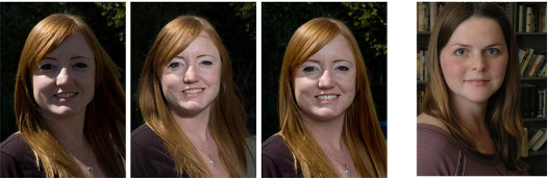
\includegraphics[scale=1]{image1-5}
\caption{مقایسه تفاوت‌های ظاهری ناشی از روشنایی و تفاوت بین چهره افراد \cite{ref13}}\label{image1-5}
\end{figure}

\noindent
حالت : زاویه چهره نسبت به حسگر دوربین، می‌تواند سامانه را با چالش مواجه نماید. چهره با زاویه تند و چهره‌های نیم رخ مانند شکل 1-6 باید برای الگوریتم تشخیص چهره، قابل شناسایی باشند. بنابراین ویژگی‌های استخراج شده توسط الگوریتم باید به گونه‌ای باشند که در هر زاویه‌ای امکان استخراج آن‌ها وجود داشته باشد.
\begin{figure}[!h]
\centering
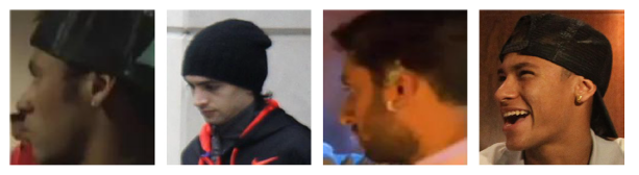
\includegraphics[scale=1]{image1-6}
\caption{زاویه شدید چهره نسبت به دوربین باعث کاهش دقت سامانه می‌شود \cite{ref13}}\label{image1-6}
\end{figure}

\noindent
تاری خارج از تمرکز : اگر عمق میدان دوربین کم باشد و چهره‌ها با فاصله‌های مختلف از دوربین باشند، مشکل تاری خارج از تمرکز رخ خواهد داد (شکل 1-7). اگر دوربین طوری تنظیم شود که چهره نزدیک‌تر، واضح‌تر دیده شود، در مقابل باعث می‌شود که چهره دورتر، مقداری مات شود و برعکس. این مسئله می‌تواند برای سامانه تشخیص چهره دردسر ساز شود.
\begin{figure}[!h]
\centering
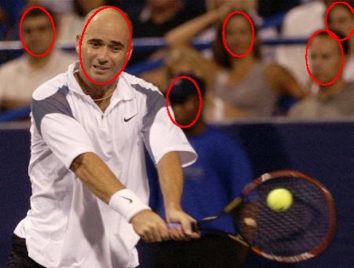
\includegraphics[scale=1]{image1-7}
\caption{تاری خارج از تمرکز به علت عمق کم میدان دوربین \cite{ref13}}\label{image1-7}
\end{figure}

\noindent
انسداد : اگر در حال تصویر برداری از یک جمع باشیم، احتمال اینکه چهره فردی توسط فرد دیگری مقداری پوشانده شود، بسیار بالاست. همچنین اگر موهای فرد بر روی صورتش ریخته باشد، از عینک آفتابی استفاده کند، یا نورپردازی غیر یکنواخت باشد (شکل 1-8)، انسداد چهره رخ خواهد داد.
\begin{figure}[!h]
\centering
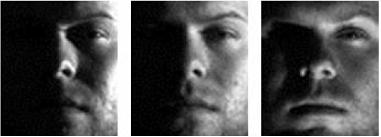
\includegraphics[scale=1]{image1-8}
\caption{انسداد شدید در اثر نورپردازی \cite{ref13}}\label{image1-8}
\end{figure}

\noindent
سن : بیشتر روش‌های مرسوم تشخیص چهره تغییرات سن را نادیده می‌گیرند. بعضی از رویکردها به طور منظم پایگاه داده تصاویر را به روز رسانی کرده و بازآموزی سامانه را انجام می‌دهند. این راه حل فقط برای سامانه‌هایی مناسب است که اغلب وظیفه احراز هویت کارمندان را انجام می‌دهد. در شرایط دیگر سن موضوع را باید جدی گرفت و تلاش کرد تا سامانه نسبت به این نوع تغییرات قوی‌تر شود.

\noindent
کمبود داده‌های آموزشی: سامانه‌های تشخیص چهره در کاربردهای واقعی دارای مشکل کمبود داده‌های آموزشی برای آموزش سامانه می‌باشند. تعداد افراد در محیط کنترل نشده زیاد می‌باشد و به قادر به در اختیار داشتن حجم بالایی از داده‌های آموزشی برای هر کدام از افراد نیستیم. از طرفی کاهش تعداد داده‌های آموزشی می‌تواند دقت سامانه را به شدت کاهش دهد. 

\noindent
منابع محدود: در صورت اجرای پردازش‌های سامانه توسط تلفن همراه، باید محدودیت منابع را در نظر گرفت. تلفن همراه نسبت به رایانه، دارای قدرت پردازنده پایین‌تر و منبع انرژی محدودتر می‌باشد که باعث می‌شود الگوریتم‌هایی با پیچیدگی محاسباتی بالا بر روی این دستگاه‌ها قابل اجرا نباشد. بنابراین الگوریتم استفاده شده باید دارای کمترین پیچیدگی زمانی و حافظه باشد.

\noindent
زمان: یکی از چالش‌های موجود، فضایی پر از چهره‌های مختلف در مکان‌های عمومی و در مقابل، نیاز به واکنش سریع توسط سامانه است. مشابه شکل 1-9 در فضاهای عمومی و معابر پیاده مردم با سرعت از کنار دوربین عبور می-کنند و سامانه باید قابلیت تشخیص چهره آن‌ها در چند ثانیه را داشته باشد. اگر کاربر سامانه با افراد جدید دیدار داشته باشد، سامانه باید به سرعت یاد بگیرد که چهره افراد جدید را تشخیص دهد. 

\begin{figure}[!h]
\centering
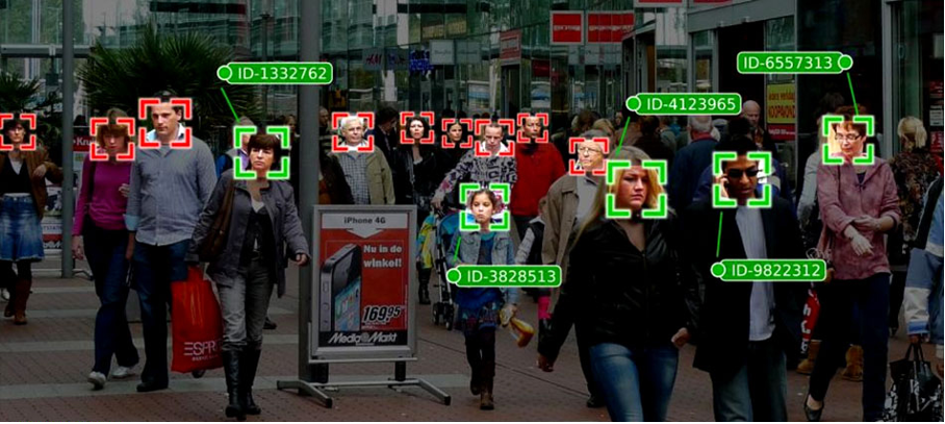
\includegraphics[scale=1]{image1-9}
\caption{نمونه ای از یک سامانه تشخیص چهره بی‌درنگ در محیط کنترل نشده \cite{ref13}}\label{image1-9}
\end{figure}
 
%\chapter{ مروری بر کارهای گذشته}

\section{مقدمه}
همانطور که در فصل مقدمه بیان شد، دو موضوع یافتن چهره \LTRfootnote{Face Detection} در تصویر و شناسایی چهره \LTRfootnote{Face Recognition}، بخش‌های اصلی سامانه تشخیص چهره می‌باشند. اگرچه این دو بخش برای انسان کار ساده ای به نظر می‌رسد، اما برای کامپیوتر‌ها همیشه با چالش همراه بوده است. دلیل این سختی می‌تواند تفاوت تصویرها در مقیاس، حالت چهره، پس زمینه، تابش نور، انسداد و... باشد. در ادامه به بررسی روش‌هایی برای یافتن و شناسایی چهره در دو بخش مجزا پرداخته شده است.
\section{یافتن چهره}
یافتن مکان چهره در تصویر، اولین گام در فرایند تشخیص چهره می‌باشد که نقشی کلیدی در سامانه ایفا می‌نماید. هدف اصلی الگوریتم‌ یافتن چهره این است که تعیین کند آیا چهره ای در تصویر وجود دارد یا خیر و در صورت وجود چهره، مکان آن را بیابد. یافتن چهره در تصویر، امری پیچیده است. زیرا چهره انسان همواره دستخوش تغییراتی مانند شرایط روشنایی و وضوح تصویر، حالت چهره، رنگ پوست، حضور عینک یا موی صورت و... می‌شود. در سال 2002 \lr{Yang} و همکاران در \cite{982883} یک دسته بندی برای روش‌های یافتن چهره ارائه کردند که در ادامه شرح داده می‌شود.

\subsection{رویکردهای مبتنی بر دانش}
این رویکردها به مجموعه‌ای از قوانین بستگی دارند و بر اساس دانش انسان در مکان قرار گرفتن اجزای چهره و ویژگی-های خاصی که در چهره انسان وجود دارد، عمل می‌کنند. یافتن یک جفت چشم در تصویر و سپس جستجو اطراف آن برای یافتن چهره، مثالی از این روش می‌باشد. ابتدا مکان چشم‌ها و بالاترین نقطه سر پیدا می‌شود. سپس فاصله بین چشم تا بالاترین نقطه محاسبه شده و به عنوان یک مرجع برای یافتن نواحی دیگر مانند بینی و دهان مورد استفاده قرار می‌گیرد. این روش زمانی که مو بر روی پیشانی ریخته باشد یا در حضور عینک، به درستی عمل نمی‌کند. یا به عنوان مثال:


\begin{itemize}
\item
 هر چهره داری دو فرو رفتگی برای چشم ها است و چیزی شبیه به ابرو روی این فرو رفتگی‌ها قرار دارد.
 \item
صورت شامل بینی، چشم‌ها و دهان در فاصله‌ها و موقعیت‌های خاصی با یکدیگر می‌باشد.
 \item
چهره مانند یک ناحیه کوچکتر است که بر روی یک ناحیه بزرگتر مانند شانه‌ها قرار گرفته است. 
 \item
چهره انسان متقارن است.

\end{itemize} 
	
مشکل بزرگ این رویکرد‌ها، ساختن یک مجموعه مناسب از قوانین است. اگر قوانین خیلی ساده یا خیلی دقیق باشند، الگوریتم همیشه به درستی عمل نمی‌کند. این رویکرد به تنهایی کافی نیست و موفق به یافتن چهره‌ها در شرایط کنترل نشده با تعداد زیادی چهره نمی‌باشد.

\subsection{رویکردهای مبتنی بر تطبیق کلیشه یا الگو}
این رویکرد با استفاده از قالب \LTRfootnote{Template} ‌های از پیش تعیین شده برای یافتن چهره‌ها با همبستگی بین الگوها و تصاویر ورودی استفاده می‌نماید. چهره انسان را می‌توان به چشم، صورت، بینی و دهان تقسیم کرد. همچنین، با استفاده از روش تشخیص لبه، یک مدل صورت می‌تواند توسط لبه‌ها ساخته شود. شکل 2-1 یک نمای کلی از رویکرد مبتنی بر کلیشه را نشان می‌دهد. این رویکرد ساده است، اما برای تشخیص چهره ناکافی است. با این حال، قالب‌های انعطاف پذیر برای مقابله با این مشکلات پیشنهاد شده اند.


\begin{figure}[h]
\centering
  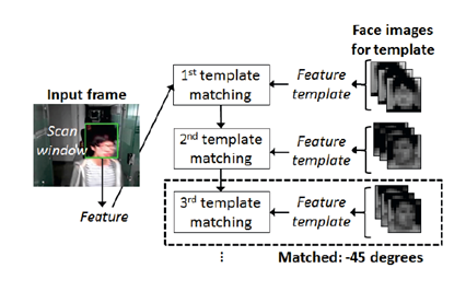
\includegraphics[scale=1]{image2-1}
  \caption{رویکرد مبتنی بر تطبیق کلیشه  \cite{ref1}.}
  \label{image2-1}
\end{figure}

\subsection{رویکردهای مبتنی بر ویژگی}
این رویکردها‌ با استخراج ویژگی \LTRfootnote{Feature} ‌های ساختاری چهره، چهره‌ها را پیدا می‌نمایند. ابتدا به عنوان یک طبقه‌بند، آموزش دیده و سپس برای تمایز میان نواحی شامل چهره و بدون چهره در تصویر استفاده می‌شوند. ایده این رویکرد، غلبه بر محدودیت دانش ما از چهره‌ها می‌باشد. در \cite{HJELMAS2001236} تعدادی از این رویکردها مورد بررسی قرار گرفته است:

\subsubsection{رویکرد مبتنی بر حرکت}
اگر یک توالی از چند فریم در اختیار باشد، می‌توان به کمک اطلاعات حرکت \LTRfootnote{Motion}، یافتن چهره را انجام داد. برای این کار به کمک تفاصل فریم‌ها، قسمت متحرک نسبت به پس زمینه شناسایی شده و بخش بالای آن جدا می‌شود. بدین ترتیب می‌توان با احتمال بالا، مکان چهره یک فرد را در یک تصویر پیدا نمود. این رویکرد در مواجه با اجسام متحرک دیگری مانند اتومبیل دچار اشتباه می‌شود.

\subsubsection{رویکرد مبتنی بر لبه}
ابتدا به کمک یک الگوریتم لبه یاب \LTRfootnote{Edge Detection}، لبه‌های تصویر بدست می‌آید، سپس نازک سازی می‌شوند و شاخه‌های اضافه حذف می‌گردد (شکل 2-2). گوشه لبه‌ها تشخیص داده می‌شوند و هر مولفه متصل \LTRfootnote{Connected Component} به شاخه مرکزی آن کاهش می‌یابد. اجزایی که ویژگی چهره در آن‌ها نیست حذف می‌شوند و اجزای نهایی به عنوان سمت چپ چهره، خط مو، یا سمت راست چهره برچسب گذاری می‌شوند. در یک آزمایش که 60 تصویر دارای پس زمینه پیچیده حاوی 90 چهره به این سامانه داده شده است، سامانه قادر به یافتن 76\% چهره‌ها بوده است.

\begin{figure}[h]
\centering
  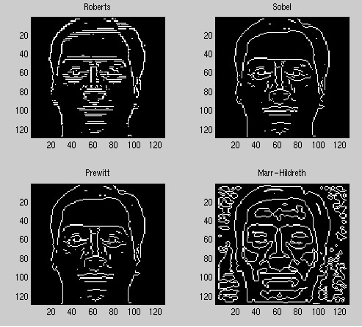
\includegraphics[scale=0.6]{image2-2}
  \caption{استفاده از لبه یاب های معروف برای استخراج ویژگی های مبتنی بر لبه از چهره  \cite{ref1}.}
  \label{image2-2}
\end{figure}

\subsubsection{رویکرد مبتنی بر اطلاعات سطح خاکستری} 
سطوح خاکستری \LTRfootnote{Gray level} تصویر چهره شامل اطلاعات مفیدی می‌باشد. برای مثال ابرو‌ها، مردمک چشم و لب‌ها معمولا تاریک تر از سایر نواحی صورت هستند. این ویژگی‌ها می‌تواند به یافتن یک چهره در تصویر کمک نماید. در این رویکرد ابتدا بر روی تصویر ورودی، عملیات بسط تباین \LTRfootnote{Contrast Stretching} و عملیات مورفولوژی \LTRfootnote{Morphological Oparations} مبتنی بر سطح خاکستری انجام می‌شود تا تصویر بهبود پیدا کند و یافتن نواحی تیره تر، راحت شود. سپس تصویر به چندین بخش تقسیم می‌شود و سطوح خاکستری بخش‌ها مورد بررسی قرار می‌گیرد. مزیت این رویکرد، کارایی در تصاویر با وضوح پایین می‌باشد (شکل 2-3).

\begin{figure}[h]
\centering
  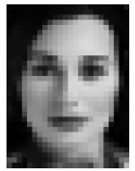
\includegraphics[scale=0.6]{image2-3}
  \caption{اطلاعات سطح خاکستری حتی در وضوح پایین نیز قابل دسترسی می باشند  \cite{ref1}.}
  \label{image2-3}
\end{figure}

\subsubsection{رویکرد مبتنی بر اطلاعات رنگی}
رنگ در تصویر اطلاعات با ارزشی به ما می‌دهد و می‌توان از رنگ پوست انسان برای یافتن چهره در تصویر استفاده کرد. برای این کار ابتدا رنگ‌ها هنجار سازی \LTRfootnote{Normalization} می‌شوند تا اثر نور پردازی از بین برود. گسترده ترین فضای رنگ مورد استفاده RGB می‌باشد.
\begin{equation}\label{eq2-1}
r = \frac{R}{R + G + B}
\end{equation}

\begin{equation}\label{eq2-2}
g = \frac{G}{R + G + B}
\end{equation}

\begin{equation}\label{eq2-3}
b = \frac{B}{R + G + B}
\end{equation}

در روابط بالا \lr{R} میزان سطح رنگ قرمز، \lr{G} میزان سطح رنگ سبز و \lr{B} میزان سطح رنگ آبی در هر پیکسل از تصویر می‌باشد. 
\lr{r}
، 
\lr{g}
و
\lr{b}
به ترتیب مقدار هنجار سازی شده برای رنگ قرمز، سبز و آبی می‌باشد. واضح است که:
    
\begin{equation}\label{eq2-3}
r + g + b = 1
\end{equation}
 	
پس می‌توان فقط با داشتن مقدار \lr{r} و \lr{g} مقدار \lr{b} را بدست آورد. با توجه به بافت‌نگار \LTRfootnote{Histogram} رنگ سبز و قرمز تصویر، رنگ پوست انسان، بخش کوچکی از بافت‌نگار را اشغال می‌کند. بنابراین با بررسی پیکسل‌های تصویر، می‌توان با دقت بالایی احتمال حضور چهره در تصویر را تشخیص داد و رنگ پوست انسان را می‌توان به راحتی با یک تابع گوسی تخمین زد. فضاهای رنگی دیگری نیز در این زمینه مورد استفاده قرار گرفته است. مانند
\lr{HSV},
\lr{YIQ},
\lr{YES},
\lr{YCrCb},
\lr{Lab}.
یک ایده خوب این است که وقتی شخص از دوربین فاصله زیادی دارد از رنگ پوست استفاده کنیم و وقتی شخص نزدیک به دوربین می‌باشد از ویژگی‌های قدرتمندتر چهره استفاده نماییم.

\subsection{رویکرد مبتنی بر عامل‌های آماری}
رویکرد‌های بخش‌های قبل بر روی اطلاعات استخراج شده از تصاویر چهره در شرایط آزمایشگاهی تکیه می‌کنند و اگر یک تصویر چهره در شرایط کنترل نشده و پس زمینه پیچیده داده شود، بسیاری از این رویکردها شکست می‌خورند. استفاده از عامل‌های آماری \LTRfootnote{Statistical Parameters} برای ویژگی‌ها و ارائه یک مدل احتمالی برای چهره، باعث انعطاف پذیری بیشتر سامانه می-شود. این رویکرد قادر است در مواجه با جا به جایی، چرخش و تغییر مقیاس با دقت بیشتری عمل نماید. در یک رویکرد دقیق‌تر از شبکه‌های بیز \LTRfootnote{Bayes Rule} برای یافتن احتمالاتی چهره بهره گرفته شده است. یافتن چهره در حضور عینک و برخی ویژگی‌های از دست رفته نیز توسط این رویکرد انجام می‌شود.

\noindent
تا به امروز صدها رویکرد برای یافتن چهره ارائه شده است تا آن را پیشرفته تر و دقیق تر نماید، اما انقلاب الگوریتم‌های یافتن چهره در سال 2001 بود. زمانی که \lr{Viola} و \lr{Jones} در \cite{990517} یک الگوریتم چهره یاب بی‌درنگ معرفی کردند که قادر به یافتن چهره با دقت بالا بود. در ادامه به شرح این الگوریتم می‌پردازیم.

\noindent
پیش پردازش: ابتدا تصویر از فضای \lr{RGB} به تصویر سطح خاکستری تبدیل می‌شود. زیرا تشخیص چهره‌ها در تصویر خاکستری برای سامانه آسان است. سپس در صورت نیاز، پیش پردازش‌هایی مانند تغییر اندازه \LTRfootnote{Resizing}، برش \LTRfootnote{Cropping}، تار شدن \LTRfootnote{Blurring} و تیزکردن لبه های تصویر \LTRfootnote{Sharpening} انجام می‌شود. 

\noindent
ویژگی‌های \lr{Haar}: تمام چهره‌های انسانی ویژگی‌های مشترکی دارند. برای مثال ناحیه چشم تاریک‌تر از پیکسل‌های همسایه آن است و ناحیه بینی از چشم روشن‌تر است. ویژگی‌های \lr{Haar} مستطیل‌هایی هستند که نشان دهنده بخش‌های مختلف صورت می‌باشند. شکل ‏2-4 نمونه‌هایی از مستطیل‌های ویژگی‌های \lr{Haar} را نشان می‌دهد.
\begin{figure}[h]
\centering
  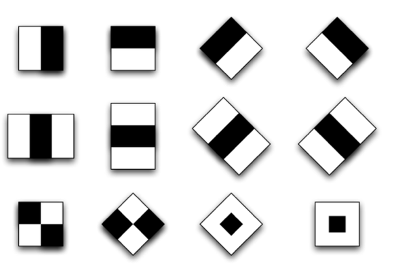
\includegraphics[scale=1]{image2-4}
  \caption{نمونه هایی از مستطیل های ویژگی های Haar \cite{ref1}.}
  \label{image2-4}
\end{figure}

\noindent
ویژگی‌های‌ \lr{Haar} برای تشخیص چشم، بینی، دهان و... با کمک تشخیص لبه، تشخیص خط و تشخیص مرکز در تصویر و استخراج ویژگی برای یافتن چهره استفاده می‌شود. مستطیل‌های ویژگی‌های \lr{Haar}، متناسب با بخش‌های چهره می‌باشند که مثالی از آن در شکل 2-5 نشان داده شده است.

\begin{figure}
\begin{subfigure}{.5\textwidth}
  \centering
  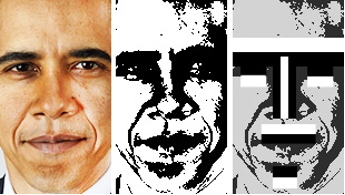
\includegraphics[scale=1]{image2-5-a}
  \label{image2-5-a}
\end{subfigure}
\begin{subfigure}{.5\textwidth}
  \centering
  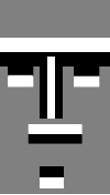
\includegraphics[scale=1]{image2-5-b}
  \label{image2-5-b}
\end{subfigure}
\caption{مستطیل های ویژگی های Haar متناسب با بخش های چهره می باشند \cite{ref1}.}
\label{fig:image2-5}
\end{figure}

\noindent
همانطور که در شکل 2-6 مشاهده می‌شود، هر مستطیل در بخش‌های مختلف چهره در روندی تکراری با اندازه‌های مختلف قرار می‌گیرد و نتیجه نهایی از کم کردن مجموع سطح روشنایی پیکسل‌های زیر بخش‌های سیاه از مجموع سطح روشنایی پیکسل‌های زیر بخش‌های سفید به دست می‌آید که یک عدد می‌باشد. از یک پنجره با اندازه ۲۴×۲۴ برای قرار دادن مستطیل‌ها بر روی تصویر استفاده می‌شود که تعداد زیاد و اندازه‌های مختلف آن‌ها باعث می‌شود برای محاسبه نتیجه نهایی نیاز به انجام بیش از ۱۶۰۰۰۰ محاسبه باشد که زمان زیادی برای هر تصویر خواهد گرفت.

\begin{figure}[h]
\centering
  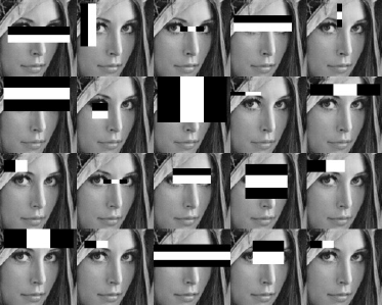
\includegraphics[scale=1]{image2-6}
  \caption{هر مستطیل در اندازه های مختلف بر روی بخش های مختلف تصویر قرار می گیرد \cite{ref1}.}
  \label{image2-6}
\end{figure}

\noindent
\lr{Ada Boost}: 
همانطور که در شکل 2-7 مشاهده می‌شود، تمام ویژگی‌های Haar برای تصویر ورودی مناسب نخواهد بود. بعضی از این ویژگی‌ها باید نادیده گرفته شوند و فقط ویژگی‌های مرتبط انتخاب شوند تا در زمان صرفه جویی شود. این کار به صورت خودکار به کمک عنصر Ada Boost انجام می‌شود.
\begin{figure}[h]
\centering
  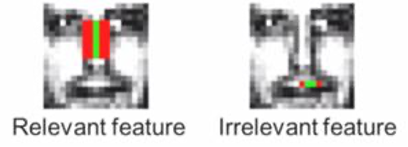
\includegraphics[scale=1]{image2-7}
  \caption{یک ویژگی مرتبط در مقابل یک ویژگی نامرتبط \cite{ref1}.}
  \label{image2-7}
\end{figure}

\noindent
\lr{Ada Boost} 
یک الگوریتم مبتنی بر یادگیری ماشین می‌باشد که ویژگی‌های کاربردی را از میان تعداد زیادی ویژگی پیدا می‌کند. بعد از شناسایی ویژگی‌های مختلف، مشخص می‌گردد که هر یک از پنجره‌ها برای بخشی از چهره مناسب می‌باشد یا خیر. هر کدام از ضرایب انتخاب شده مثبت در نظر گرفته می‌شود، در صورتی که حداقل بتواند بیش از نیمی از موارد را تشخیص دهد. این ویژگی‌ها با عنوان طبقه‌بندهای ضعیف
 \LTRfootnote{Weak Classifier} 
 معرفی می‌شوند. 
\lr{Ada Boost} 
در طبقه‌بند قوی \LTRfootnote{Strong Classifier}، تعداد زيادی طبقه‌بند ضعيف را با هم ترکيب مي‌کند. رابطه کلی آن به صورت زیر می‌باشد.
\begin{equation}\label{eq2-5}
F(x)=α_1 f_1 (x)+α_2 f_2 (x)+⋯
\end{equation}

\noindent
که در آن \lr{F} طبقه‌بند قوی می‌باشد که از تعدادی f\textsubscript{i} که طبقه‌بند ضعیف می‌باشد، تشکیل شده است. هر کدام از طبقه‌بندهای ضعیف، یک خروجی صفر یا یک تولید می‌کنند. α\textsubscript{i} وزن مربوط به طبقه‌بند می‌باشد. با استفاده از این الگوریتم و وزن دادن به ویژگی‌ها، بیش از ۱۶۰۰۰۰ ویژگی قبلی به کمتر از ۲۵۰۰ ویژگی کاهش پیدا می‌کند.

\noindent
تصویر یکپارچه \LTRfootnote{Integral Image}: تصویر یکپارچه، یا جدول محدوده مجتمع \LTRfootnote{Summed area table}، به منظور ارزيابی سريع‌تر ویژگی‌هایی که در بخش اول معرفی شد، استفاده می‌شود. با توجه به شکل 2-8 در یک تصویر یکپارچه مقدار پیکسل در مکان \lr{x} و \lr{y} برابر با جمع مقادیر پیکسل‌های بالا و چپ پیکسل \lr{x} و \lr{y} می‌باشد.

\begin{figure}[h]
\centering
  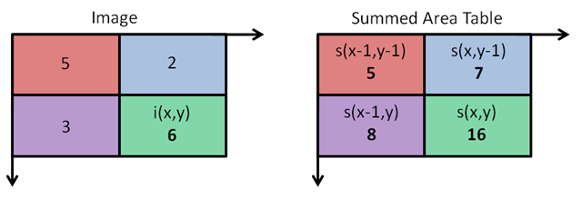
\includegraphics[scale=1]{image2-8}
  \caption{نحوه مقدار دهی به پیکسل های تصویر یکپارچه \cite{ref1}.}
  \label{image2-8}
\end{figure}

\noindent
به عنوان مثال در شکل 2-9 مقدار پیکسل‌ها به صورت زیر محاسبه می‌شود:
\begin{itemize}
\item
مقدار پیکسل ۱ در تصویر یکپارچه برابر است با مجموع پیکسل‌ها در مستطیل \lr{A}.
 \item
مقدار پیکسل ۲ در تصویر یکپارچه برابر است با مجموع پیکسل‌ها در مستطیل \lr{A} و \lr{B}.
 \item
مقدار پیکسل ۳ در تصویر یکپارچه برابر است با مجموع پیکسل‌ها در مستطیل \lr{A} و \lr{C}.
 \item
مقدار پیکسل ۴ در تصویر یکپارچه برابر است با مجموع پیکسل‌ها در مستطیل \lr{A} و \lr{B} و \lr{C} و \lr{D}.
\item
مجموع پیکسل‌ها در مستطیل \lr{D} می‌تواند به صورت (۳+۲) - (۱+۴) محاسبه شود.

\end{itemize} 


\begin{figure}[h]
\centering
  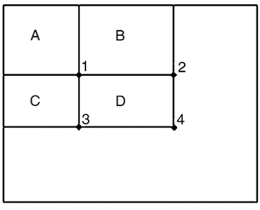
\includegraphics[scale=1]{image2-9}
  \caption{بخشی از یک تصویر که تصویر یکپارچه آن محاسبه می شود \cite{ref1}.}
  \label{image2-9}
\end{figure}

\noindent
مراحل آبشاری \LTRfootnote{Cascading}: اگر تصویر به مربع‌های ۲۴×۲۴ پیکسلی تقسیم شده و با پردازش هر بخش که ۲۵۰۰ ویژگی دارد، تشخیص داده شود که چهره‌ای در تصویر وجود دارد یا خیر، حجم محاسبات بسیار زیاد خواهد بود. مراحل آبشاری این فرایند را سریع‌تر انجام می‌دهد. ۲۵۰۰ ویژگی هر مربع ۲۴×۲۴ به دسته‌بندی‌های مختلف تقسیم می‌شود. برای مثال ۱۰ ویژگی در دسته‌ اول، ۲۰ ویژگی در دسته دوم، ۱۰۰ ویژگی در دسته سوم و... . می‌توان بعد از پردازش هر دسته، در ارتباط با وجود یا عدم وجود چهره در آن دسته تصمیم گرفت تا بخش‌هایی که چهره در آن وجود ندارد زودتر حذف شوند. شکل 2-10 یک نمای کلی از روند تشخیص آبشاری را نشان می‌دهد. مجموعه ای از طبقه‌بندها به هر زیر پنجره اعمال می‌شود. طبقه بند اولیه تعداد زیادی از نمونه‌های منفی را حذف می‌کند و پردازش کمی دارد. لایه‌های بعد، منفی‌های اضافی را حذف می‌کنند که نیاز به محاسبات بیشتری دارند. این الگوریتم عملکرد بسیار خوبی در برنامه‌های کاربردی بی‌درنگ و در حضور پس زمینه‌های شلوغ نشان داده است. اما هنوز در برای چهره‌هایی که رو به روی دوربین نیستند، تغییرات شدید نور، انسداد و... دارای چالش می‌باشد.

\begin{figure}[h]
\centering
  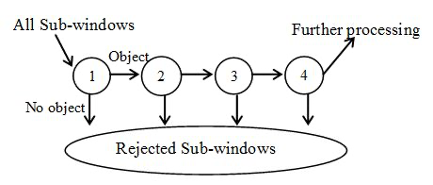
\includegraphics[scale=1]{image2-10}
  \caption{بخشی از یک تصویر که تصویر یکپارچه آن محاسبه می شود \cite{ref1}.}
  \label{image2-10}
\end{figure}

\noindent
در سال ۲۰۰۵ \lr{Dalal} و همکاران در \cite{1467360} روشی به نام بافت نگار شیب‌های جهت دار \LTRfootnote{Histograms Of Oriented Gradients} ارائه کردند که به اختصار \lr{HOG} نامیده می‌شود. در این روش ابتدا تصویر خاکستری می‌شود، زیرا نیازی به رنگ نیست. پیرامون هر پیکسل بررسی می‌شود تا مشخص شود نسبت به پیکسل‌های پیرامونش چقدر تاریک می‌باشد. مطابق شکل 2-11 جهتی انتخاب می‌شود که به سمت پیکسل‌های تاریکتر باشد. این روند برای همه پیکسل‌های تصوير انجام می‌شود و به ازای هر پیکسل یک جهت ذخیره خواهد شد که روندی از روشنايى به تاريكى را در تصوير نمايش مي‌دهند.

\begin{figure}
\begin{subfigure}{.5\textwidth}
  \centering
  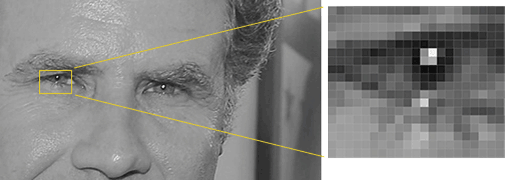
\includegraphics[width=1.0\textwidth]{image2-11-a}
  \label{image2-11-a}
\end{subfigure}
\begin{subfigure}{.5\textwidth}
  \centering
  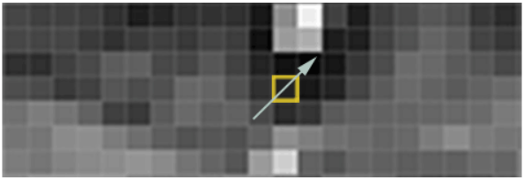
\includegraphics[width=1.0\textwidth]{image2-11-b}
  \label{image2-11-b}
\end{subfigure}
 \caption{سطح روشنایی پیکسل های اطراف هر پیکسل بررسی شده و راستای روشن به سمت تاریک برگزیده می شود \cite{ref1}.}
\label{fig:image2-11}
\end{figure}

\noindent
دليل استفاده از جهت‌ها این است که اگر پیکسل‌ها به طور مستقيم استفاده شوند، تصوير تاريك و تصوير روشن از يك چهره مشخص، دارای سطح روشنایی متفاوتى خواهند بود. اما با در نظر گرفتن جهتى تغییر روشنايى، هم تصوير تيره و هم تصوير روشن، نمايش يكسانى خواهند داشت كه حل مسئله را آسان‌تر مي‌كند.
ذخيره جهت‌ها براى تمام پیکسل‌ها باعث افزایش جزئيات می‌شود. لذا روند اصلى روشنايى و تاريكى در سطحی بالاتر در نظر گرفته می‌شود، به طورى كه بتوان الگوى اصلى تصوير را ديد. تصوير به بخش‌هاى ١٦×١٦ پيكسل تقسیم می-شود و در هر بخش تعداد جهت‌هاى به سمت بالا، پايين، چپ و راست شمارش مي‌شود. سپس بخش‌هاى درون تصوير با جهت‌هايى كه بزرگتر بودند، جايگزين مي‌شود. نتيجه نهايى، تبديل تصوير به يك نمايش ساده شده از ساختار چهره است که در شکل 2-12 مشاهده می‌شود. براى يافتن چهره‌ها در این الگوریتم، بخش‌هايى از تصوير كه به الگوى \lr{HOG} شبيه‌تر است، مشخص می‌شود. با استفاده از اين روش، مي‌توان چهره‌ها را در تصویر به سادگى پيدا كرد.

\begin{figure}
\begin{subfigure}{.5\textwidth}
  \centering
  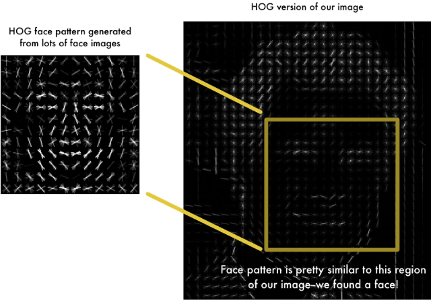
\includegraphics[scale=1]{image2-12-a}
  \label{image2-12-a}
\end{subfigure}
\begin{subfigure}{.5\textwidth}
  \centering
  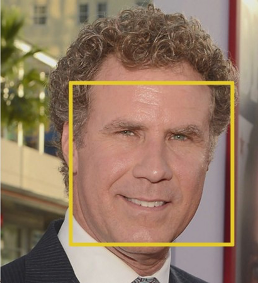
\includegraphics[scale=1]{image2-12-b}
  \label{image2-12-b}
\end{subfigure}
  \caption{براى يافتن چهره ها، بخش هايى از تصوير كه به الگوى HOG شبيه تر است را پيدا می كنيم \cite{ref1}.}
\label{fig:image2-12}
\end{figure}

در سال 2015 \lr{Shengcai Liao} و همکاران در \cite{7130626} یک روش دقیق و سریع برای یافتن چهره ارائه دادند که در آن از اختلاف پیکسل هنجارسازی شده یا \lr{NDP} برای یافتن چهره استفاده می‌شود. ارزیابی ویژگی \lr{NPD} بسیار سریع است و دسترسی به حافظه تنها با استفاده از یک جدول جستجو می‌باشد. در این روش نشانه گذاری یا خوشه بندی در مرحله آموزش نیز لازم نیست و در برابر تغییرات نور، حالت، انسداد، تصاویر با وضوح پایین و... مقاوم است. \lr{NPD} بین دو پیکسل در یک تصویر به صورت زیر تعریف شده است:
\begin{equation}\label{eq2-6}
f(x,y) = \frac{x - y}{x + y}
\end{equation}

\noindent
که در آن \lr{x} و \lr{y} بزرگتر از صفر هستند و \lr{f(0,0)} برای حالتی که \lr{x = y = 0} باشد، برابر صفر است. این عمل بر روی هر جفت پیکسل از تصویر اجرا می‌شود. اگر تصویر ورودی مربعی با ابعاد \lr{s} باشد و \lr{p=s×s} تعداد پیکسل‌ها باشد، آنگاه تعداد ویژگی‌های استخراج شده برابر \lr{d=p(p-1)/2} می‌باشد. سپس علامت \LTRfootnote{Sign} ویژگی‌های استخراج شده مورد استفاده قرار می‌گیرد که وابسته به اندازه سطح روشنایی پیکسل‌ها نمی‌باشد. بلکه تنها نشان می‌دهد کدام ناحیه روشن‌تر و کدام ناحیه تیره‌تر می‌باشد. همچنین این ویژگی‌ها به خدشه \LTRfootnote{Noise} حساس نمی‌باشند. در نهایت ویژگی‌های استخراج شده به عنوان ورودی به یک سامانه یادگیری داده می‌شود. نمونه‌ای از نتیجه اجرای این الگوریتم بر روی مجموعه داده \lr{FDDB} در شکل 2-13 آمده است.
 
 \begin{figure}[h]
\centering
  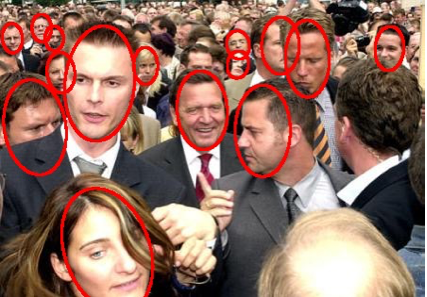
\includegraphics[scale=1]{image2-13}
  \caption{نتیجه اجرای روش مبتنی بر NPD \cite{ref1}.}
  \label{image2-13}
\end{figure}

\noindent
تمام رویکرد‌های ارائه شده که یافتن چهره را با مدل سازی صریح از ویژگی‌های صورت انجام می‌دهند، در برابر تغییرات غیر قابل پیش بینی چهره و شرایط محیطی دچار مشکل می‌شوند. اگرچه بعضی از تلاش‌های اخیر مبتنی بر ویژگی، توانایی مقابله با شرایط کنترل نشده را بهبود داده اند، اما بیشتر آن‌ها هنوز به چهره‌های رو به رو و شرایط کنترل شده محدود می‌شوند، و به عنوان یکی از روش‌های یک سامانه ترکیبی در نظر گرفته شده اند. پس نیاز به روش-هایی هست که بتوانند در شرایط خصمانه تر مانند تشخیص چهره‌های متعدد در زمینه‌های شلوغ به خوبی عمل کنند.

 \subsection{رویکردهای مبتنی بر تصویر}
رویکردهای مبتنی بر تصویر نیاز به مجموعه‌ای از تصاویر آموزشی برای پیدا کردن مدل‌های چهره دارند و بر اساس استخراج ویژگی و یادگیری ماشین عمل می‌نمایند. مجموعه‌ای از تصویر‌های مختلف چهره طبقه‌بندی می‌شوند و برای تشخیص چهره جدید از این طبقه‌بندی استفاده می‌شود. نمونه‌هایی از چهره و نمونه‌هایی از غیر چهره به طبقه‌بند داده می-شود تا از روی این تصویرها عمل یادگیری انجام شود. به طور تجربی دقت نتایج رویکردهای مبتنی بر تصویر بهتر از سایر رویکرد‌ها می‌باشد. این رویکردها به چند دسته تقسیم می‌شوند که در ادامه شرح داده شده است. 

 \subsubsection{رویکرد مبتنی بر ماشین بردار پشتیبان}
ماشین‌ بردار پشتیبان  طبقه‌بندی خطی می‌باشد که حاشیه بین ابرصفحه تصمیم و داده‌های آموزش را به حداکثر می-رساند. برای اولین بار در سال 1997 \lr{Osuna} و همکاران در \cite{609310} از این طبقه‌بند برای یافتن چهره استفاده کردند.

 \subsubsection{رویکرد مبتنی بر شبکه‌ عصبی}
یک راه حل غیر خطی برای یافتن چهره، استفاده از شبکه‌های عصبی \LTRfootnote{Neural Network} است. اولین رویکردهای عصبی در یافتن چهره بر اساس \lr{MLP} بود که در مجموعه داده‌های ساده، امیدوار کننده بود. شبکه‌های عصبی با معماری پیمانه ای \LTRfootnote{Modular Architecture} امروزی بسیار پیچیده‌تر از \lr{MLP} \LTRfootnote{Multi Layer Perceptron} ساده هستند. نوع خاصی از شبکه‌های عصبی عمیق برای پردازش تصاویر استفاده می‌شوند که شبکه عصبی پیچشی \LTRfootnote{Convolutional Neural Network}  نام دارند. ساختار عمیق این شبکه‌ها باعث شد در مجموعه داده‌های بزرگ و دشوار نتایج خوبی بدست آید. شکل ‏2-14 نمای کلی یک شبکه عصبی پیچشی برای یافتن چهره را نشان می‌دهد. یک شبکه عصبی پیچشی از تعدادی تابع و لایه تشکیل شده است. لایه‌های شبکه عصبی عبارتند از:
\noindent
لایه‌های پیچشی \LTRfootnote{Convolution Layer} برای لغزاندن یک پنجره بر روی ورودی
\noindent
لایه‌های تمام متصل \LTRfootnote{Fully Connected Layer}  برای محاسبه مجموع وزن دار تمام واحد های ورودی
\noindent
لایه‌های رای گیری \LTRfootnote{Pooling Layer} به منظور کاهش حجم داده‌ها با محاسبه مقدار بیشینه، میانگین یا اندازه اقلیدسی هر بخش

\begin{figure}[h]
\centering
  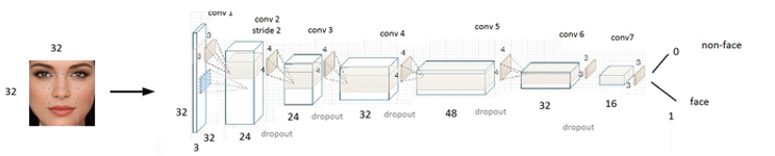
\includegraphics[width=1.0\textwidth]{image2-14}
  \caption{نمای کلی یک شبکه عصبی پیچشی برای یافتن چهره \cite{ref1}.}
  \label{image2-14}
\end{figure}

\noindent
با توجه به آنچه در \cite{8253595} آمده است، چالش اصلی در یافتن چهره این است که ویژگی‌هایی مانند \lr{Haar} و \lr{HOG} اطلاعات برجسته چهره را در شرایط مختلف نما، نورپردازی، رنگ پوست، انسداد، استفاده از لوازم آرایشی و... استخراج نمی‌کنند. این محدودیت بیشتر به دلیل ویژگی‌های استفاده شده در طبقه‌بندها است. با پیشرفت‌های اخیر در رویکردهای یادگیری عمیق و در دسترس بودن پردازنده‌های گرافیکی، استفاده از شبکه‌های عصبی پیچشی عمیق برای استخراج ویژگی امکان پذیر شده است. ویژگی‌های عمیق به دست آمده به طور گسترده‌ای برای یافتن چهره استفاده می‌شود. با توجه به شکل 2-15 روش‌های مبتنی بر شبکه عصبی پیچشی عمیق برای یافتن چهره به دو زیر شاخه تقسیم می‌شود: رویکرد مبتنی بر ناحیه و رویکرد پنجره لغزان.

\begin{figure}[h]
\centering
  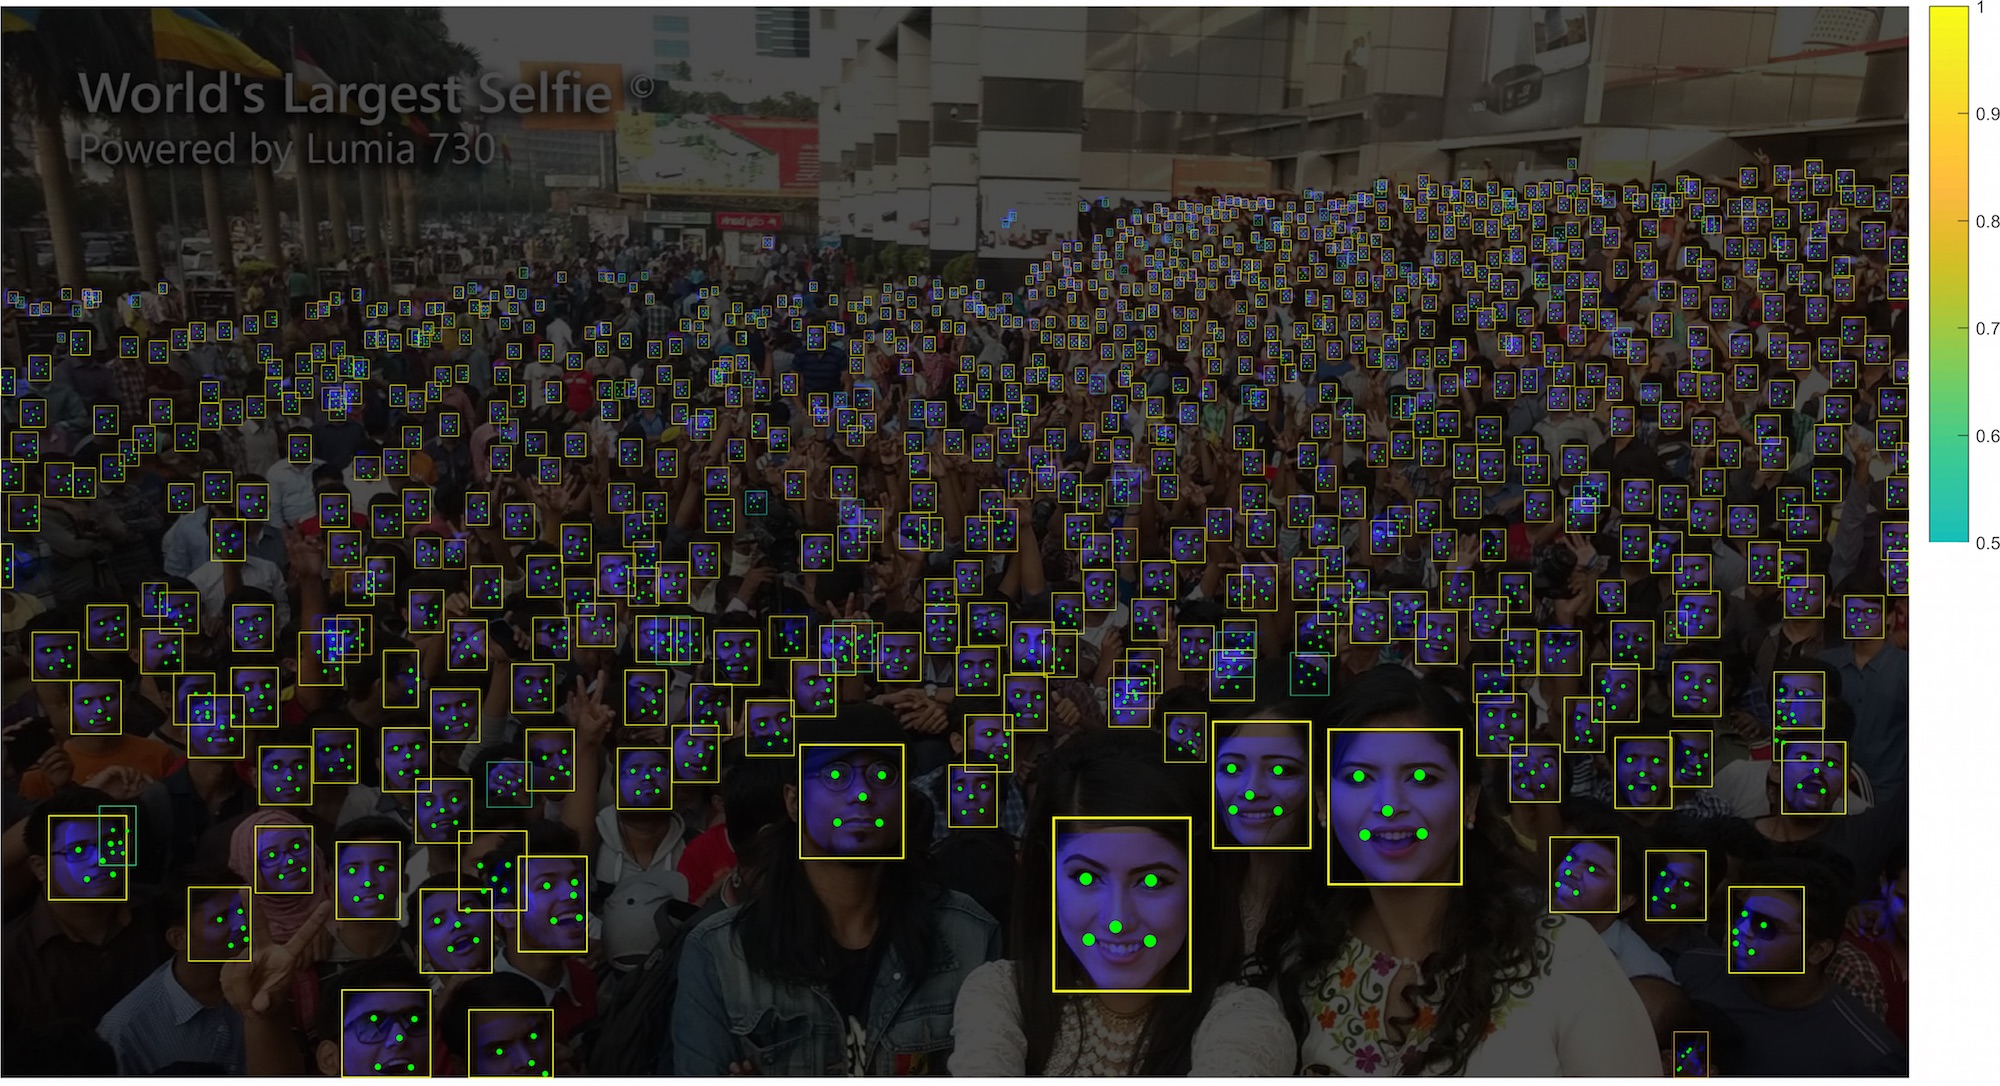
\includegraphics[width=1.0\textwidth]{image2-15}
  \caption{یافتن چهره مبتنی بر شبکه عصبی عمیق (a) رویکرد مبتنی بر ناحیه و (b) رویکرد پنجره لغزان \cite{ref1}.}
  \label{image2-15}
\end{figure}

\section{شناسایی چهره}
شناسایی چهره در دو مرحله انجام می‌شود. مرحله اول استخراج ویژگی و مرحله دوم، طبقه‌بندی است. الگوریتم‌های شناسایی چهره را می‌توان به دو دسته اصلی تقسیم کرد. الگوریتم‌های هندسی که بر مبنای استخراج ویژگی‌های متمایز چهره‌ها کار می‌کنند، و الگوریتم‌های تصویری که تصویر را تبدیل به یک الگو می‌نماید و الگوها را مقایسه می‌نماید. رویکردهای مختلفی برای شناسایی چهره طراحی شده است که در ادامه مهم‌ترین آن‌ها آمده است.

\subsection{رویکرد‌های سنتی}
این رویکردها ویژگی‌های چهره را با علامت‌ها و اندازه‌ها از تصویر استخراج می‌کنند. برای مثال موقعیت نسبی، اندازه و یا شکل چشم‌ها، بینی، گونه‌‌ها و فک را محاسبه کرده و تجزیه و تحلیل می‌کنند. سپس از این ویژگی‌ها برای جستجوی تصاویر دیگر در پایگاه داده استفاده می‌کنند. در سال 1993 \lr{Roberto Brunelli} و همکاران در \cite{254061} یکی از اولین الگوریتم‌ها در این زمینه را ارائه دادند که رویکرد‌ موفقی مبتنی بر روش‌های تطبیق الگو داشت (شکل 2-16). این رویکرد در شرایط کنترل شده به دقت 90\% رسید.
 
\begin{figure}[h]
\centering
  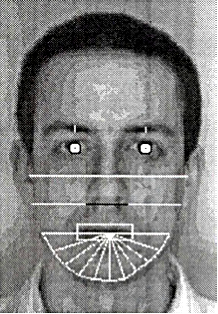
\includegraphics[scale=1]{image2-16}
  \caption{ویژگی های هندسی (رنگ سفید) مورد استفاده در آزمایش های تشخیص چهره \cite{ref1}.}
  \label{image2-16}
\end{figure}

\subsection{رویکرد مبتنی بر فیلتر گابور ‌}
همانطور که در \cite{ABATE20071885} آمده است، در این رویکرد ابتدا تصویر را بخش بندی \LTRfootnote{Grid} کرده، سپس بر روی بخش‌های مختلف آن، فیلتر گابور اعمال می‌شود و نتیجه بدست آمده با یک طرح از پیش آماده شده، با یک آستانه گذاری مطابقت داده می‌شود. شکل 2-17 فیلترهای چندگانه گابور \LTRfootnote{Gabor} و تاثیر این فیلترها بر روی تصویر چهره انسان را نشان می‌دهد. دلیل استفاده از فیلتر گابور این است که عملکرد این فیلتر به سامانه بصری انسان بسیار شباهت دارد. 
 	 
\begin{figure}
\begin{subfigure}{.5\textwidth}
  \centering
  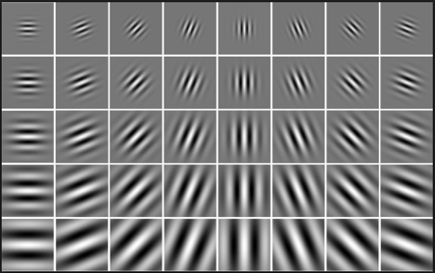
\includegraphics[width=1.0\textwidth]{image2-17-a}
  \label{image2-17-a}
\end{subfigure}
\begin{subfigure}{.5\textwidth}
  \centering
  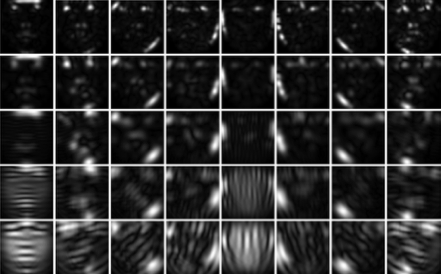
\includegraphics[width=1.0\textwidth]{image2-17-b}
  \label{image2-17-b}
\end{subfigure}
  \caption{(الف) فیلترهای چندگانه گابور (ب) تاثیر این فیلترها بر روی تصویر چهره \cite{ref1}.}
\label{fig:image2-17}
\end{figure}

\subsection{رویکرد‌های سه بعدی}
همانطور که در \cite{10.3745/JIPS.2009.5.2.041} آمده است، داده‌های سه بعدی دقت تشخیص چهره را به شدت بهبود می‌بخشد، اختلاف داده‌های ورودی با داده‌های ذخیره شده زیادتر است و سامانه با دقت بیشتری عمل می‌کند. روش تشخیص سه بعدی چهره از یک منتشر کننده نور فرو سرخ و یک حسگر به عنوان دریافت کننده استفاده می‌کند. شبکه‌ای از نورهای فرو سرخ که برای انسان قابل رویت نیست، روی چهره تابانده می‌شود. سپس یک حسگر ویژه، پرتوهای بازتاب را دریافت کرده و اطلاعات عمق تصویر پردازش می‌شود. این دسته از الگوریتم‌ها برای شناسایی دقیق اشخاص، برای هر نفر برداری‌های سه بعدی می‌سازند. عیب رویکردهای سه بعدی، نیاز به تجهیزات پیشرفته و غیر قابل استفاده بودن در شرایط کنترل نشده مانند خیابان و معابر پیاده می‌باشد. شکل 2-18 یک مدل سازی سه بعدی چهره با اشعه فروسرخ را نشان می‌دهد.

\begin{figure}[h]
\centering
  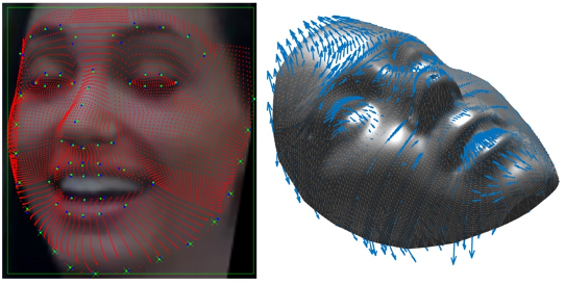
\includegraphics[scale=1]{image2-18}
  \caption{مدل سازی سه بعدی چهره با اشعه فرو سرخ \cite{ref1}.}
  \label{image2-15}
\end{figure}
 
 \subsection{رویکرد‌های تجزیه و تحلیل بافت پوست}
یکی دیگر از رویکردهای در حال ظهور، استفاده از بافت پوست برای شناسایی چهره می‌باشد که خطوط، الگوها و لکه-های پوست را به یک فضای ریاضی تبدیل می‌کند. تجزیه و تحلیل بافت بسیار شبیه روش شناسایی چهره است. تصویری از پوست گرفته می‌شود و به بخش‌های کوچکتر تقسیم می‌شود. سپس هر بخش به یک فضای ریاضی قابل اندازه گیری تبدیل می‌شود و خطوط، منافذ و بافت پوست تشخیص داده می‌شود. این رویکرد می‌تواند تفاوت بین دوقلوهای یکسان را شناسایی کند که با استفاده از تشخیص چهره به تنهایی امکان پذیر نیست. آزمایش‌ها نشان دادند که با افزودن تحلیل بافت پوست، عملکرد سامانه تشخیص چهره می‌تواند 20 تا 25 درصد افزایش یابد.

\noindent
در سال 2017 \lr{Guosheng Hu} و همکاران در \cite{HU2017366} یک روش سه بعدی برای توصیف ویژگی‌های چهره ارائه کردند که در آن از مدل سازی سه بعدی چهره به همراه تجزیه و تحلیل بافت پوست استفاده شده است. این سامانه شایستگی استفاده در کاربردهای مختلف امنیتی و نظامی با شناسایی خودکار سریع و بدون دخالت شخص را دارد و سرعت پردازش را بالا و خطا را کاهش داده است. برتری روش سه بعدی در عدم وابستگی به حرکت و جا به جایی صورت است. انتقال و نصب سامانه تصویر برداری بسیار ساده است. زاویه دید حسگر چندان مهم نیست. همچنین نورپردازی نامناسب تاثیری در این شیوه ندارد و عملیات آن ساده است.
بر خلاف روش تشخیص دو بعدی، روش سه بعدی و تجزیه و تحلیل بافت پوست به تجهیزات بسیار پیچیده تری نیاز دارد، و با توجه به آنکه تمرکز ما بر روی تشخیص چهره به صورت بی‌درنگ در شرایط کنترل نشده مانند معابر پیاده و خیابان می‌باشد، به توضیح مختصر رویکردهای سه بعدی و تجزیه و تحلیل بافت پوست بسنده می‌کنیم.

\subsection{رویکرد‌های مبتنی بر دوربین حرارتی}
در این رویکرد، دوربین حرارتی شکل صورت را تشخیص می‌دهد و از لوازم جانبی مانند عینک، کلاه یا آرایش چشم پوشی می‌کند. بر خلاف دوربین‌های معمولی، دوربین‌های حرارتی می‌توانند تصاویر را حتی در شرایط کم نور مانند شب، بدون استفاده از فلاش و قرار گرفتن در معرض مستقیم دوربین ضبط کنند. با این حال، یکی از مشکل‌های استفاده از تصاویر حرارتی برای تشخیص چهره این است که مجموعه داده‌های آن برای شناسایی چهره محدود است.

\noindent
در سال 2003 \lr{Diego Socolinsky} و همکاران در \cite{SOCOLINSKY200372} از شناسایی چهره مبتنی بر دوربین حرارتی در کاربردهای واقعی بهره برداری کردند و یک مجموعه داده جدید از تصاویر حرارتی چهره ایجاد کردند. آن‌ها از حسگرهای الکتریکی فروسرخ با حساسیت کم و با توانایی جذب حرارت طولانی مدت یا \lr{LWIR} \LTRfootnote{Longwave Infrared} استفاده کردند.
نتایج نشان می‌دهد که تلفیق \lr{LWIR} و دوربین‌های معمولی، نتایج بهتری در شرایط کنترل نشده دارد. در این مطالعه 240 چهره مجزا در طی 10 هفته برای ایجاد پایگاه داده جدید استفاده شده است. داده‌ها در روزهای آفتابی، بارانی و ابری جمع آوری شد. در شرایط کنترل شده دوربین معمولی دقت 97.05\% دارد، در حالی که روش \lr{LWIR} دارای دقت 93.93\% می‌باشد و ترکیب این دو دارای دقت 98.40\% است. در شرایط کنترل نشده دوربین معمولی دقت 67.06\%، دوربین \lr{LWIR} دقت 83.03\% و ترکیب این دو دارای دقت 89.02\% است.

\subsection{تشخیص چهره مبتنی بر ویدیو}
در سال 2009 \lr{Huafeng Wang} و همکاران در \cite{wang2009video} یک برآورد کلی از رویکردهای مبتنی بر ویدیو ارائه دادند. تشخیص چهره در ویدیو در طی چند سال گذشته مورد توجه قرار گرفته و طیف گسترده‌ای از برنامه‌های کاربردی تجاری و اجرای قانون را در بر گرفته است. فیلم‌ها قادر به ارائه اطلاعات بیشتر نسبت به تصاویر ثابت هستند. مزایای عمده استفاده از ویدیو عبارتند از:

\begin{enumerate}
\item
	امکان استفاده از افزونگی موجود در توالی ویدیو برای بهبود عملکرد تشخیص نسبت به تصاویر ثابت وجود دارد. تشخیص چهره و پیگیری آن در طول زمان، موجب انتخاب فریم‌های خوب می‌شود که حاوی چهره‌های رو به رو یا نشانه‌های ارزشمند است که شرایط نور، انسداد، حالت چهره و... در آن رضایت بخش می‌باشد.
\item 
	مطالعات روان پزشکی نشان داده است که اطلاعات پویا در فرایند تشخیص فرد بسیار حائز اهمیت است. 
\item
	نمایش‌های موثرتر مانند مدل چهره سه بعدی یا تصاویر \lr{super resolution} می‌توانند از اطلاعات فریم‌های ویدیو گرفته شده برای بهبود شناخت استفاده کنند.
\item
	یادگیری و به روز رسانی مدل در طول زمان امکان پذیر می‌باشد.
\end{enumerate}
	
\noindent
برای تشخیص چهره در تصاویر ویدیویی، دو رویکرد کلی وجود دارد:

\noindent
مبتنی بر قاب \LTRfootnote{Frame}: در این رویکرد برای شناسایی چهره، هر قاب به صورت جداگانه مورد پردازش قرار می‌گیرد که عیب آن نادیده گرفتن اطلاعات زمانی ارائه شده توسط توالی ویدیویی می‌باشد. 

\noindent
یافتن و ردیابی \LTRfootnote{Detection And Tracking}: یافتن چهره در اولین قاب و سپس ردیابی آن از طریق توالی قاب‌ها. شکل 2-19 نمای کلی این رویکرد را نشان می‌دهد.
 
 \begin{figure}[h]
\centering
  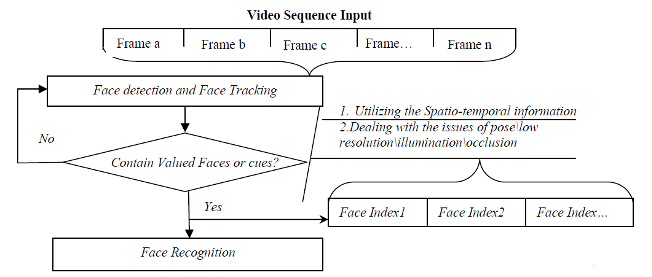
\includegraphics[width=1.0\textwidth]{image2-19}
  \caption{نمای کلی یک سامانه تشخیص چهره مبتنی بر ویدیو \cite{ref1}.}
  \label{image2-19}
\end{figure}

 \subsection{رویکرد مبتنی بر چهره ویژه}
با افزایش حجم داده‌های موجود، نیاز به کاهش ابعاد داده‌ها می‌باشد. تحلیل مؤلفه‌های اساسی یا \lr{PCA} \LTRfootnote{Principle Component Analysis} یک روش‌ کاهش ابعاد داده‌ها است که در برخی مسئله‌ها مانند پردازش تصویر به خوبی و با سرعت بالا عمل می‌کند. استفاده از این روش در پردازش سریع تر داده‌ها کمک می‌کند و از رخ دادن مشکل بیش‌برازاندن \LTRfootnote{Overfiting} جلوگیری می‌نماید. اگر یک پایگاه داده عظیم از تصاویر چهره اشخاص با وضوح بالا موجود باشد که هر کدام دارای تعدادی زیاد ویژگی هستند، و بخواهیم یک تصویر آزمایش را با این پایگاه داده مقایسه کرده و شخص شبیه به آن را پیدا کنیم، مقایسه تصاویر بسیار زمان بر و در مواردی غیر ممکن خواهد بود. \lr{PCA} در این مسئله به خوبی عمل می‌کند. با اعمال تکنیک کاهش بعد به تصویر و با به دست آوردن تصویر ویژه چهره‌ها \LTRfootnote{Eigenface} می‌توان ویژگی‌ها را کاهش داد و نتیجه مطلوب را در زمان بسیار کم گرفت. شکل 2-20 تعدادی چهره و چهره‌های ویژه متناظر با آن‌ها را نشان می‌دهد.

\noindent
در سال 2014 \lr{Xiao Luan} و همکاران در \cite{LUAN2014495} یک روش تشخیص چهره مبتنی بر \lr{PCA} ارائه دادند که تا حدی در برابر تغییرات نورپردازی و انسداد مقاوم می‌باشد. \lr{PCA} راستای بیشترین تغییرات را با توجه به تعداد ویژگی‌ها و نوع آن‌ها به ما می‌دهد. به همین دلیل در برخی موارد که تنها محوری که بیشترین تغییرات یا پراکندگی را دارد برای ما مهم است، راه حل مناسبی خواهد بود. 

\begin{figure}
\begin{subfigure}{.5\textwidth}
  \centering
  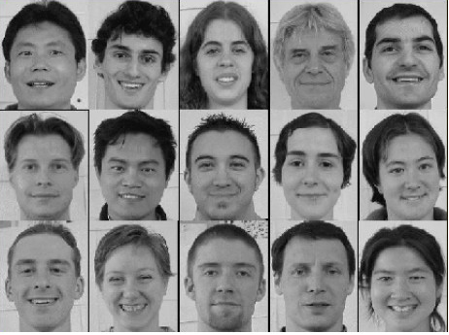
\includegraphics[width=1.0\textwidth]{image2-20-a}
  \label{image2-20-a}
\end{subfigure}
\begin{subfigure}{.5\textwidth}
  \centering
  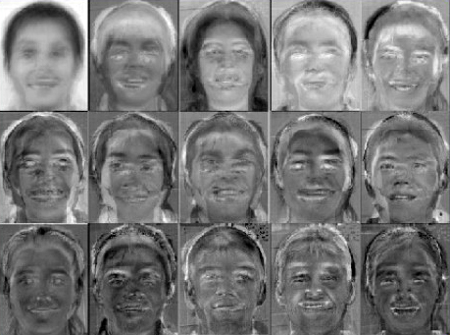
\includegraphics[width=1.0\textwidth]{image2-20-b}
  \label{image2-20-b}
\end{subfigure}
  \caption{ (الف) تعدادی چهره و (ب) چهره های ویژه متناظر با آن ها \cite{ref1}.}
\label{fig:image2-20}
\end{figure}

\noindent
در سال 2016 \lr{K. R. Sreelakshmi} و همکاران در \cite{7854053} یک روش شناسایی چهره مبتنی بر چهره‌های ویژه ارائه دادند که در آن ابتدا تصویر ورودی با استفاده از ماتریس بردارهای ویژه، به فضای دیگری منتقل می‎شود، سپس در فضای کاهش بعد یافته با داده‏های موجود مقایسه شده و شبیه‎ترین تصویر به آن انتخاب می‎شود. برای مقایسه از معیارهایی مانند معیار اقلیدسی و منهتن می‏توان استفاده کرد. از مزایای این روش می‏توان به سهولت پیاده‏سازی و استفاده، کاهش حجم داده‏ها و سرعت بالا اشاره کرد. در نظر نگرفتن پراکندگی درون کلاسی و بین کلاسی داده‏ها و عدم توجه به برچسب تصویر برای شناسایی و تمایز قایل نشدن بین تصاویر مختلف یک شخص در پایگاه و نیاز به بروز رسانی تمامی اطلاعات موجود با ورود یک تصویر جدید به پایگاه داده از معایب این روش است. 
محاسبات ریاضی و مراحل انجام آن‌ها:
\begin{enumerate}
\item
	تبدیل ماتریس تصاویر به بردار و کنار هم قرار دادن آن‌ها برای تشکیل ماتریس داده‏ها
\item 
	محاسبه‏ میانگین ماتریس بدست آمده و انتقال داده‏ها به مرکزیت صفر
\item
محاسبه‏ ماتریس کوواریانس بردارها و مقادیر ویژه‏ آن
\item
انتقال ماتریس داده‏ها به زیرفضای جدید با استفاده از ماتریس بردارهای ویژه
\item
	بررسی شباهت بین بردار منتقل شده و بردارهای موجود و انتخاب شبیه‏ترین بردار
\end{enumerate}

\subsection{رویکرد مبتنی بر ماشین بردار پشتیبان}
همان طور که در بخش 2-2-4-1 گفته شد، ماشین‌های بردار پشتیبان، طبقه‌بندهای خطی هستند که حاشیه بین ابرصفحه تصمیم و نمونه‌های مجموعه آموزش را به حداکثر می‌رسانند. در سال 2012 \lr{N.M.Khan} و همکاران در \cite{KHAN201266} این طبقه‌بند را برای تشخیص چهره مورد استفاده قرار دادند. یک نسخه مبتنی بر هسته برای \lr{SVM} معرفی شده که \lr{KSVM} نام گذاری شده است.

\begin{equation}\label{eq2-7}
a = b
\end{equation}

\noindent	
که در آن \lr{w} بردار وزن‌ها، \lr{x} داده‌های ورودی و \lr{w0} مقدار پیش قدر \LTRfootnote{Bias} می‌باشد. سپس یک مدل بی پارامتر از \lr{LDA} \LTRfootnote{Linear Discriminant Analysis} به نام \lr{NDA} \LTRfootnote{Nonparametric Discriminant Analysis} معرفی شده، سپس یک نسخه مبتنی بر هسته \LTRfootnote{Kernel} به نام \lr{KNDA} \LTRfootnote{Kernel Nonparametric Discriminant Analysis} معرفی شده است. 

\begin{equation}\label{eq2-8}
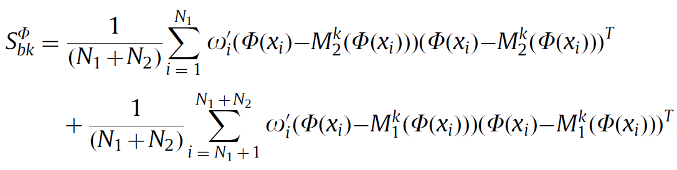
\includegraphics[height=3cm]{equation2-8}
\end{equation}

\noindent
که در آن \lr{N1} و \lr{N2} تعداد نمونه‌های آموزشی در هر دسته می‌باشند. سپس از ترکیب دو رویکرد فوق، مدلی به نام \lr{SVM + NDA} طراحی نموده است. 
\begin{equation}\label{eq2-9}
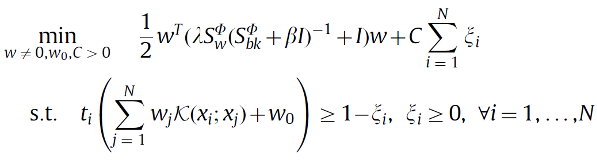
\includegraphics[height=3cm]{equation2-9}
\end{equation}	

\noindent
که در آن \lr{βI} ماتریس تنظیم می‌باشد و \lr{λ} ضریبی برای تنظیم کنترل میان \lr{SVM} و \lr{NDA} می‌باشد. رابطه بالا یک مسئله بهینه سازی می‌باشد که به صورت تکراری قابل حل ‌می‌باشد. دقت این روش در مقایسه با سایر روش‌های مشابه در جدول 2-1 آورده شده است.

\begin{table}
  \caption{ مقایسه دقت الگوریتم SVM + NDA با سایر رویکرد های مشابه}
  \label{tbl:2-1}
  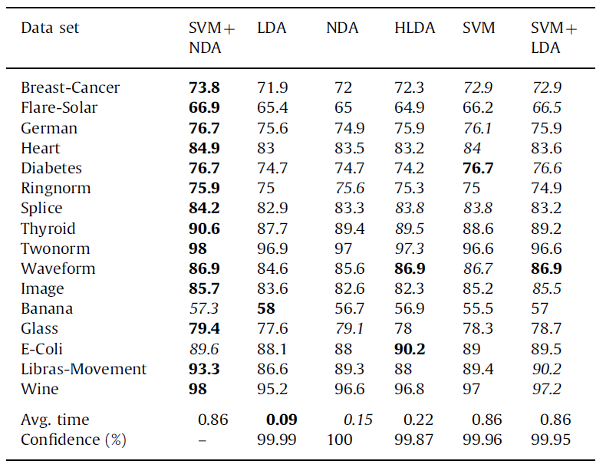
\includegraphics[width=\linewidth]{table2-1}
\end{table}
 
\subsection{رویکردهای مبتنی بر شبکه عصبی}
یک راه حل غیر خطی برای شناسایی چهره، استفاده از شبکه‌ عصبی پیچشی است که به طور شگفت انگیزی در طبقه-بندی تصاویر چهره خوب کار می‌کند و ویژگی‌های ارزشمندی را از تصویر چهره استخراج می‌کند. بنابراین می‌توان از آن در حل مسئله شناسایی چهره‌ و تأیید هویت استفاده کرد. شکل 2-21 ساختار کلی یک شبکه عصبی عمیق برای شناسایی چهره را نشان می‌دهد.
 
\begin{figure}[h]
\centering
  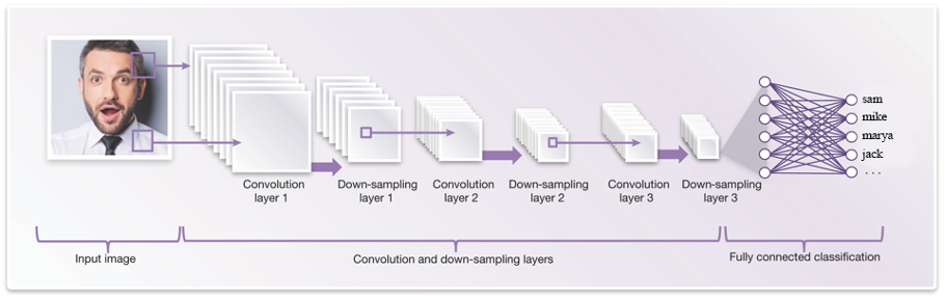
\includegraphics[width=1.0\textwidth]{image2-21}
  \caption{شبکه عصبی عمیق برای شناسایی چهره \cite{ref1}.}
  \label{image2-21}
\end{figure}

\noindent
معمولا به عنوان تابع فعالیت از توابع غیرخطی مانند \lr{ReLU} \LTRfootnote{Rectified Linear Unit} استفاده می‌شود. و عملیات بهینه سازی به روش پس انتشار خطا انجام می گردد. و در لایه خروجی از تابع \lr{SoftMax} برای طبقه‌بندی استفاده می‌شود که خروجی های لایه آخر را هنجار می‌کند. شبکه‌های عصبی پیچشی ویژگی‌های یک چهره را استخراج می‌کنند که می‌توان به عنوان یک شناسه برای یک فرد خاص در نظر گرفت. هنگامی که دو تصویر مختلف از چهره یک شخص به عنوان ورودی داده می‌شود، شبکه باید خروجی‌های مشابه (ویژگی‌های نزدیک تر) را برای هر دو تصویر تولید نماید، در حالی که برای چهره دو شخص مختلف، شبکه باید خروجی‌های بسیار متفاوت برای دو تصویر تولید نماید. شبکه عصبی نیاز به آموزش دارد تا به طور خودکار ویژگی‌های مختلف چهره‌ها را شناسایی کند و بر اساس آن محاسبات را انجام دهد. در ادامه چند شبکه عصبی پیچشی معروف مورد بررسی قرار گرفته است.

\subsubsection{	شبکه \lr{FaceNet}}
در سال 2015 \lr{Florian Schroff} و همکاران در \cite{7298682} یک شبکه عصبی عمیق به نام \lr{FaceNet} ارائه دادند. \lr{FaceNet} یک مدل یکپارچه است که می‌آموزد چگونه تصاویر چهره را به یک فضای اقلیدسی فشرده نگاشت دهد تا فاصله تصاویر به طور مستقیم با میزان شباهت چهره‌ها مرتبط باشد. هنگامی که این فضا تولید شود، شناسایی چهره، تایید هویت و خوشه‌بندی می‌تواند به راحتی با استفاده از روش‌های استاندارد توسط \lr{FaceNet} انجام شود. این شبکه برای آموزش از سه گانه تطبیق – عدم تطبیق استفاده می‌نماید. با توجه به شکل 2-22، سه گانه تطبیق – عدم تطبیق یک مجموعه از سه تصویر شامل یک تصویر مرجع، یک تصویر منطبق بر تصویر مرجع و یک تصویر غیر منطبق بر تصویر مرجع است که باید فاصله بین تصویر مرجع و تصویر منطبق را به حداقل برساند، زیرا هر دو دارای هویت مشابه هستند و فاصله بین تصویر مرجع و تصویر غیر منطبق را به حداکثر برساند، زیرا این تصاویر دارای هویت متفاوت می‌باشند. 
 
 \begin{figure}[h]
\centering
  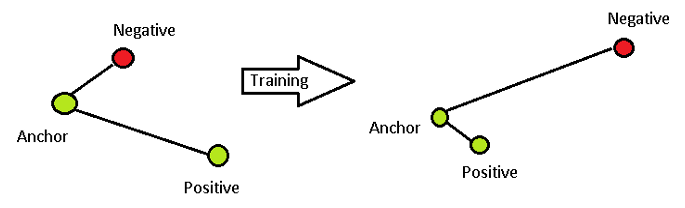
\includegraphics[width=0.5\textwidth]{image2-22}
  \caption{سه گانه تطبیق – عدم تطبیق \cite{ref1}.}
  \label{image2-22}
\end{figure}

\noindent 
برای هر داده آموزشی \lr{A} مجموعه‌ای از داده‌های مشابه \lr{Positive} و مجموعه‌ای از داده‌های نامرتبط \lr{Negative} در نظر گرفته می‌شود. سپس داده‌ها با تابع ضرر سه گانه طوری آموزش می‌بینند که رابطه زیر برای هر کدام از داده‌های آموزشی برقرار باشد.
\begin{equation}\label{eq2-10}
‖f(A)-f(P)‖^2≤‖f(A)-f(N)‖^2	
\end{equation}

\noindent
که در آن تابع \lr{𝑓} ویژگی‌های استخراج شده از تصاویر است. شبكه در مرحله آموزش با استفاده از داده‌های برچسب‌گذاری شده، می‌آموزد فاصله بین ویژگی‌های شبیه به هم، کمتر از فاصله بین ویژگی‌های دور باشد و به این ترتیب در مرحله آزمایش می‌تواند داده‌های مشابه و غیر مشابه را به راحتی تفكیک نماید. تابع هزینه در این مدل برای هر نمونه آموزشی 𝑥𝑖  به صورت زیر تعریف می‌شود:
\begin{equation}\label{eq2-11}
L=∑_(i=1)^n▒〖‖f(x_i^A )-f(x_i^P)‖^2-‖f(x_i^A )-f(x_i^N)‖^2 〗+α	
\end{equation}

\noindent
که در آن
x\textsubscript{i}\textsuperscript{P}   
و
x\textsubscript{i}\textsuperscript{N}   
نمونه های مثبت و منفی برای نمونه آموزشی
x\textsubscript{i}\textsuperscript{A}
می‌باشند و \lr{α} حاشیه بین داده‌های مثبت و منفی را برای هر داده آموزشی مشخص می‌کند. این شبکه در مجموعه داده برچسب دار \lr{LFW} به دقت جدید 99.63\% رسیده است و در مجموعه داده
\lr{YouTube Faces DB}
دقت آن به 95.12\% رسیده است.
	
\subsubsection{	شبکه \lr{SplitNet}}
در سال 2018 Wen و همکاران در \cite{WEN201894} یک شبکه عمیق به نام \lr{SplitNet} برای شناسایی چهره ارائه دادند. با توجه به ساختار معنایی چهره، یک بخش محلی از تصویر چهره همانند تصویر کلی چهره حاوی ویژگی‌ها و اطلاعات مفیدی برای یادگیری عمیق است. به منظور استفاده همزمان از اطلاعات سراسری و محلی، روش‌های یادگیری عمیق موجود برای شناسایی چهره، چندین شبکه CNN را آموزش می‌دهند و ویژگی‌های مختلف را بر اساس مکان تصاویر محلی ترکیب می‌کنند که نیاز به عملیات متعدد و محاسبات بسیار بیشتری برای هر تصویر دارد. هدف این مقاله بهبود تشخیص چهره تنها با یک عملیات پیشخور \LTRfootnote{Feed Forward} است که به طور همزمان از اطلاعات سراسری و محلی در یک مدل استفاده می‌کند. آن‌ها یک چارچوب یکپارچه به نام \lr{SplitNet} ارائه دادند که به جای آن که تصویر اصلی را برش دهد، ویژگی‌های میانی را به چندین شاخه تقسیم می‌کند. شکل ‏2-23 شبکه عصبی پیچشی \lr{SplitNet} را در مقابل شبکه عصبی پیچشی معمولی نشان می‌دهد. نتایج تجربی نشان می‌دهد که این رویکرد می‌تواند به طور موثر دقت تشخیص چهره را با محاسبات کمتر افزایش دهد. 
 	 
\begin{figure}
\begin{subfigure}{.5\textwidth}
  \centering
  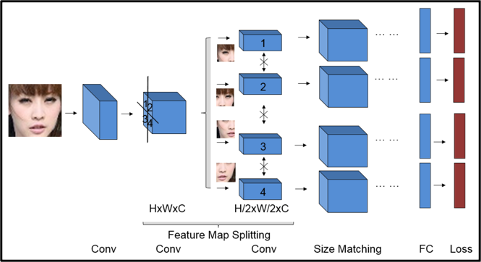
\includegraphics[width=1.0\textwidth]{image2-23-a}
  \label{image2-23-a}
\end{subfigure}
\begin{subfigure}{.5\textwidth}
  \centering
  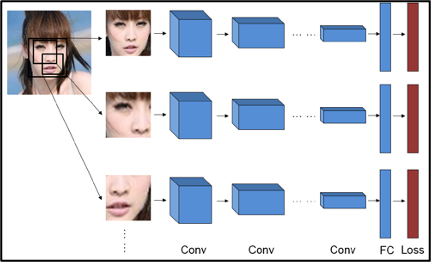
\includegraphics[width=1.0\textwidth]{image2-23-b}
  \label{image2-23-b}
\end{subfigure}
  \caption{ (الف) شبکه عصبی پیچشی \lr{SplitNet}  (ب) شبکه عصبی پیچشی معمولی \cite{ref1}.}
\label{fig:image2-23}
\end{figure}

\subsubsection{	شبکه \lr{GoogLeNet}}
در سال 2015 \lr{Christian Szegedy} و همکاران در \cite{7298594} یک شبکه عصبی عمیق به نام \lr{GoogLeNet} ارائه دادند. همانطور که در شکل 2-24 مشاهده می‌شود، \lr{GoogLeNet} یک شبکه عصبی پیچشی با 22 لایه است که یکی از اولین معماری های شبکه عصبی پیچشی بود که از رویکرد کلی قرار دادن تعداد زیادی از لایه‌های پیچشی و رای گیری  در کنار هم در یک ساختار متوالی بدست آمد. نویسندگان این مقاله همچنین تأکید کردند که این مدل جدید، توجه قابل ملاحظه ای به مصرف حافظه و مصرف انرژی دارد، زیرا کنار هم چیدن تعداد زیادی لایه و فیلتر دارای هزینه محاسباتی و حافظه است که احتمال بيش‌برازاندن  را افزایش می‌دهد.
 
\begin{figure}[h]
\centering
  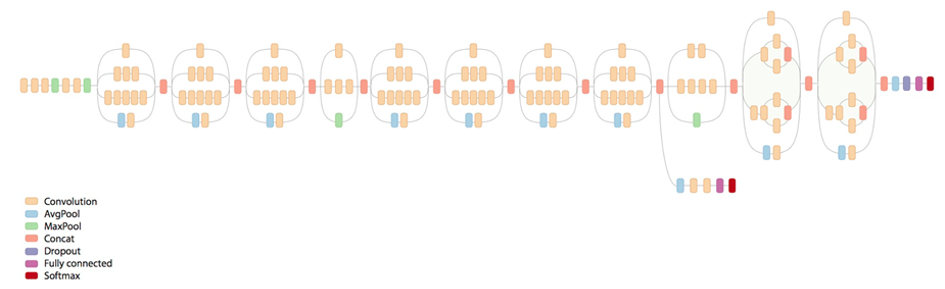
\includegraphics[width=1.0\textwidth]{image2-24}
  \caption{معماری کلی شبکه \lr{GoogLeNet} \cite{ref1}.}
  \label{image2-24}
\end{figure}

\noindent
در \lr{GoogLeNet} تمام محاسبات به طور متوالی اتفاق نمی‌افتد، بلکه هر بخش شبکه روندی موازی دارد. کادر سبز رنگ در شکل 2-25 بخش آغازگر نامیده می‌شود. در ادامه نگاهی دقیق تر به این بخش خواهیم داشت.
 
\begin{figure}[h]
\centering
  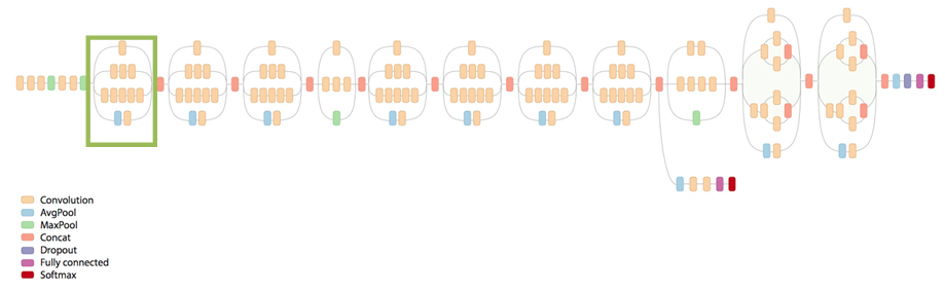
\includegraphics[width=1.0\textwidth]{image2-25}
  \caption{کادر سبز رنگ یکی از بخش های موازی شبکه را نشان می دهد \cite{ref1}.}
  \label{image2-25}
\end{figure}

\noindent
کادر سبز پایین در شکل 2-26 ورودی این بخش و کادر بالایی خروجی می‌باشد. در هر لایه شبکه‌های پیچشی معمولی، باید بین یک لایه پیچشی یا رای گیر، یکی را انتخاب نمود. در حالی که اینجا می‌توان تمام این عملیات را به صورت موازی انجام داد. این همان ایده ساده ای بود که نویسندگان مقاله روی آن تمرکز کردند.
 
\begin{figure}[h]
\centering
  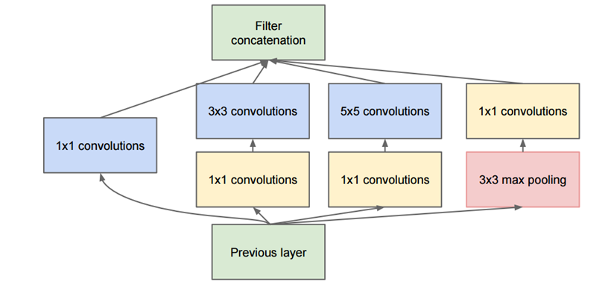
\includegraphics[scale=1]{image2-26}
  \caption{بخش آغازگر شبکه \lr{GoogLeNet} \cite{ref1}.}
  \label{image2-26}
\end{figure}

\subsubsection{	شبکه \lr{VGGFace}}
در سال 2015 \lr{Omkar M. Parkhi} و همکاران در \cite{parkhi2015deep} شبکه عمیق \lr{VGGFace} را ارائه کردند که شامل یک توالی طولانی از لایه‌های پیچشی می‌باشد. با توجه به شکل 2-27 این شبکه که در لایه آخر به عنوان یک طبقه‌بند عمل می‌نماید، هر تصویر آموزشی چهره را توسط لایه تماما متصل و تابع ضرر \lr{softmax log-loss} به یک بردار تبدیل می‌نماید که هر مقدار در این بردار، نشان دهنده احتمال برای یک هویت فردی است. \lr{VGGFace} مشابه \lr{FaceNet} از یک تابع ضرر سه گانه \LTRfootnote{Triplet Loss Function} در آموزش برای بهبود عملکرد کلی استفاده می‌نماید.
 
 \begin{figure}[h]
\centering
  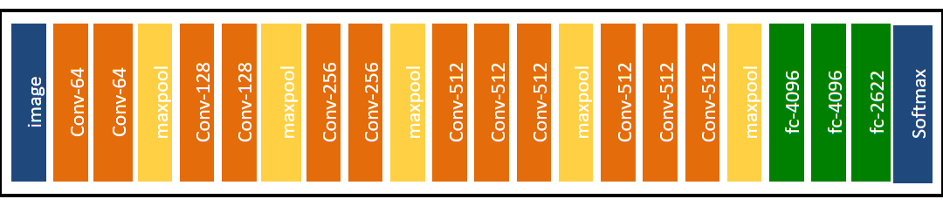
\includegraphics[width=1.0\textwidth]{image2-27}
  \caption{معماری شبکه \lr{VGGFace} \cite{ref1}.}
  \label{image2-27}
\end{figure}

 \subsection{رویکردهای مبتنی بر نقاط راهنما} 
چهره‌هايى كه در جهت‌هاى مختلفى هستند، براى سامانه تشخیص چهره، متفاوت به نظر مي‌رسند. براى غلبه بر اين چالش در رویکردهای مبتنی بر نقاط راهنما سعى مي‌شود تصوير را چرخانده و جابه جا نمود، بطوريكه چشم‌ها و لب‌ها در يك موقعيت خاص در تصوير قرار بگیرند. بدین ترتیب مقايسه چهره‌ها در مرحله بعد بسيار ساده‌تر خواهد شد.

\noindent 
در سال 2014 وحيد كاظمى و جوزفين ساليوان در \cite{6909637} یک الگوریتم برای یافتن نقاط راهنما \LTRfootnote{Landmark} بر روی چهره ارائه دادند كه از 194 نقطه خاص كه در هر چهره اى وجود دارد استفاده مي‌نماید. شکل 2-28 مکان این نقاط را بر روی گونه، لبه-هاى بیرونی چشم، كناره ابرو و... نشان می‌دهد. سپس اين 194 نقطه به سامانه آموزش داده می‌شود تا در هر چهره‌اى آن-ها را تشخيص دهد. 
\begin{figure}[h]
\centering
  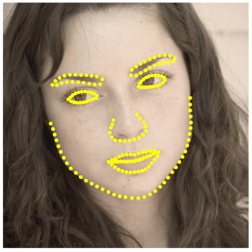
\includegraphics[scale=1]{image2-28}
  \caption{نتیجه موقعیت 194 شاخص روی چهره \cite{ref1}.}
  \label{image2-28}
\end{figure}
\noindent
پس از این که دانستیم چشم‌ها، دهان و ... کجاست، به راحتی می‌توانیم تناسب تصویر را تغییر داده و آن را چرخانده یا برش بزنیم. به طوری که چشم‌ها و دهان در بهترین حالت ممکن در مرکز قرار گیرد. با استفاده از تغییرات اساسی و اصلی تصویر، مانند تغییر اندازه، چرخش، خطوط موازی را حفظ می‌کنیم که در ریاضی به آن تغییرات نسبت یا افاین می‌گویند. شکل 2-29 علامت گذاری تکراری خطوط راهنما بر روی چهره را نشان می‌دهد. 
\begin{figure}[h]
\centering
  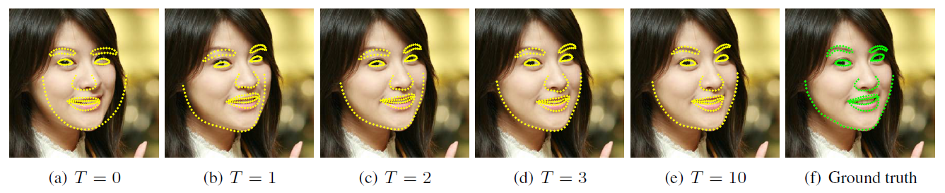
\includegraphics[width=1.0\textwidth]{image2-29}
  \caption{علامت گذاری خطوط راهنما بر روی چهره که در هر تکرار با کاهش خطا همراه می باشد \cite{ref1}.}
  \label{image2-29}
\end{figure}

\noindent
در سال 2016 \lr{Yue Wu} و همکاران در \cite{wu2016facial} رویکردی برای یافتن نقاط راهنما بر روی چهره مبتنی بر شبکه عصبی پیچشی ارائه دادند. در این مقاله یک معماری جدید برای شبکه عصبی پیچشی به نام
\lr{Tweaked CNN}
پیشنهاد شده است که به اختصار \lr{TCNN} نامیده می‌شود. این شبکه عصبی عمیق از 4 لایه پیچشی ($CL_1 \dots CL_4$) با لایه‌های رای‌گیری در میان آن‌ها تشکیل شده است و در انتهای یک لایه تمام متصل  $FC_5$ و پس از آن یک لایه خروجی با اندازه $2*m$ آمده است که مختصات m نقطه ویژه را بر روی چهره مشخص می‌کند. در این مقاله m برابر با 5 در نظر گرفته شده است. تابع فعالیت برای هریک از لایه‌های پیچشی $f(x)=|tanh⁡(x)|$ و تابع فعالیت برای لایه تمام متصل $f(x)=tanh⁡(x)$ در نظر گرفته شده است. و در نهایت تابع زیر به عنوان تابع ضرر معرفی شده است.
\begin{equation}\label{eq2-12}
L(P_i,\hat{P_i})=\frac{(‖P_i-P ̂_i ‖_2^2)}{(‖P ̂_(i,1)-P ̂_(i,2) ‖_2^2 )}	
\end{equation}
\noindent
که در آن $P_i$ یک بردار $2*m$ برای مختصات پیش بینی شده تصویر $I_i$ و $P_i$ و مختصات محل دقیق آن نقاط می‌باشد. $P_{i,1}$ و $P_{i,2}$ مختصات چشم ها در تصویر مرجع می‌باشند. در نهایت خروجی لایه تمام متصل توسط الگوریتم \lr{GMM} به 64 خوشه تقسیم شده و هریک به صورت جداگانه بررسی شده است. معماری \lr{TCNN} در شکل 2-30 قسمت b قابل مشاهده می‌باشد. این شبکه برای آموزش از مجموعه داده \lr{LFW} استفاده کرده است.

\begin{figure}[h]
\centering
  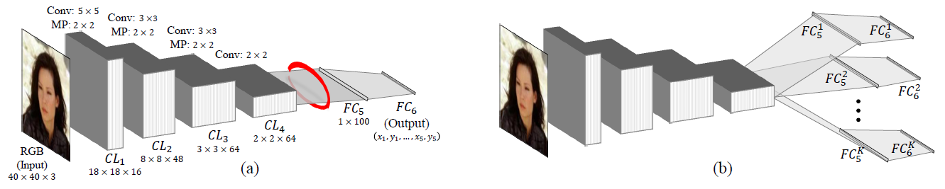
\includegraphics[width=1.0\textwidth]{image2-30}
  \caption{(a) شبکه عصبی پیچشی معمولی و (b) شبکه عصبی پیچشی با معماری \lr{TCNN} \cite{ref1}.}
  \label{image2-30}
\end{figure}
\noindent
در سال‌های بعد شبکه‌های عمیق‌تر، پهن‌تر و البته پیچیده‌تر مانند GoogleNet ResNet ResNext و... برای رسیدن به دقت بالاتر مطرح شد. باوجود پیچیدگی در طراحی این شبکه‌ها، تمرکز اصلی ‌بر روی دقت بود و جای خالی شبکه‌های با سایز کوچک و سرعت بالا با قابلیت استفاده در رباتیک، بردهای مینی‌کامپیوتری و البته موبایل‌ها احساس می‌شد که ایده دسته جدیدی از شبکه‌های کانولوشنی سبک با پارامترهای کم‌ شکل گرفت. یکی از شاخص‌ترین شبکه‌های سبک، شبکه عصبی MobileNet نام دارد که توسط محققان گوگل با هدف طراحی شبکه‌های کارآمد، سبک، سریع و با دقت قابل‌قبول مطرح شده است. در سال ۲۰۱۹ Andrew Howard و همکاران در \cite{howard2019searching} معماری MobileNet نسخه ۳ را ارائه دادند. در این مقاله یک نوع کانولوشن جدید به‌نام depth-wise separable convolution معرفی شد که قلب تپنده شبکه موبایل نت است. در کانولوشن dws ابتدا کانولوشن عمقی اعمال می‌شود و سپس کانولوشن نقطه‌ای که به‌ترتیب نقش مراحل فیلتر و ادغام در کانولوشن استاندارد را دارند. در کانولوشن استاندارد M کرنل k×k داشتیم. اما در اینجا تنها یک کرنل k×k داریم! حالا با این کرنل، مرحله اول کانولوشن را انجام می‌دهیم. با انجام عمل فیلتر، هرصفحه از کرنل در یک صفحه از فیچرمپ ورودی F کانوالو می‌شود. به این مرحله کانولوشن عمقی گفته می‌شود. 
مرحله دوم، کانولوشن نقطه‌ای (point-wise) هست. این مرحله معادل با مرحله ادغام در کانولوشن استاندارد است. اما بازهم یک تفاوت اساسی بین مرحله ادغام در کانولوشن استاندارد و کانولوشن dws وجود دارد:
مرحله ادغام در کانولوشن استاندارد، یک جمع ساده هست، اما مرحله ادغام در کانولوشن dws شامل یک کانولوشن 1×1 است.
کانولوشن نقطه‌ای همان کانولوشن استاندارد یا رایجی هست که می‌شناسیم و در بسیاری از شبکه‌های کانولوشنی استفاده می‌شود. این کانولوشن 1×1 وظیفه مهمی دارد؛ کانولوشن نقطه‌ای 1×1 خروجی‌های کانولوشن عمقی (مرحله اول) را با هم ادغام می‌کند. در مرحله قبل بجای تعریف M کرنل، تنها یک کرنل تعریف کردیم. اما در این مرحله، M کرنل 1×1 تعریف می‌کنیم.

\begin{figure}[h]
\centering
  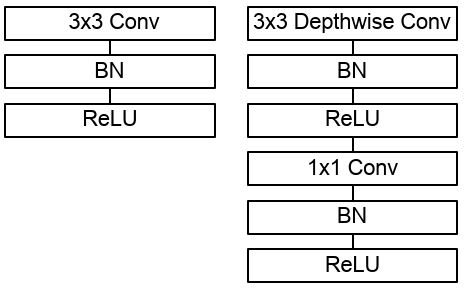
\includegraphics[width=0.5\textwidth]{image2-31}
  \caption{
  کانولوشن استاندارد (سمت چپ). کانولوشن dws که شامل دو کانولوشن depth-wise و point-wise هست (سمت راست). 
   \cite{ref1}.}
  \label{image2-31}
\end{figure}
\noindent
شبکه عصبی موبایل نت 4.2 میلیون پارامتر دارد. وقتی تعداد پارامترهای این شبکه را با شبکه محبوب ResNet-18 با 11 میلیون پارامتر مقایسه کنیم، متوجه می‌شوید که چقدر میزان پارامترها کمتر است.
\begin{table}
\centering
  \caption{ مقایسه شبکه عصبی موبایل نت با گوگل نت و VGG.}
  \label{tbl:2-2}
  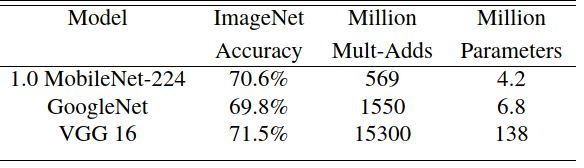
\includegraphics[width=0.5\textwidth]{table2-2}
\end{table}

در سال ۲۰۲۱ yang و همکاران در \cite{yang2021sanet} یک ماژول مبتنی بر لایه توجه ارائه دادند. لایه‌های توجه که یک شبکه عصبی را قادر می‌سازد تا دقیقاً بر روی تمام عناصر مربوط به ورودی متمرکز شود، به یک جز اساسی برای بهبود عملکرد شبکه‌های عصبی عمیق تبدیل شده است. عمدتا دو مکانیسم توجه به طور گسترده در بینایی رایانه مورد استفاده قرار می گیرد: لایه توجه وابسته به كانال \LTRfootnote{Channel Attention Module} و لایه توجه وابسته به موقعيت \LTRfootnote{Spatial Attention Module} که به ترتیب به منظور توجه به رابطه دو به دو در سطح کانال و در سطح پیکسل هستند. اگرچه تلفیق آن‌ها ممکن است عملکرد بهتری نسبت به پیاده سازی های منفرد آنها به دست آورد‌، اما سربار محاسباتی را افزایش می‌دهد.
در این مقاله، یک ماژول Shuffle Attention (SA) کارآمد برای پرداختن به این مسئله پیشنهاد شده است. SA ابتدا ابعاد کانال را به چندین ویژگی فرعی قبل از پردازش موازی آنها تقسیم می‌کند. سپس، برای هر زیر ویژگی از یک واحد Shuffle برای به تصویر کشیدن وابستگی های ویژگی در هر دو بعد مکانی و کانال استفاده می‌کند. پس از آن ، همه زیر ویژگی ها جمع می شوند و یک عملگر تغییر کانال برای امکان برقراری ارتباط اطلاعاتی بین ویژگی های فرعی مختلف به کار گرفته می شود. معماری این ماژول در شکل \ref{image2-32} آمده است.
\begin{figure}[h]
\centering
  \includegraphics[width=1\textwidth]{image2-32}
  \caption{
  معماری ماژول Shuffle Attention
   \cite{yang2021sanet}.}
  \label{image2-32}
\end{figure}
\noindent
ماژول SA بهینه و در عین حال کارآمد است ، به عنوان مثال، پارامترها و محاسبات SA در شبکه ResNet50 به ترتیب 300 در مقابل 25.56 میلیون است، اما افزایش عملکرد بیش از 1.34٪ را به ارمغان می‌آورد. نتایج تجربی نشان می‌دهد که SA برای دستیابی به دقت بالاتر مناسب است، در حالی که دارای پیچیدگی مدل کمتری است و از روش های SOTA \LTRfootnote{State of the Art} کنونی به مراتب بهتر عمل می‌کند. 

\section{نتیجه گیری}
در این فصل مفاهیم‌ پایه در مبحث یافتن و تشخیص چهره در تصاویر و انواع الگوریتم‌های دسته ‌بندی از روی تصاویر رنگی بررسی شد. همانطور که در قبل نیز بیان شد، برای حل مساله دسته ‌بندی چهره دو روش کلی، مبتنی بر تصویر و روش‌های مبتنی بر استخراج ویژگی وجود دارد. همچنین روش‌های مبتنی بر تصویر خود دارای رویکردهای مختلفی از جمله روش‌های مبتنی بر رنگ‌ بندی، روش‌های مبتنی بر شکل و روش‌های مبتنی بر گرادیان می‌باشد: همچنین روش های مبتنی بر استخراج ویژگی که در سال های اخیر بسیار مورد توجه قرار گرفته اند شامل رویکردهای مبتنی بر شبکه عصبی، بردار پشتیبان و... می باشند.

با بررسی شبکه‌های به‌روز از جمله MobileNetV2، MobileNet, NASNetMobile، SqueezeNet، VGG19، ResNet-50، و EfficientNetB0
و مقایسه دقت و زمان پاسخگویی آن‌ها به کمک یادگیری انتقال، به این نتیجه می‌رسیم که شبکه های MobileNetV2 و SqueezeNet دارای چگالی دقت بالاتری می‌باشند و نسبت دقت دسته بندی به تعداد پارامترهای شبکه در آن‌ها بیشتر می‌باشد. بنابرین می‌توان سرعت اجرای مناسب و همچنین دقت مناسب را از آن‌ها انتظار داشت. نتایج بررسی در شکل \ref{image2-33} آمده اند.

\begin{figure}[h]
\centering
  \includegraphics[width=0.5\textwidth]{image2-33}
  \caption{
  مقایسه چگالی دقت در معماری‌های مختلف شبکه عصبی پیچشی 
   \cite{Bianco_2018}.}
  \label{image2-33}
\end{figure}
\chapter{مروری بر کارهای گذشته در شرایط کنترل نشده}
\section{مقدمه}
در سال های اخیر روش های تشخیص چهره بسیار زیادی به منظور یافتن و شناسایی چهره افراد در تصویر پیشنهاد شده است که توانایی مقاومت در برابر مشکلات و چالش های رایج مانند تغییرات شدید روشنایی، تغییر حالت و زاویه چهره، انسداد ، تاری خارج از تمرکز، سالخوردگی و... را ندارند و در کاربردهایی نظیر شرایط کنترل نشده قابل استفاده نیستند. در بخش مقدمه در مورد چالش های موجود در فرایند تشخیص چهره صحبت شد. برای رفع این چالش ها و بهبود طبقه بندی، راه حل هایی پیشنهاد شده است که در این بخش مورد بررسی قرار گرفته اند.
جدول \ref{table:3-1} خلاصه ای از روش های مقابله با شرایط کنترل نشده

\begin{table}[ht]
\label{table:3-1}
\begin{center}
\resizebox{\textwidth}{!}
{
\begin{tabular}{|c|c|c|c|c|}
\hline 
مقاله ها & چالش مورد نظر & رویکرد & مزیت ها & مشکل ها
\\
\hline 
\cite{HAGHIGHAT201623, LV2016465, amos2016openface, 6196234}
& حالت چهره	 & تبدیل دوبعدی & 	پیچیدگی محاسباتی قابل قبول & 	استخراج نقاط ویژه باید دقیق تر باشد
 \\
\hline
\cite{wu2016facial, 7477555, 7780892, 7532959, 7298667}
 & حالت چهره & 	استفاده از شبکه عصبی عمیق & دقت بالا در شرایط کنترل نشده & 	پیچیدگی محاسباتی، وابستگی به داده های آموزش 
\\
\hline
\cite{HU2017366, hassner2014effective, 7298679, 7006757, 6905796}
 & حالت چهره & 	تبدیل مدل دو بعدی به سه بعدی & 	دقت بالا 	پیچیدگی محاسباتی &
\\
\hline 
\cite{DING2017144}
& حالت چهره & 	تبدیل مدل سه بعدی به دو بعدی & 	دقت بالا 	پیچیدگی محاسباتی &
\\
\hline
\cite{6196234, HUSSAINSHAH201597}
 & روشنایی	 & همسان سازی بافت-نگار & 	پیچیدگی محاسباتی قابل قبول & 	قابل استفاده در تصاویر خاکستری
\\
\hline
\cite{7015448, WU2018256}
 & انسداد	 & استفاده از روش های شناسایی الگو و وایازش & 	دقت بالا در انسداد شدید &	
\\
\hline
\cite{7984553}
 & محدودیت داده	 & تهیه مجموعه داده با ردیابی چهره در ویدیو & 	تهیه مجموعه داده با دقت بالا & 	نیاز به یک مرحله طولانی استفاده از تصاویر ویدیو
\\
\hline
\cite{6249269, HU2018582}
 & محدودیت منابع & 	استفاده از رایانش ابری & 	سرعت بالا & 	تجهیزات پیشرفته و زمان تاخیر ناهمگن
\\
\hline
\end{tabular}}
\end{center} 
\end{table} 

\section{چالش حالت}
چالش حالت زمانی پیش می آید که چهره فرد کاملا رو به روی دوربین قرار نگیرد و دارای زاویه زیادی باشد. در این شرایط با توجه به ساختار سه بعدی چهره، ممکن است سامانه نتواند ویژگی های درستی از چهره استخراج نماید و در تشخیص هویت دچار اشتباه شود. گرچه شبکه عصبی پیچشی توانایی مقابله با این چالش را از طریق استفاده از مجموعه داده های بزرگ و آموزش تصاویر مختلف از حالات چهره دارد، اما این کار باعث بزرگ شدن پایگاه داده و کند شدن سامانه می شود. استفاده از یک پی برنده \LTRfootnote{Heuristic} به منظور کاهش حجم داده های آموزش می تواند نتایج بهتری به دنبال داشته باشد. یکی از راه  حل های مقابله با این چالش، هنجار سازی، رو به رو سازی \LTRfootnote{Frontalization} و هم ترازی \LTRfootnote{Alignment} چهره می باشد. در ادامه برخی رویکردهای رو به رو سازی و هم ترازی چهره در شرایط کنترل نشده را دسته بندی می کنیم.

\begin{enumerate}
\item
رویکرد های دو بعدی با پیچیدگی محاسباتی قابل قبول (بیشتر ایده های مبتنی بر نشانه گذاری \LTRfootnote{Landmark} قدیمی) مانند 
\cite{HAGHIGHAT201623, LV2016465, amos2016openface, 6196234}.

\noindent
مشکل: در محیط های بدون محدودیت مانند آنچه که در این پروژه داریم، استخراج دقیق مکان نشانه های صورت از تصاویر دو بعدی نیاز به توجه بیشتری دارد. پیشرفت های اخیر مانند \cite{HAGHIGHAT201623} است.

\noindent
مزیت: این الگوریتم ها از نظر پیچیدگی محاسباتی \LTRfootnote{Computational Complexity} قابل قبول هستند و کاملا برای شرایط این پروژه متناسب می باشند.
\item 
رویکردهای مبتنی بر شبکه عصبی برای تخمین و اصلاح موقعیت چهره (آموزش و آزمایش با تصاویر دو بعدی) مانند 
\cite{wu2016facial, 7477555, 7780892, 7532959, 7298667}.

\noindent
مشکل: این الگوریتم ها، به طور متوسط، کندتر از دسته پیشین می باشند. اما بستگی به این دارد که عمق شبکه عصبی چه مقدار باشد. وابستگی آن ها به داده های آموزش می باشد و مراحل مجزای رو به رو سازی و هم ترازی چهره ندارند.

\noindent
مزیت: بدون نیاز به تصمیم گیری در مورد مجموعه بهینه ای از نشانه های چهره و دارای دقت بیشتر در شرایط کنترل نشده با انسداد و... . ایده هایی مانند \cite{Martino2015} برای تخمین موقعیت چهره ممکن است به زمان محاسبات کمک کند.
\item

رویکردهای سبک سه بعدی بدست آمده از تصاویر دو بعدی، مانند 
\cite{HU2017366, hassner2014effective, 7298679, 7006757, 6905796}.

\noindent
مشکل: زمان محاسباتی بالا. یکی از امیدوار کننده ترین این الگوریتم ها در مورد پیچیدگی محاسباتی، \cite{hassner2014effective} است که در شرایط بدون محدودیت آموزش دیده و آزمایش شده است. شامل مراحل مجزای رو به رو سازی و تراز بندی چهره می-باشند، اما برای محدودیت های این پروژه قابل استفاده نمی باشند.

\noindent
مزیت: با استفاده از اطلاعات سه بعدی، این روش ها به بالاترین دقت تصمیم گیری در میان سه نفر رسید.
\item
رویکرد های تبدیل مدل سه بعدی چهره به مدل دو بعدی چهره (روش های مبتنی بر پنجره \LTRfootnote{Patch-Based} بر اساس چند نمایش دو بعدی مختلف از چهره) مانند \cite{DING2017144}
\noindent
مشکل: زمان محاسباتی (نه به اندازه الگوریتم های دسته سوم). 

\noindent
مزیت: عملکرد بهتر در رو به رو سازی چهره در شرایط کنترل نشده نسبت به الگوریتم های دسته اول. ممکن است برای شرایط این پروژه متناسب باشند.
\end{enumerate}

مرجع [43] در سال 2018 خلاصه ای از رویکردهای مختلف برای حل مسئله هم ترازی را در شکل 3-1 نشان داده است. تصویر سمت چپ، چهره ورودی می باشد. \lr{(a)} هم ترازی با استفاده از تبدیلات دو بعدی ساده می باشد. \lr{(b)} داده افزایی \LTRfootnote{Data Augmentation} با تغییر مقیاس، تغییر زاویه و جا به جایی می باشد. \lr{(c)} برش های چندگانه می باشد. \lr{(d)} داده افزایی مبتنی بر روش های سه بعدی می باشد. \lr{(e)} از هیچ ابزاری برای هم ترازی مستقیم استفاده نمی‌نماید. اما یک شبکه را آموزش می دهد تا عامل‌های مورد نیاز برای تبدیل هم ترازی را بدست آورد.
\begin{figure}[h]
\centering
  \includegraphics[scale=1]{image3-1}
  \caption{رویکردهای مختلف هم ترازی چهره \cite{ref1}.}
  \label{image2-1}
\end{figure}

\noindent
در سال 2016، \lr{Brandon Amos} و همکاران در \cite{amos2016openface} یک روش شناسایی چهره به نام \lr{OpenFace} ارائه دادند که ویژگی اصلی آن ، آموزش شبکه عصبی عمیق در کمترین زمان و قابلیت اجرا بر روی دستگاه های قابل حمل مانند تلفن همراه با در نظر گرفتن منابع محدود می باشد. یک تصویر شامل تعدادی چهره به الگوریتم داده می شود. پس از یافتن چهره ها و مجزا کردن \LTRfootnote{Isolate} آن ها از یکدیگر، هر چهره به طور جداگانه مورد پیش پردازش \LTRfootnote{Preprocessing} قرار می گیرد و حجم آن کاهش می یابد. کاهش حجم تصویر برای عملکرد مناسب یک طبقه بندی بهینه بسیار مهم می باشد. تصاویر چهره ها باید هنجارسازی شده و ابعاد آن ها ثابت گردد تا به بخش شناسایی چهره راه یابند.
هر تصویر چهره باید مورد تبدیل قرار بگیرد تا چشم ها، بینی و دهان، در مکان مشخصی قرار گیرند. بدین منظور از یک تبدیل هم نسبی \LTRfootnote{Affine Transformation} دوبعدی ساده استفاده می گردد. ابتدا باید چهره توسط 68 نقطه ویژه، نشانه گذاری شود. سپس نشانه های اطراف چشم ها و بینی (شکل3-2) برای محاسبه عامل های تبدیل هم نسبی استفاده می شوند. پس از انجام تبدیل هم نسبی، تصاویر چهره برش زده شده و اندازه آن ها 96×96 پیکسل می شود.
 \begin{figure}[h]
\centering
  \includegraphics[scale=1]{image3-2}
  \caption{رویکرد مبتنی بر تطبیق کلیشه  \cite{ref1}.}
  \label{image2-1}
\end{figure}
شکل ‏3 2 - تبدیل هم نسبی \lr{OpenFace} براساس نقاط ویژه آبی 
پس از پیش پردازش، تصاویر چهره ها به عنوان ورودی به یک شبکه عصبی پیچشی داده می شوند (شکل 3-3). این الگوریتم برای تعلیم شبکه از مجموعه داده کوچکی با 500 هزار تصویر چهره استفاده می کند که از ادغام دو مجموعه داده بزرگ برچسب گذاری شده به نام \lr{CASIA-WebFace} و \lr{FaceScrub} بدست آمده است. شبکه مورد استفاده در این الگوریتم یک نسخه اصلاح شده از شبکه \lr{nn4} الگوریتم \lr{FaceNet} می باشد. شبکه \lr{nn4} مبتنی بر معماری \lr{GoogLeNet} می باشد. برای تعیین میزان شباهت نتیجه، از فاصله اقلیدسی استفاده شده است.
 \begin{figure}[h]
\centering
  \includegraphics[scale=1]{image3-3}
  \caption{معماری \lr{OpenFace}  \cite{ref1}.}
  \label{image2-1}
\end{figure}
\noindent
هر تصویر از یک شبکه یکتا به یک سه گانه نگاشت داده می‌شود. گرادیان خطای سه گانه برای هر تصویر محاسبه شده و به عقب انتشار می یابد. در هر دسته کوچک\LTRfootnote{Mini Batch}، \lr{P} تصویر برای هر نفر از \lr{Q} نفر، در مجموعه داده انتخاب می‌شود. سپس
$M \approx PQ$
تصویر به شبکه داده می شود تا عملیات \lr{forward} انجام پذیرد. در این مقاله از
\lr{P=20}
و
\lr{Q=15}
استفاده شده است. تمام جفت های \lr{anchor-positive} برای بدست آوردن سه گانه های
$N = Q \binom{P}{2}$
مورد استفاده قرار می گیرند. خطای سه گانه محاسبه شده و مشتق آن برای پس انتشار خطا استفاده می شود. شکل 3-4 چگونگی آموزش شبکه را نشان می دهد.
 \begin{figure}[h]
\centering
  \includegraphics[scale=1]{image3-4}
  \caption{جریان یادگیری در معماری \lr{OpenFace} \cite{ref1}.}
  \label{image2-1}
\end{figure}
\noindent
مجموعه داده \lr{LFW} یک معیار استاندارد برای سنجیدن میزان دقت الگوریتم های تشخیص چهره می باشد. الگوریتم \lr{OpenFace} بر روی این مجموعه داده مورد سنجش قرار گرفت که به دقت
 $0.9292\pm0.0134 \%$ 
رسید.
\noindent
در سال 2016 \lr{Mohammad Haghighat} و همکاران در \cite{HAGHIGHAT201623} یک روش برای هنجارسازی حالت چهره بر اساس تنظیم کردن مدل  ظاهری فعال \LTRfootnote{Active Appearance Model} یا \lr{AAM} ارائه دادند. \lr{AAM} یک مدل پارامتری است که برای ارائه یک شکل مانند چهره انسان استفاده می شود. در این الگوریتم ابتدا یک \lr{AAM} بر روی تصویر چهره قرار گرفته، با روندی تکراری و به صورت بهینه شونده، بر روی چهره تنظیم می شود. سپس با استفاده از یک تبدیل هم نسبی، مرحله رو به رو سازی بر روی چهره انجام می پذیرد. شکل 3-5 رویکرد کلی این الگوریتم را نشان می دهد. 
 \begin{figure}[h]
\centering
  \includegraphics[scale=1]{image3-5}
  \caption{رویکرد کلی الگوریتم مبتنی بر \lr{AAM} برای رو به رو سازی چهره \cite{ref1}.}
  \label{image2-1}
\end{figure}
\noindent
در این مدل یک تصویر چهره با مجموعه ای از نقاط ویژه هنجارسازی شده مدل می شود که به صورت
[x\textsubscript{i} , y\textsubscript{i}]
تعریف می شود که در آن
i=1.\ 2.\ \ldots n .
برای انجام این کار یک مرحله یادگیری نیاز است. سپس الگوریتم \lr{PCA} اعمال می شود تا کاهش میزان وابستگی میان نقاط ویژه در هر مجموعه انجام می شود و نتیجه یک مدل خطی است که یک مدل شکل نمونه را به صورت زیر نمایش می دهد.
\begin{equation}\label{eq3-1}
S=s_0+\sum_{i=1}^{n}{p_is_i}
\end{equation}
	
که در آن $s_0$ شکل پایه، $s_i$ نشان دهنده \lr{i} امین شکل پایه و [$p_1$, $p_2$, \ldots, $p_n$] عامل های شکل می-باشند. ظاهر \LTRfootnote{Appearance} مدل \lr{AAM} یک تصویر \lr{A(x)} می باشد که در آن \lr{x} مجموعه پیکسل های داخل شکل پایه $s_0$ می باشد. مدل ظاهر یک چهره خاص از یک ظاهر پایه $a_0$ و ترکیب خطی از بردارهای ویژه
a\textsubscript{i}\ ,\ \ i=1.\ 2.\ \ldots m
تشکیل می شود که به صورت زیر تعریف می گردد.
\begin{equation}\label{eq3-2}
A(x)=a_0(x)+\sum_{i=1}^{m}{q_ia_i(x)}
\end{equation}
\noindent
که در آن
[q\textsubscript{1},q\textsubscript{2},\ \ldots.,q\textsubscript{m}]
عامل های ظاهر می باشند. عامل های شکل و ظاهر برای هر تصویر در فرایند \lr{AAM} بدست می آید. الگوریتم های \lr{POIC} \LTRfootnote{Project-Out Inverse Compositional}و \lr{SIC} \LTRfootnote{Simultaneous Inverse Compositional} دو الگوریتم شناخته شده برای این منظور می باشند. رویکرد \lr{SIC} نسبت به \lr{POIC} در شرایطی که تصاویر آزمایشی با تصاویر آموزشی متفاوت باشند، بسیار بهتر عمل می کند. اما از طرفی دارای پیچیدگی محاسباتی بیشتری می باشد. در این مقاله از یک روش \lr{SIC} سریع برای حل مسئله بهینه سازی با 100 تکرار استفاده شده است. اگر
p=[p\textsubscript{1},p\textsubscript{2},\ \ldots,\ p\textsubscript{n}]
مجموعه عامل های بدست آمده باشد، یک تبدیل هم نسبی قطعه ای\LTRfootnote{Piecewise Affine Transformation}  \lr{W(x; p)} برای رو به رو سازی چهره مورد استفاده قرار می گیرد که در آن هریک از مثلث های روی توری، به صورت جداگانه به تصویر نتیجه با استفاده از درونیابی نزدیک-ترین همسایه \LTRfootnote{Nearest Neighbor Interpolation} نگاشت پیدا می نمایند. برای مقداردهی اولیه از یک مدل پایه $s_0$ استفاده می شود که مقدار \lr{p} در آن صفر می باشد (شکل \ref{image3-6} قسمت \lr{a}). 
 \begin{figure}[h]
\centering
  \includegraphics[scale=1]{image3-6}
  \caption{ مقدار دهی اولیه و بهینه سازی \lr{AAM} \cite{ref1}.}
  \label{image3-6}
\end{figure}
\noindent
پس از تنظیم کامل مدل بر روی چهره، یک تبدیل هم نسبی با پارامترهای بدست آمده توسط الگوریتم یادگیری یاد شده، می تواند حالت چهره را هنجارسازی نماید. در بخش شناسایی چهره، ابتدا بخش چانه از تصویر حذف می شود زیرا چانه تقریبا تاثیری در شناسایی یک چهره ندارد. سپس تصویر چهره به اندازه 64×64 پیکسل تبدیل می شود و به 64 بخش غیر هم پوشان با اندازه 8×8 تقسیم می شود. سپس در هر بخش تبدیل \lr{DCT} \LTRfootnote{Discrete Cosine Transform} انجام می شود. ضرایب خروجی تبدیل \lr{DCT} بر حسب یک پویش زیگزاگی مرتب می شوند. اولین ضریب در نظر گرفته نمی شود. زیرا نشان دهنده میانگین سطح خاکستری پیکسل های بخش می باشد. 10 ضریب بعدی که ضرایب فرکانس پایین می باشند، برای ایجاد بردار ویژگی چهره استفاده می شوند. برای آموزش و آزمایش از مجموعه داده \lr{FERET} و \lr{LFW} استفاده شده است که در آن تصاویر چهره با زوایای چرخش متفاوت وجود دارند. الگوریتم مورد استفاده در این مقاله موفق به دستیابی به شناسایی چهره با دقت 87.3\% شده است.
 \begin{figure}[h]
\centering
  \includegraphics[width=1.0\textwidth]{image3-7}
  \caption{نتیجه آزمایش بر روی مجموعه داده  \lr{FERET} در زاویه های متفاوت \cite{ref1}.}
  \label{image2-1}
\end{figure}
\noindent
در سال 2016، \lr{Zhang} و همکاران در \cite{7532959} یک روش رو به رو سازی چهره ارائه دادند که شناسایی چهره را مستقل از نمای چهره \LTRfootnote{Facial View} انجام می دهد. این الگوریتم یادگیری عمیق که \lr{VS2VI} نامیده می شود، از دو بخش اصلی تشکیل شده است. بخش اول یک شبکه عصبی پیچشی برای یادگیری نما و زاویه چهره می باشد و بخش دوم از تعدادی شبکه عصبی پیچشی تشکیل شده است که هر کدام برای یادگیری تناظر \LTRfootnote{correspondence} بین یک چهره از رو به رو با یک چهره از یک زاویه و نمای خاص می باشد (شکل 3-6). این الگوریتم که می تواند با تعداد کمی داده نمونه، به خوبی آموزش ببیند، دو بخش تشکیل شده از شبکه عصبی پیچشی را به هم متصل می نماید تا مشکل نمای چهره در سامانه شناسایی چهره را برطرف نماید. در این معماری برای بازسازی چهره از زاویه رو به رو از لایه های واپیچشی \LTRfootnote{deconvolutional} به جای لایه های تمام متصل استفاده شده است.
\begin{figure}[h]
\centering
  \includegraphics[scale=1]{image3-8}
  \caption{معماری شبکه پیشنهادی \lr{VS2VI}  \cite{ref1}.}
  \label{image2-1}
\end{figure}
\noindent
مدل \lr{VS2VI} از دو بخش اصلی تشکیل شده است. بخش اول به عنوان ورودی یک تصویر خاکستری  شامل یک چهره در هر زاویه و نمای دلخواه با ابعاد 60×60 دریافت می کند و آن را با توجه به نمای چهره طبقه بندی  می کند. سپس تصویر وارد بخش دوم می شود که از تعدادی شبکه عصبی پیچشی که هر کدام برای یادگیری تناظر  بین یک چهره از رو به رو با یک چهره از یک زاویه و نمای خاص می باشد، تشکیل شده است. در این بخش چهره با نمای رو به رو بدست می آید و را مورد شناسایی قرار می دهیم تا هویت فرد مشخص شود. برای این منظور نیز از الگوریتم \lr{LDA} \LTRfootnote{linear discriminant analysis} برای طبقه بندی استفاده شده است. الگوریتم \lr{LDA} برای یادگیری موقعیت چهره استفاده نمی شود و فقط برای دسته بندی نهایی مورد استفاده قرار می گیرد.
 \begin{figure}[h]
\centering
  \includegraphics[scale=1]{image3-9}
  \caption{\lr{(a)} معماری مدل یادگیری موقعیت چهره و \lr{(b)} معماری مدل یادگیری بازسازی چهره از رو به رو \cite{ref1}.}
  \label{image2-1}
\end{figure}
\noindent
بخش اول از یک شبکه عصبی پیچشی تشکیل شده است که شامل سه لایه پیچشی، دو لایه رای گیری و یک لایه تمام متصل می باشد. ورودی آن یک تصویر با هر موقعیت و زاویه دلخواه و خروجی آن احتمال قرار داشتن تصویر ورودی در هر دسته از دسته های مربوط به نماهای مختلف می باشد. برای لایه های پیچشی از تابع فعالیت \lr{ReLU} استفاده شده است. و لایه تمام متصل از \lr{softmax} به عنوان تابع هزینه استفاده کرده است.
\begin{equation}\label{eq2-10}
f(x)=max(0,x)
\end{equation}
\noindent
بخش دوم از تعدادی زیر شبکه پیچشی که هر کدام برای یادگیری تناظر بین چهره از رو به رو با یک چهره از یک نمای خاص می باشد، تشکیل شده است. هر یک از این زیر شبکه ها شامل دو لایه با اتصال محلی ، یک لایه رای گیری و یک لایه واپیچشی می باشند. سه لایه اول برای استخراج ویژگی ها و لایه آخر برای بازیابی چهره از رو به رو می باشند. ورودی و خروجی این لایه ها تصویر چهره می باشد. لایه آخر به جای لایه تمام متصل از لایه واپیچشی استفاده شده است. زیرا حجم محاسبات را به طور قابل توجهی کاهش می دهد. یک لایه تماما متصل به 103 میلیون پارامتر نیاز دارد، در حالی که لایه واپیچشی به 460 هزار پارامتر نیاز دارد. لایه اول که اتصال محلی دارد، از تابع \lr{PreLU} به عنوان تابع فعالیت استفاده کرده است. لایه واپیچشی برای نمونه افزایی از درون یابی دو خطی استفاده کرده و تابع هزینه آن
$\ell\textsubscript{2}-loss$
می باشد. برای یادگیری شبکه از الگوریتم پس انتشار خطا \LTRfootnote{Backpropagation} استفاده شده است. الگوریتم \lr{VS2VI} به دقت 95.6\% در تشخیص چهره با زاویه 45 درجه رسیده است.
\noindent
در سال 2018 \lr{Andrey V.Savchenko} و همکاران در \cite{SAVCHENKO2018170} یک روش مبتنی بر \lr{ML} \LTRfootnote{Maximum Likelihood} برای شناسایی چهره در محیط‌های بدون محدودیت با تعداد کم نمونه‌ها بر اساس محاسبه فاصله بین ویژگی‌های با ابعاد بالا که توسط شبکه عصبی پیچشی عمیق مانند
\lr{VGG}،
\lr{ResNet}
و
\lr{SENet}
استخراج شده است ارائه دادند. این روش جدید شناسایی آماری، احتمال فاصله‌ها را نسبت به تمام تصاویر مجموعه داده‌ها با استفاده از قانون بیز  به حداکثر می‌رساند. این احتمال با تخمین توزیع هنجار طبیعی \lr{Kullback–Leibler} بین ویژگی‌های غیرمنفی تخمین زده شده است. این رویکرد بر روی مجموعه داده‌های
\lr{LFW}،
\lr{YTF}
و
\lr{IJB-A}
 مورد آزمایش قرار گرفته است. رویکرد پیشنهادی می‌تواند با استفاده از فواصل سنتی، افزایش دقت 0.3 تا 5.5 درصد در مقایسه با روش‌های شناخته شده داشته باشد، به ویژه اگر تصاویر آموزش و آزمایش تفاوت زیادی داشته باشند.
 
\begin{figure}[h]
\centering
  \includegraphics[scale=1]{image3-10}
  \caption{مقایسه روش ارائه شده با سایر روش ها \lr{(a)} تصویر آزمایشی \lr{(b)} و \lr{(c)} خروجی نادرست روش های دیگر \lr{(d)} خروجی روش ارائه شده \cite{ref1}.}
  \label{image2-1}
\end{figure}
\noindent
در سال 2013 \lr{Marsico} و همکاران در \cite{6196234} یک روش رو به رو سازی چهره ارائه دادند. در ابتدا از الگوریتم \lr{STASM} \LTRfootnote{Extended Active Shape Model} برای به دست آوردن 68 نقطه ویژه بر روی چهره استفاده شده است. سپس برای هر تصویر ورودی، شاخص حالت نمونه \lr{(SP)} \LTRfootnote{Simple Pose} محاسبه می شود و در صورتی که مقدار آن کمتر از یک آستانه باشد، تصویر مردود شده و در غیر این صورت به مرحله بعد برای هنجارسازی حالت فرستاده می شود. هرچه مقدار شاخص \lr{SP} بالاتر باشد، تصویر چهره به حالت تمام رخ نزدیکتر است و اصلاح زاویه کمتری نیاز دارد. شکل 3-11 قسمت \lr{a} تا \lr{c} معیارهای مورد نیاز برای محاسبه شاخص \lr{SP} را نشان می دهد.
\begin{figure}[h]
\centering
  \includegraphics[scale=1]{image3-11}
  \caption{6 مرحله اصلی در فرایند هنجارسازی حالت و روشنایی چهره \cite{ref1}.}
  \label{image2-1}
\end{figure}
\noindent
چرخش: چرخش سر در جهت عقربه های ساعت یا عکس آن می باشد. و به صورت زاویه 𝜃 تعریف می شود که زاویه بین خط عبوری از مرکز چشم ها و محور افقی x می باشد.
\begin{equation}\label{eq3-4}
roll=min(\left|\frac{2\theta}{\pi}\right|,1)
\end{equation}‏
\noindent	
انحراف: چرخش در راستای محور افقی است و 𝑑r و 𝑑l فاصله مرکز چشم چپ و راست از نوک بینی می باشد. اندازه گیری این فاصله ها در صورت برابر بودن، برای تشخیص تمام رخ بودن تصویر چهره مورد استفاده قرار می گیرد.
\begin{equation}\label{eq3-5}
yaw=\frac{max\left(d_l,d_r\right)-\ min(d_l,d_r)}{max(d_l,d_r)}
\end{equation}‏
\noindent
شیب: چرخش سر در راستای محور عمودی را اندازه گیری می کند.
\begin{equation}\label{eq3-6}
pitch=\frac{max\left(e_u,e_d\right)-\ min(e_u,e_d)}{max(e_u,e_d)}	
\end{equation}‏
\noindent
با محاسبه 3 شاخص فوق، شاخص \lr{SP} محاسبه می شود:
\begin{equation}\label{eq3-7}
SP=\ \alpha\ .(1-roll)+\ \beta\ .(1-yaw)+\ \gamma\ .(1-pitch)	
\end{equation}
\noindent‏
که در آن‏
\begin{equation}\label{eq3-8}
\alpha\ +\ \beta\ +\ \gamma=1	
\end{equation}‏
\noindent
که مقادیر این ضرایب از طریق آزمون و خطا به دست می آیند. سپس در مرحله تمام رخ کردن تصویر چهره، بین دو فاصله \lr{dr} و \lr{dl} هر کدام بزرگتر باشند، نشان می دهد آن سمت از چهره بیشتر در دید دوربین است. اگر نیمه سمت راست صورت به طرف دوربین باشد
$(dl \geq dr)$،
تصویر بدون تغییر باقی می ماند. در غیر این صورت، تصویر حول محور عمودی برعکس می شود که باعث می شود همیشه نیمه سمت راست تصویر پردازش شود. سپس برای ثابت کردن طول سطرها، سطرها بسط داده می شوند. مطابق شکل 3-11 قسمت \lr{d} و \lr{e} نیمه سمت چپ تصویر حذف شده و از روی تصویر نیمی از چهره، نیمه دیگر نیز ساخته می شود و تصویر تمام رخ چهره به دست می آید.

\section{چالش روشنایی}
متعادل سازی بافت نگار یکی از الگوریتم های مهم در پردازش تصویر است که هدف آن افزایش وضوح تصویر با یکنواخت سازی بافت نگار تصویر است، به گونه ای که بخش های از تصویر که به علت روشنایی کم یا زیاد، پنهان می باشند، قابل مشاهده شوند. متعادل سازی بافت نگار قدرتمندترین و رایج ترین روش برای اصلاح روشنایی تصاویر است. اما ضعف این روش، سراسری بودن آن می باشد. برای رفع این مشکل باید از الگوریتم‌های محلی استفاده کرد.
\noindent
در سال 2013 \lr{Marsico} و همکاران در \cite{6196234} یک روش هنجار سازی نورپردازی برای تصاویر چهره ارائه دادند و از این روش برای محاسبه شاخص روشنایی نمونه \lr{(SI)} \LTRfootnote{Sample Illumination} استفاده کردند. زمانی که تصویر روشنایی یکنواخت دارد، بیشتر بخش های چهره توزیع یکنواخت سطح خاکستری دارند. اما وقتی روشنایی یکنواخت نباشد، برخی از نواحی خاص چهره، توزیع یکنواخت سطح خاکستری ندارند. برای مثال جلوی بینی، گونه ها و چانه معمولا نور را منعکس می کنند. 8 ناحیه در شکل 3-12 با توجه به چنین اصلی انتخاب شده اند. 8 بافت نگار با رنگ آبی و مرکز آن ها با رنگ قرمز مشاهده می شود.
\begin{figure}[h]
\centering
  \includegraphics[scale=1]{image3-12}
  \caption{اندازه گیری روشنایی و بافت نگار 8 نقطه خاص \cite{ref1}.}
  \label{image2-1}
\end{figure}
\noindent
8 بافت نگار فوق به یک توزیع یکنواخت با انحراف معیار کم در همسایگی از مرکز حجم بافت نگار اشاره دارد. بافت-نگار هر یک از ناحیه ها بدست آمده و مرکز ثقل آن محاسبه می شود:
\begin{equation}\label{eq3-9}
mc\left(w\right)=\frac{\sum_{i=0}^{255}{i\times h_w(i)}}{\sum_{i=0}^{255}{h_w(i)}}		
\end{equation}
\noindent
که در آن \lr{w} نشان دهنده یکی از نواحی 8 گانه می باشد. 8 مرکز جرم محاسبه شده، بردار \lr{mc} را تشکیل می دهند. با توجه به فرض تشابه ذکر شده در میان نواحی صورت در نظر گرفته شده، انتظار می رود هیچ تنوع قابل توجهی در میان عناصر بردار وجود نداشته باشد و توزیع های یکسانی از سطوح خاکستری را نمایش دهند. برای دستیابی به این منظور پراکندگی مراکز حجم ها از 8 نمودار بافت نگار محاسبه شده است. سپس عناصر بردار \lr{mc} توسط تابع سیگموید \lr{F} در بازه
$[1,0]$
هنجارسازی می شوند و شاخص کیفیت روشنایی محاسبه می شود که یک عدد می‌باشد:
\begin{equation}\label{eq3-10}
SI=1-F(std\left(mc\right))	
\end{equation}
\noindent
هرچه مقدار \lr{SI} بیشتر باشد، یعنی تصویر روشنایی یکنواخت تری دارد. اگر این شاخص به اندازه کافی رضایت بخش نباشد، تصویر رد می شود. در غیر این صورت برای هنجارسازی روشنایی وارد بخش بعدی خواهد شد. در صورت رد شدن تصویر، سیاست های جایگزین برای رسیدگی به این موضوع در دسترس هستند. برای مثال ممکن است یک نمونه جدید درخواست شود که در شرایط برون خط امکان پذیر نیست. یا مداخله انسانی می تواند به صورت دستی نمونه را طبقه-بندی کند. در هر صورت بیشتر بار طبقه بندی بر دوش سامانه خواهد بود. اگر تصویر به مرحله بعد وارد شد، با استفاده از الگوریتم \lr{SQI} توسط یک ماسک مربعی با اندازه 8×8 مقدار هر پیکسل بر مقدار میانگین همسایگانش تقسیم می شود و نتیجه نهایی حاصل می شود. نتیجه به صورت قسمت \lr{f} در شکل  می باشد.
\noindent‏
در سال 2015 \lr{Jamal Hussain Shah} و همکاران در \cite{HUSSAINSHAH201597} رویکردی برای تشخیص چهره در تغییرات شدید روشنایی پیشنهاد دادند کرده اند که به سه مرحله تقسیم شده است:
\begin{enumerate}
\item
	برای اصلاح روشنایی غیر یکنواخت، همسان سازی بافت نگار براساس بر اساس ناحیه استفاده می شود.
\item 
	ویژگی های مبتنی بر \lr{LDA} از تصویر چهره استخراج  می شود.
\item
فرایند طبقه بندی بر اساس مدل \lr{OPPM} انجام می شود.
\end{enumerate}
	
\section{چالش انسداد}
در سال 2018 \lr{Cho Ying Wu} و همکاران در \cite{WU2018256} یک رویکرد مبتنی بر وايازش  با جهت گرادیان برای شناسایی چهره های در معرض انسداد ارائه دادند. در کاربردهای واقعی، تعداد داده های آموزش بسیار کم می باشد (شاید یک تصویر به ازای هر شخص). این رویکرد توانایی برخورد با این شرایط را دارد و در مقابل تصاویری که نزدیک به 80 درصد از چهره در شرایط انسداد قرار دارد، به خوبی عمل می کند. نتایج نشان می دهد که با تعداد بسیار کمی از تصاویر آموزشی، مدل پیشنهاد شده \lr{GD-HASLR} بهترین عملکرد را در مقایسه با سایر روش های پیشرفته، از جمله روش های مبتنی بر شبکه عصبی پیچشی دارد. 
مجموعه داده  آموزشی
$A=\mathbb{R}^{d\times n}$
در نظر گرفته شده که در آن \lr{n} تعداد داده های آموزشی و \lr{d} حاصل ضرب تعداد پیکسل های طول و عرض تصاویر می باشد. داده های آموزشی چهره های طبیعی و بدون انسداد می باشند.
$y=\mathbb{R}^d$
یک داده آزمایشی می باشد. می توان از یک ترکیب خطی داده های آموزش برای تخمین زدن داده آزمایش استفاده کرد که شامل یک عبارت خطای
$L=\mathbb{R}^d$
نیز می باشد. (شکل 3-16) 
\begin{equation}\label{eq3-11}
y=Ax+L
\end{equation}
\noindent‏
که در آن \lr{x} بردار ضرایب با \lr{n} بعد می باشد.
 \begin{figure}[h]
\centering
  \includegraphics[scale=1]{image3-13}
  \caption{تصویر انسداد از ترکیب خطی تمام چهره های آموزشی در مجموعه داده و یک تصویر \lr{L} که نشان دهنده انسداد است، تشکیل شده است \cite{ref1}.}
  \label{image2-1}
\end{figure}
\noindent
برای آنکه شرط تنک بودن به رابطه بالا اضافه شود، مسئله به صورت زیر نوشته می‌شود:
\begin{equation}\label{eq3-12}
argminxx1   s.t.y-Ax≤ϵ	
\end{equation}
\noindent‏
که در آن
$\epsilon$
یک آستانه خطا می باشد. برای تصویر و ورودی و تصاویر مجموعه داده آموزش، گرادیان مرتبه اول، دوم و سوم محاسبه شده و به عنوان ویژگی هر تصویر در نظر گرفته می شود. در ادامه شرط کم رتبه بودن ماتریس ویژگی ها نیز به این رابطه اضافه می شود. با استفاده از روش ضرایب لاگرانژ، رابطه بالا را می توان به صورت یک مسئله بهینه سازی بدون محدودیت نوشت و حل نمود.

\begin{equation}\label{eq3-13}
L(x,L,z)=\alpha LM+πλxi+zT(y-Ax-L)+β2y-Ax-L22
\end{equation}
\noindent‏
که در آن \lr{z} ضریب لاگرانژ و \lr{β} عامل مجازات می باشد. پس از بدست آوردن بردار تنک \lr{x} می توان باقیمانده دسته \lr{i} ام را به صورت زیر محاسبه نمود:
\begin{equation}\label{eq3-14}
r_i=y-Aδi(x)2
\end{equation}‏
\noindent‏
که در آن
$\delta \textsubscript{i}(x)$
نشان دهنده \lr{i} امین انتخاب کننده دسته می باشد که فقط ورودی های مربوط به دسته \lr{i} ام را حفظ می کند و در سایر قسمت ها برابر با صفر می باشد. در نهایت دسته ای که کمترین باقیمانده را داشته باشد، انتخاب می‌شود. رویکرد کلی الگوریتم در شکل 3-14 آمده است.
 \begin{figure}[h]
\centering
  \includegraphics[scale=1]{image3-14}
  \caption{رویکرد کلی الگوریتم \lr{GD-HASLR} \cite{ref1}.}
  \label{image2-1}
\end{figure}
\noindent
در سال 2014 \lr{J. Li} و همکاران در \cite{7015448} یک روش تشخیص چهره پوشیده شده در پس زمینه پیچیده ارائه کردند. این الگوریتم از دو مرحله تشکیل شده است. در مرحله اول تعیین می کنند که آیا شی یک شخص می باشد یا خیر و در مرحله دوم بررسی می شود که آیا چهره پوشیده شده می باشد یا خیر و در صورت پوشش چهره، نوع پوشش و اینکه پوشیدگی با ماسک، کلاه، عینک یا ... است را مشخص می کند.
در مرحله اول یک رویکرد تشخیص شی در پیش زمینه در حالت پویا و ایستا پیشنهاد شده است. برای تشخیص هدف ایستا از تشخیص مبتنی بر ویژگی \lr{HOG} استفاده شده است. از آنجا که سرعت \lr{HOG} نسبتاً پایین است، از \lr{LBP} به همراه آن نیز استفاده کرده اند. 
در مرحلۀ دوم از طبقه بند \lr{Adaboost} برای طبقه بندی چهره های پوشیده شده استفاده شده است که برای انواع پوشیدگی آموزش داده شده است.
\section{چالش کمبود تصاویر آموزشی}
دلیل اصلی به وجود آمدن چالش‌ این است که چهره انسان یک شی صلب نمی‌باشد و ساختار سه بعدی و پیچیده‌ای دارد و ممکن است تصویر از هر زاویه‌ای گرفته شده باشد. بنابراین برای آموزش یک الگوریتم یادگیری که بتواند چهره افراد را از یکدیگر تمیز دهد، نیاز به داده‌های آموزشی بسیاری می‌باشد که در شرایط نورپردازی، زاویه و حالت‌های مختلفی تصویربرداری شده باشد. در مقابل فرض بر این است که داده‌های آموزش بسیار کم هستند. از این رو مسئله تشخیص چهره باید در شرایطی حل شود که داده‌های آموزشی کافی در اختیار نمی‌باشد. بنابراین به الگوریتمی نیاز داریم که به ما کمک کند با تولید داده‌های غیر واقعی، مشکل کمبود داده‌های آموزشی را حل نماییم. از سویی دیگر محدودیت‌ منابع برای اجرای پردازش‌ها بر روی تلفن همراه وجود دارد و الگوریتم ارائه شده باید دارای کمترین پیچیدگی زمانی و حافظه باشد.

\noindent
در سال 2017 \lr{Ya Wang} و همکاران در \cite{7984553} روشی برای تشخیص چهره در دوربین های نظارتی در محیط بدون محدودیت به وسیله شبكه عصبی پیچشی عمیق ارائه دادند. از آنجایی که داده های آموزشی ورودی به مدل از اهمیت بالایی برای تشخیص برخوردار هستند و همچنین به تعداد زیادی از داده های هر دسته برای بهبود عملكرد سامانه نیاز است، نوآوری  این رویکرد، ساختن یک مجموعه داده استاندارد برای شبكه عصبی از روی دوربین های نظارتی در محیط است که در چهار مرحله به صورت زیر ساخته می شوند.
\noindent
با توجه به اینكه تصاویر مورد نظر برای هر فرد در مجموعه فریم های پشت سر هم از یک دوربین موجود است، می-توان مجموعه تصاویر یک فرد را بوسیله ترکیب الگوریتم تشخیص چهره و ردیابی چهره جمع آوری کرد. پس از شناسایی یک چهره، با ردیابی آن به وسیله الگوریتم \lr{KCF}، مجموعه تصاویری از آن به عنوان یک دسته طبقه بندی می‌شود.
\begin{figure}[h]
\centering
  \includegraphics[scale=1]{image3-15}
  \caption{ردیابی، یافتن چهره ها و برچسب زنی \cite{ref1}.}
  \label{image2-1}
\end{figure}
\noindent
	برخی تصاویر در هر دسته به اشتباه در مرحله اول به عنوان تصویر یک فرد در نظر گرفته شده اند (شکل 3-16).
\begin{figure}[h]
\centering
  \includegraphics[scale=1]{image3-16}
  \caption{تصاویر با حاشیه قرمز رنگ، به اشتباه برچسب زنی شده اند \cite{ref1}.}
  \label{image2-1}
\end{figure}
\noindent
با استفاده از روش خوشه بندی گراف \LTRfootnote{Graph Clustering} روی ویژگی های استخراج شده از شبكه \lr{VGG-Face}، تشخیص و پاک سازی تصاویر اشتباه انجام می شود. فاصله کسینوسی بین ویژگی های تصاویر چهره محاسبه می شود و اگر این فاصله برای هر دو تصویر کمتر از یک مقدار آستانه باشد، این تصاویر متعلق به یک فرد هستند. با توجه به شکل 3-17 تصویری که بیشترین شباهت را به تصاویر دیگر دارد، به عنوان شاخص برای آن شخص انتخاب می شود.
\begin{figure}[h]
\centering
  \includegraphics[scale=1]{image3-17}
  \caption{ استفاده از روش خوشه بندی گراف و تعیین تصویر شاخص \cite{ref1}.}
  \label{image2-1}
\end{figure}
\noindent
	با استفاده از محاسبه فاصله بین هر داده با داده مرکزی و در نظر گرفتن یک آستانه، داده های تكراری در هر دسته مشخص شده و حذف  می شوند.
	با توجه به مقدار داده های درون هر دسته، تصفیه بین دسته ای انجام می شود. اگر مجموعه داده های درون هر دسته کمتر از 100 تصویر باشد، آن دسته از مجموعه داده حذف می شود.
دقت خوشه بندی و جمع آوری مجموعه داده 99.2\% شده است. در نهایت از یک مدل پیش آموزش دیده شده شبكه \lr{VGG-Face} همراه با \lr{Fine-tuning} برای طبقه بندی تصاویر آزمایشی استفاده شده است که به دقت 92.1\% رسیده است.

\noindent
مقاله \cite{radford2016unsupervised} از شبکه‌های مولد تخاصمی برای تولید داده‌ها استفاده کرده است که به اختصار \lr{GAN} نامیده می‌شوند. \lr{GAN} از دو شبکه مستقل تولید کننده و تمیز دهنده استفاده تشکیل شده است. شبکه تولید کننده از روی بردار Z که می‌تواند یک نویز تصادفی باشد، یک تصویر تولید می‌کند و شبکه تمیز دهنده وظیفه دارد تصاویر واقعی را از تصاویر تولید شده توسط شبکه تولید کننده تشخیص دهد. بنابراین هر تصویر با یک بردار \lr{Z} معرفی می‌شود. در این مقاله محاسبات در فضای برداری انجام شده و بردار حاصل، تبدیل به تصویر خروجی می‌شود. به عنوان مثال بردار \lr{Z} برای تصویر خانمی که عینک آفتابی نزده است از بردار \lr{Z} برای تصویر خانمی که عینک آفتابی زده است، کم می‌شود و حاصل آن، بردار مربوط به یک عینک آفتابی می‌باشد. سپس این بردار با بردار تصویر آقایی که عینک نزده است جمع می‌شود. نتیجه نهایی تصویر همان آقا با عینک آفتابی می‌باشد. به عنوان مثالی دیگر، با میانگین گیری بردارهای مربوط به دو تصویر از چهره شخصی که به سمت راست و چپ متمایل است، توانسته چهره رو به روی شخص را بازسازی نماید. اما کیفیت کار هنوز تا حالت مطلوب فاصله دارد.
 \begin{figure}[h]
\centering
  \includegraphics[width=1.0\textwidth]{image3-21}
  \caption{تولید تصاویر چهره از زوایای مختلف با استفاده از درونیابی بردارهای تصاویر چپ و راست \cite{ref1}.}
  \label{image3-21}
\end{figure}

\noindent
مقاله \cite{BANERJEE2018246} یک شبکه عمیق مبتنی بر \lr{GAN} را با نام \lr{LR-GAN} پیشنهاد می‌دهد، که تصاویر واقع گرایانه با وضوح بالا را از روی تصاویر با وضوح پایین بازسازی می‌کند. این تصاویر چهره غیر واقعی اما واقع گرایانه و با کیفیت، باعث عملکرد بهتر سامانه شناسایی چهره برای مقایسه تصاویر می‌شود. رویکرد اصلی مقاله در روش آموزش تخاصمی \lr{LR-GAN} بهینه سازی تابع ضرر بازسازی چند مقیاسی  است، بر اساس شاخص‌های مانند: شاخص شباهت ساختاری چند مقیاسی \lr{(SSIM)}، میانگین مربعات خطا برای هر قسمت  \lr{(PMSE)}، واگرایی جنسن شانون اصلاح شده  \lr{(JSD)} و تنوع متقابل در اطلاعات \lr{(MVI)}. 
شبکه تمیز دهنده در \lr{LR-GAN}، بر اساس اطلاعات طبقه‌ بندی که به طور ضمنی در طول آموزش آموخته می‌شود، هویت هر شخص را حفظ می‌کند. این رویکرد سریعتر از شبکه‌های مبتنی بر \lr{GAN} اخیر به یک همگرایی می‌رسد. این مدل که به دقت بالای90\% رسیده است، رتبه اول را در 4 مجموعه داده شرایط بدون محدودیت کسب کرده است.

  شکل ‏3   تولید تصویر با وضوح بالا از روی تصاویر با وضوح پایین در 4 مجموعه داده مختلف. موارد با حاشیه قرمز خروجی‌ اشتباه هستند - [6]
شبکه‌های \lr{GAN} یاد می‌گیرند تصاویر جدیدی تولید کنند که شبیه به تصاویر واقعی باشند. اما این شبکه‌ها معمولا کنترل کمی روی ویژگی‌های بصری تصاویر خروجی دارند.

\noindent
مقاله \cite{karras2019stylebased} یک شبکه \lr{GAN} جدید پیشنهاد می‌دهد که بخش تولید کننده آن به طور خودکار یاد می‌گیرد بدون هیچ ناظر انسانی ویژگی‌های بصری متفاوت تصاویر را از یکدیگر جدا نماید. پس از اتمام مرحله یادگیری، ما می‌توانیم این ویژگی‌های بصری را به دلخواه خود ترکیب نماییم. برای مثال ویژگی‌های اساسی مانند جنسیت، سن، طول مو، وجود عینک و زاویه چهره را از تصویر 1 با ویژگی‌های دیگری از تصویر 2 ترکیب کرد و یک چهره جدید تولید نمود. نگاه این شبکه تولید کننده به هر تصویر، مجموعه ای از ویژگی‌های بصری می‌باشد. هر ویژگی بصری با اندازه مشخص، جلوه‌های تصویر را کنترل می‌کند. ویژگی‌های بصری غالب مانند زاویه چهره، مو، شکل صورت؛ ویژگی‌های بصری میانی مانند فرم لب و چشم‌ها و ویژگی‌های سبک تر مانند رنگ. ما می‌توانیم این ویژگی-های بصری را با ضرایب دلخواه خود ترکیب نماییم.
 
شکل ‏3 – تصاویر هر ردیف و هر ستون دارای برخی ویژگی‌های دیداری مشابه هستند - [7]

\noindent
در مقاله \cite{8603840} به موضوع تولید چهره در زوایای دلخواه پرداخته شده است. در این مقاله از دو شبکه \lr{GAN} استفاده شده است که در شبکه اول از روی چهره زاویه‌دار، چهره روبه‌رو تولید شده است. سپس با استفاده از شبکه \lr{GAN} دوم از روی تصویر چهره روبه‌رو، تصویر با زاویه دلخواه با استفاده از یک پارامتر کنترلی تولید می‌شود.
\noindent
چالشی که در این مقاله به آن اشاره شده است، مسئله عدم توازن داده‌ها در وجود برخی ویژگی‌ها در تصاویر می‌باشد. این مقاله در برخی تصاویر چهره زاویه‌دار به مشکل برخورد می‌کرد. به عنوان مثال چهره‌هایی که دارای عارضه‌های پوستی می‌باشند توسط شبکه‌ها نادیده گرفته شده و تصویر چهره روبه‌رو بدون عارضه تولید شده است. این چالش از جایی نشات می‌گیرد که تصاویر با عارضه پوستی در مجموعه داده بسیار کم می‌باشند و شبکه در مواجه با این مسئله ایده‌ای برای آن ندارد و فقط جهت چهره را تغییر می‌دهد و بافت غالب صورت را بر روی صورت خروجی اعمال می‌کند. 
\begin{figure}[h]
\centering
  \includegraphics[scale=1]{image3-25}
  \caption{ساختار شبکه \lr{AD GAN} - شبکه \lr{GN} برای رو به رو سازی چهره و شبکه \lr{GE} برای تولید چهره از زوایای مختلف \cite{ref1}.}
  \label{image3-1}
\end{figure}
 
\section{چالش منابع محدود}
در سال 2012 \lr{Tolga Soyata} و همکاران در \cite{6249269} یک روش تشخیص چهره بی درنگ مبتنی بر بینایی ابری \LTRfootnote{Cloud Vision} با استفاده از معماری \lr{MOCHA} ارائه کردند (شکل 3-18). با فراگیر شدن تلفن همراه هوشمند در میان شهروندان، سامانه تشخیص چهره می تواند از همکاری مشترک محاسبات تلفن همراه و رایانش ابری استفاده کند. چالش این سامانه، چگونگی تجزیه انجام وظیفه بین تلفن همراه و فضای ابری، توزیع بار محاسبه در میان سرورهای ابر برای به حداقل رساندن زمان پاسخ با توجه به تأخیر ارتباطات مختلف و قدرت محاسبه سرور می باشد. نتایج نشان می دهد که الگوریتم-های بخش بندی بهینه پردازش بین تلفن همراه و فضای ابری با توجه به زمان تأخیر ناهمگن، توانایی محاسبه را به طور قابل توجهی افزایش می دهند. 
 \begin{figure}[h]
\centering
  \includegraphics[scale=1]{image3-18}
  \caption{معماری \lr{MOCHA}: دستگاه های تلفن همراه از طریق اتصال چندگانه با \lr{cloudlet} و ابر ارتباط برقرار می‌کنند \cite{ref1}.}
  \label{image2-1}
\end{figure}
\noindent
این سامانه از لحاظ ساختار به سه بخش تقسیم می شود:
\noindent
دستگاه همراه: تلفن های همراه و \lr{iPad} ها نقش تهیه و ارسال تصاویر را دارند. تصاویر با فرمت \lr{RAW} فرستاده می‌شوند تا قابلیت پیش پردازش بهتری داشته باشند. اگر سرور ابر به دستگاه همراه نزدیک باشد و ارتباط با سرعت بالا امکان پذیر باشد، تصاویر پیش پردازش به سرور فرستاده می شوند. در غیر این صورت مرحله پیش پردازش در دستگاه همراه انجام می شود و فقط اطلاعاتی همچون ویژگی های \lr{Haar} و طبقه بندها به سرور فرستاده می شوند. پس از اتمام فرایند تشخیص چهره، نتیجه نهایی برای تلفن همراه فرستاده می شود.
\noindent
ابر کوچک : سرورها و رایانه هایی که توانایی پردازشی متوسطی دارند، ابر کوچک یا \lr{cloudlet} نامیده می شوند. این دستگاه ها که به عنوان میان دستگاه های همراه و سرورهای ابری اصلی قرار دارند، مجهز به \lr{GPU} می باشند تا بتوانند پردازش موازی را در زمان مطلوبی انجام دهند.
ابر: سرورهای ابر دارای توان پردازشی و پاسخگویی بسیار بالا می باشند که بار محاسبات سنگین سامانه را به دوش می کشند و تصمیم گیری نهایی بر روی آن انجام می پذیرد.
\noindent
در سال 2018 \lr{Pengfei Hu} و همکاران در \cite{HU2018582} یک رویکرد تشخیص چهره مبتنی بر رایانش ابری ارائه کردند. افزایش برنامه های کاربردی در زمینه کلان داده ها\LTRfootnote{Big Data} باعث افزایش تقاضای سامانه های شناسایی چهره برای محاسبات قدرتمند و ظرفیت ذخیره سازی بالا می شود. این سامانه به طور کامل از مزایای محاسبات ابری بهره می برد تا به طور موثر توانایی محاسبات و ظرفیت ذخیره سازی را بهبود بخشد. نتایج تجربی نشان می دهد که طرح پیشنهادی عملا امکان-پذیر است و می تواند سرویس شناسایی موثر چهره را فراهم کند. همانطور که در شکل 3-19 مشاهده می شود، تنها تهیه تصویر بر عهده دستگاه سرویس گیرنده می باشد و تمام محاسبات یافتن و شناسایی چهره بر روی ابر انجام می شود.
 \begin{figure}[h]
\centering
  \includegraphics[scale=1]{image3-19}
  \caption{نمای کلی سامانه تشخیص چهره مبتنی بر رایانش ابری \cite{ref1}.}
  \label{image2-1}
\end{figure}

\noindent
در این سامانه تصویر با فرمت RAW برای ابر ارسال شده و برای یافتن چهره از ویژگی های Haar استفاده شده است. سپس عملیات همسان سازی بافت نگار بر روی تصویر چهره اعمال می شود تا بهبود جزیی حاصل شود. سپس از الگوریتم LBP \LTRfootnote{Local Binary Patterns}برای استخراج ویژگی های چهره استفاده شده، برای هر تصویر یک شناسه تولید می گردد و در نهایت با استفاده از فاصله اقلیدسی با شناسه تصاویر موجود در پایگاه داده مطابقت داده می شود. همانطور که در شکل 3-20 مشاهده می شود این سامانه ابری از بخش های سرور مدیریت (MS)\LTRfootnote{Management Server}، سرور اطلاعات (IS)\LTRfootnote{Information Server}، سرور شناسایی (RS)\LTRfootnote{Resolution Server} و پایگاه داده تشکیل شده است. به علت قدرت بالای پردازش در سرور ابری، امکان پردازش موازی نیز در این سامانه وجود دارد که باعث افزایش سرعت محاسبات و کاهش زمان پاسخ دهی سامانه می گردد. 
\begin{figure}[h]
\centering
  \includegraphics[width=1.0\textwidth]{image3-20}
  \caption{چارچوب سامانه شناسایی چهره مبتنی بر رایانش ابری \cite{ref1}.}
  \label{image2-1}
\end{figure}
\noindent
علاوه بر رویکردهای بالا که هر یک بر روی حل یک مسئله خاص تمرکز کرده بودند، برخی روش‌هایی که اخیرا معرفی شده اند، سعی بر این داشته اند که یک راه حل نسبتا همه جانبه در مورد مسئله تشخیص چهره و مشکلات آن ارائه دهند. یکی از این رویکردها، استفاده از تابع ضرر CosFace می‌باشد که در سال ۲۰۱۸ \lr{Wang} و همکاران در \cite{wang2018cosface} ارائه دادند. این تابع ضرر کسینوسی با حاشیه زیاد \LTRfootnote{Large Margin Cosine Loss} شباهت بسیار زیادی به تابع ضرر \lr{softmax} دارد. با این تفاوت که به جای ضرب ماتریس ضرب های \lr{W} در بردار ویژگی \lr{x}، حاصل ضرب مقادیر موجود در ویژگی های استخراج شده و آخرین لایه کامل
متصل را به صورت
$W_j^T x_i = ||W_j|| ||x_i|| cos(θ_j)$
تبدیل می کند، که $\theta_j$ زاویه بین وزن $W_j$ و ویژگی $x_i$ است.

\begin{equation}\label{eq4-2}
L = - \frac{1}{N} \sum_{i=1}^{N} log \frac{e^{s(cos(\theta_{y_i}-m))}}{e^{s(cos(\theta_{y_i}-m))} + \sum_{j=1}^{n} e^{s(cos(\theta_{j, i}))}}
\end{equation}
\noindent
همانطور که در شکل \ref{image3-28} نشان داده شده است، \lr{softmax} ویژگی‌های تقریباً قابل تفکیکی ایجاد می‌کند اما در مرزهای تصمیم گیری ابهام قابل توجهی به وجود می‌آید، در حالی که تابع ضرر معرفی شده می‌تواند فاصله بیشتری را بین دسته‌های نزدیک اعمال کند.
\begin{figure}[h]
\centering
  \includegraphics[width=0.5\textwidth]{image3-28}
  \caption{تابع ضرر \lr{CosFace} حاشیه بیشتری نسبت به \lr{SoftMax} در مرز بین دسته ها ایجاد می‌نماید \cite{wang2018cosface}.}
  \label{image3-28}
\end{figure}

\section{نتیجه گیری}
بیشتر سامانه‌های تشخیص چهره عملکردهای قابل قبولی را در محیط‌های کنترل شده ارائه می‌دهند، اما در محیط‌های بدون محدودیت و در معرض تخریب شدید تصاویر چهره، عملکرد خوبی ندارند و در کاربردهای واقعی هنوز مسیری طولانی برای بهبود در پیش دارند. از جمله چالش‌های مهم، اساسی و عمومی در سامانه‌های تشخیص چهره می‌توان به موارد زیر اشاره نمود:

\begin{itemize}
\item
تشخیص چهره در محیطی با تغییرات شدید نورپردازی مانند روز و شب \lr{(illumination)}
 \item
تغییر زاویه و حالت چهره نسبت به دوربین \lr{(pose)}
 \item
انسداد صورت توسط اشیایی مانند عینک آفتابی و شال گردن \lr{(occlusion)}
 \item
تغییرات اساسی در چهره با گذر زمان، مانند رشد موها و ریش‌ها و یا بالا رفتن سن مانند سفید شدن موها \lr{(aging)}
 \item
تاری خارج از تمرکز دوربین \lr{(bluring)}
 \item
وضوح پایین تصویر \lr{(low resolution)}
 \item
ردیابی چهره در فریم‌های ویدیو با در نظر گرفتن تناظر بین فریمی \lr{(face tracking)}
\end{itemize}

دلیل اصلی به وجود آمدن چالش‌ها این است که چهره انسان یک شی صلب نمی‌باشد و ساختار سه بعدی و پیچیده‌ای دارد و ممکن است تصویر از هر زاویه‌ای گرفته شده باشد. بنابراین برای آموزش یک الگوریتم یادگیری که بتواند چهره افراد را از یکدیگر تمیز دهد، نیاز به داده‌های آموزشی بسیاری می‌باشد که در شرایط نورپردازی، زاویه و حالت‌های مختلفی تصویربرداری شده باشد.

\noindent
مقاله \cite{HAGHIGHAT201623} روشی برای رو به رو سازی تصویر چهره پیشنهاد کرده بود که در برخی موارد، چهره را به خوبی میچرخاند، اما در نیمی از مواقع نیز نتیجه خروجی الگوریتم، تصویر چهره را دچار اعوجاج‌هایی می‌نماید که روند تشخیص چهره را با مشکل بیشتری مواجه می‌سازد. از این رو فرایند رو به رو سازی به طور میانگین کمک شایانی به بالا رفتن دقت تشخیص چهره نمی‌نماید.

\noindent
مقاله \cite{radford2016unsupervised} روشی مبتنی بر \lr{GAN} برای تغییر زاویه چهره پیشنهاد داده بود که این الگوریتم نیز در برخی مواقع به تصویر چهره لطمه وارد می‌نماید به طوری که شخص مورد نظر قابل شناسایی توسط سامانه یادگیری نمی‌باشد.
\noindent
مقاله  \cite{BANERJEE2018246} در تولید تصاویر با وضوح بالا بسیار موفق عمل کرده است. اما سایر موارد چالش برانگیز را مورد توجه قرار نداده است. برای مثال اصلاح نورپردازی و زاویه چهره را نادیده گرفته است.

\noindent
در مقاله \cite{8603840} چهره‌هایی که دارای عارضه‌های پوستی می‌باشند توسط شبکه‌ها نادیده گرفته شده و تصویر چهره روبه‌رو بدون عارضه تولید شده است. این چالش به خاطر کمبود تصاویر با عارضه پوستی در مجموعه داده می‌باشد و شبکه در مواجه با این مسئله راه‌کاری ارائه نمی‌دهد و فقط جهت چهره را تغییر می‌دهد و بافت غالب صورت را بر روی صورت خروجی اعمال می‌کند.
\noindent
به تازگی یادگیری عمیق در تشخیص چهره و بسیاری از زمینه های هوش مصنوعی به راه حل غالب تبدیل شده است. ما یک سوال مطرح می کنیم: آیا یادگیری عمیق واقعا مسئله تشخیص چهره را حل می کند؟ چالش روش های یادگیری عمیق در تشخیص چهره چیست؟ 
\noindent
در مقایسه با تشخیص شیء عمومی، تشخیص چهره به دلیل طیف گسترده ای از تغییرات در ظاهر چهره ها چالش برانگیز است. نورپردازی کنترل نشده، انسداد ناشی از عینک، مو، ریش، کلاه و... ، تاری خارج از تمرکز دوربین، کیفیت پایین تصویر، بالا رفتن سن افراد و کمبود داده های آموزشی از مواردی می باشند که می توانند سامانه تشخیص چهره را با مشکل رو به رو نمایند.
\noindent
از طرفی اکثر مجموعه داده ها تنها شامل چند هزار عکس می باشد. یک مجموعه داده حاوی اطلاعات بدون محدودیت و مقیاس بزرگ، سامانه چارچوب چهره را به چالش هایی همچون گرایش های شدید، نور کم و تصاویر کوچک و تاریک چهره تبدیل می کند. محققان فرض کرده اند که لایه های عمیق \lr{CNN} ها می توانند اطلاعات انتزاعی بیشتری مانند هویت، ظاهر و ویژگی ها را رمزگذاری کنند؛ با این حال هنوز هنوز کاملا مطالعه نشده است که لایه ها دقیقا با ویژگی های محلی برای تشخیص مطابقت دارند.
\noindent
برای شناسایی چهره، عملکرد یادگیری را می توان با یادگیری یک معیار اندازه گیری فاصله متمایز کننده بهبود داد. با این حال، با توجه به محدودیت های حافظه کارت گرافیک ها، نحوه انتخاب جفت ها یا سه گانه های اطلاعاتی و روش های آموزش آنلاین (به عنوان مثال، گرادیان نزولی) در مجموعه داده های بزرگ، هنوز یک مشکل باز است. یکی دیگر از مشکلات چالش برانگیز این است که پردازش ویدیو در شبکه های عمیق را برای استفاده از تجزیه و تحلیل چهره مبتنی بر ویدئو ترکیب کند.

%\chapter{ روش پیشنهادی }
\section{مقدمه}

همان‌طور که در فصل‌ گذشته شرح داده شد، شناسایی چهره در محیط بدون محدودیت به صورت بی‌درنگ و با دقت بالا با چالش‌های بسیاری همراه است. همچنین دقت بالا و زمان پردازش پایین باهم در تضاد هستند. علاوه بر این‌ها، فرض ‌کمبود داده آموزشی نیز چالش بزرگی محسوب می‌شود. بنابراین در این فصل تلاش می‌کنیم تا روشی برای تشخیص بهتر و دقیق‌تر چهره توسط شبکه عصبی عمیق در تصاویر رنگی پیشنهاد دهیم. و مسئله کمبود داده‌های آموزشی را توسط معماری خاصی از شبکه های GAN برطرف نماییم.
\noindent
از آن‌جایی که ‌شبکه MobileNet معماری بسیار سبک تری نسبت به معماری های شناخته شده دیگر که در فصل ۲ معرفی شدند، دارد؛ بنابراین استخراج ویژگی‌ها از چهره و دسته بندی تصاویر چهره با دقت بالا برای این شبکه بسیار سخت و دشوار است. همچنین در مواردی شباهت چهره افراد به یکدیگر ‌کار را از آن‌چه هست سخت‌تر خواهد کرد. بنابراین ما روشی برای استخراج ویژگی از تصاویر چهره پیشنهاد کرده‌ایم که کمک می‌کند ویژگی‌های استخراج شده که متعلق به دو دسته متفاوت هستند، فاصله بیشتری از هم داشته باشند و در مقابل ویژگی های استخراج شده برای دو تصویر از چهره یک فرد یکسان، فاصله کمتری از هم داشته باشند؛ تا از این طریق بتوان به کاهش مشکلات ذکر شده کمک کرد. این روش شامل بخش‌های تولید چهره، یافتن چهره، آموزش شبکه عصبی پیچشی و ‌استخراج ویژگی می‌باشد.
\section{روش پیشنهادی}
دیاگرام
\begin{figure}[h]
\centering
  \includegraphics[scale=1]{image3-1}
  \caption{نمای کلی از روش پیشنهادی \cite{ref1}.}
  \label{image2-1}
\end{figure}

\subsection{پیش پردازش}
پیش‌پردازش شامل تصحیح گاما و اعمال فیلتر دوطرفه به منظور حذف نویز پس‌زمینه است. در ادامه به شرح مراحل پیش‌پردازش می‌پردازیم.
\subsubsection{یافتن چهره}
استفاده از رتینا
\subsubsection{تولید تصاویر آموزشی با \lr{GAN}}

در ادامه روند پیش‌پردازش، نوبت به تصحیح گاما می‌رسد. با این هدف که با استفاده از یک تبدیل غیرخطی روشنایی تصویر بهبود یابد. پس از پیش‌پردازش بالا، تصویر نسبت به قبل بهبود پیدا می‌کند اما پس از تکه تکه کردن تصویر جهت آموزش شبکه، تاریک بودن تصاویر مشهود است. برای حل این مشکل از گاما 0.8 استفاده می‌کنیم تا تصویر کمی روشن تر شود.
همچنین با تکه تکه کردن تصویر، نویزهایی در پس‌زمینه مشاهده می‌شود که ممکن است در فرآیند آموزش شبکه را دچار خطا کند. برای حذف این نویزها و در عین حال حفظ لبه‌ها در تصویر از فیلتر دوطرفه  استفاده می‌کنیم.
نتیجه اعمال این دو فرآیند را در تصویر زیر مشاهده می‌کنید. این نکته حائز اهمیت است که نتیجه حدف نویز در تکه‌های ایجاد شده از هر تصویر قابل مشاهده است.

استفاده از اف اس گن
\subsection{آموزش شبکه جهت استخراج ویژگی}
که پیش‌تر بیان شد به آموزش این شبکه می‌پردازیم. مشابه مرحله قبل از شبکه ResNet-50 برای آموزش استفاده می‌کنیم و ساختار آن مشابه آن چیزی است که در شکل ‏3 6 مشاهده می‌کنید. مجموعه داده خود را پس از پیش‌پردازش و افزایش‌ داده‌ها، آماده می‌کنیم. تعداد کل داده‌های آموزش برای این مرحله را به حدود 320000 رساندیم و آموزش را در 30 دوره انجام داده‌ایم.
\subsection{تابع ضرر}
یکی از چالش های اصلی در یادگیری ویژگی ها با استفاده از شبکه های عصبی عمیق پیوسته \lr{(DCNN)} برای شناسایی چهره در مقیاس بزرگ، طراحی تابع ضرر مناسب است که قدرت تفکیک را افزایش می‌دهد. هدف ما کم کردن فاصله بین ویژگی‌های عمیق و مراکز کلاس‌های آن‌ها در فضای اقلیدسی برای دستیابی به فشردگی درون کلاسی بیشتر می‌باشد. ما یک تابع ضرر برای افزایش زاویه ای حاشیه برای دستیابی به ویژگی های بسیار متمایز برای تشخیص چهره پیشنهاد می‌کنیم که عملکرد بهتر برخوردار است و می توان آن را به راحتی با هزینه های محاسباتی ناچیز پیاده سازی کرد.
\noindent
برای آموزش شبکه های عصبی عمیق پیوسته برای تشخیص چهره، دو رویکرد اصلی وجود دارد. روش اول دسته بندی را آموزش می دهند که می تواند هویت های مختلف را در مجموعه آموزش از هم جدا کند، مانند با استفاده از طبقه بندی \lr{softmax}، و رویکرد دوم که مستقیماً یک تعبیه را یاد می گیرند، مانند \lr{triplet loss}. بر اساس داده های آموزش در مقیاس بزرگ و معماری \lr{DCNN}، هر دو روش می توانند عملکرد بسیار خوبی در تشخیص چهره داشته باشند. با این حال، هم رویکرد \lr{softmax} و هم رویکرد \lr{triplet loss} اشکالاتی دارد.
\noindent
برای :
\begin{enumerate}
\item
	اندازه ماتریس تبدیل W به طور خطی با افزایش تعداد دسته ها \lr{(n)} افزایش می یابد.‌
\item 
ویژگیهای آموخته شده برای مسئله‌های طبقه بندی با مجموعه بسته قابل تفکیک هستند اما به اندازه کافی برای مسئله تشخیص چهره که یک مسئله باز می‌باشد، مناسب نیستند. 
\end{enumerate}
\noindent
برای \lr{triplet loss}:
\begin{enumerate}
\item
 برای مجموعه داده های مقیاس بزرگ، رشد شدید در تعداد ترکیب‌های تعداد تصاویر سه گانه وجود دارد که منجر به افزایش قابل توجه تعداد مراحل تکرار می‌شود.
\item 
 استخراج مجموعه تصاویر سه گانه یک مسئله دشوار برای آموزش موثر می‌باشد. 
\end{enumerate}
\noindent
ما برای افزایش بیشتر قدرت تمایز مدل تشخیص چهره و ایجاد ثبات در روند آموزش، تابع ضرر مبتنی بر توابع مثلثاتی را پیشنهاد می‌کنیم. همانطور که در شکل 2 نشان داده شده است، حاصل ضرب نقطه ای مقادیر موجود در ویژگی های استخراج شده و آخرین لایه کاملاً متصل، برابر با ضرب کسینوسی آن‌ها پس از نرمال سازی می باشد‌، ما از تابع مثلثاتی کسینوسی برای محاسبه زاویه بین ویژگی فعلی و وزن هدف استفاده می‌کنیم. سپس یک حاشیه زاویه ای به زاویه هدف اضافه می‌کنیم‌، در انتها با استفاده از تابع کسینوس دوباره مقادیر را به فضای خطی برمی‌گردانیم. مراحل بعدی دقیقاً مانند \lr{softmax} هستند.
مزایای این روش پیشنهادی را می‌توان به شرح زیر خلاصه کرد:
\begin{itemize}
 \item
در مجموعه داده های تصویر و فیلم در مقیاس بزرگ ، به عملکرد مناسبی دست می یابد.
 \item
فقط به چندین خط کد نیاز دارد و اجرای آن در چارچوب های یادگیری عمیق مبتنی بر \lr{Pytorch} و \lr{Tensorflow} آسان است. برای داشتن عملکرد پایدار نیازی به ترکیب با سایر توابع ضرر ندارد و به راحتی همگرا می‌شود.
 \item
هنگام آموزش فقط پیچیدگی محاسباتی ناچیز را اضافه می کند. پردازنده های گرافیکی کنونی می توانند به راحتی از هزاران دسته مختلف برای آموزش پشتیبانی کنند و مدل به راحتی می تواند هویت های بیشتری را پشتیبانی کند.
\end{itemize} 
\noindent


رابطه ریاضی \lr{softmax} معروف ترین تابع ضرر طبقه بندی که به طور گسترده استفاده می شود، به شرح زیر است:
 \begin{equation}\label{eq3-2}
L= - \frac{1}{N} \sum_{i=1}^{N} log \frac{e^{{W_{y_i}^T} x_i + b_{y_i}}}{\sum_{j=1}^{n} e^{{W_j^T} x_i + b_j}} 
\end{equation}
\noindent
که در آن \lr{xi} نشان دهنده ویژگی عمیق نمونه \lr{i} ازدسته \lr{y} است. تعداد ابعاد ویژگی استخراج شده را 512 در نظر گرفتیم. \lr{Wj} ستون \lr{j}  ام از وزن \lr{W} می‌باشد و \lr{bj} بایاس است. مقدار \lr{N}اندازه دسته و \lr{n} تعداد دسته‌ها است. این تابع مستقیما ویژگی استخراج شده را برای اعمال شباهت بالاتر برای نمونه های درون کلاس و فاصله بیشتر برای نمونه های بین کلاسی بهینه نمی‌کند، که منجر به ایجاد مشکل در عملکرد آن برای تشخیص چهره عمیق تحت تغییرات ظاهری بزرگ درون کلاس می شود (به عنوان مثال تغییرات زاویه چهره و تقییرات سنی).

\noindent
ما رابطه فوق را مبنای محاسبات قرار دادیم و تغییرات جزیی به آن اضافه کردیم. برای سادگی مقدار بایاس را صفر در نظر گرفتیم. سپس حاصل ضرب مقادیر موجود در ویژگی های استخراج شده و آخرین لایه کامل
متصل را به صورت
$W_j^T x_i = ||W_j|| ||x_i|| cos(θ_j)$
تبدیل می کنیم، که \lr{θj} زاویه بین وزن \lr{Wj} و ویژگی \lr{xi} است. نرمال سازی ویژگی‌ها و وزن‌ها باعث می‌شود که خروجی فقط به زاویه بین ویژگی و وزن بستگی داشته باشد. به کمک نرمال سازی مقادیر وزن $||W_j||$ را برابر ۱ در نظر می‌گیریم. همچنین ویژگی استخراج شده $||x_i||$ را نرمال کرده و نام آن را \lr{s} در نظر می‌گیریم. ‌‌‌بنابرین ویژگی‌های استخراج شده در یک ابر کره با شعاع s توزیع می‌شوند. برای افزایش حاشیه بین \lr{xi} و \lr{Wj} یک مقدار \lr{m}اضافه می‌کنیم تا به طور همزمان فشرده سازی درون کلاسی و اختلاف بین کلاسی را افزایش دهیم.
 \begin{equation}\label{eq3-2}
L = - \frac{1}{N} \sum_{i=1}^{N} log \frac{e^{s(cos(\theta_{y_i}+m))}}{e^{s(cos(\theta_{y_i}+m))} + \sum_{j=1}^{n} e^{s(cos(\theta_j))}}
\end{equation}
\noindent
همانطور که در شکل 3 نشان داده شده است، \lr{softmax} ویژگی‌های تقریباً قابل تفکیکی ایجاد می‌کند اما در مرزهای تصمیم گیری ابهام قابل توجهی به وجود می‌آید، در حالی که تابع ضرر ما می تواند فاصله بیشتری را بین دسته‌های نزدیک اعمال کند.
\begin{figure}[h]
\centering
  \includegraphics[scale=1]{image3-1}
  \caption{رویکردهای مختلف هم ترازی چهره \cite{ref1}.}
  \label{image2-1}
\end{figure}

\subsubsection{مدل پيشنهادي پايه}
حال نوبت آن است که معماری مناسب شبکه برای مسئله را به دست آوریم. با آزمایش‌های مختلف بر روی شبکه‌های به‌روز و متداول از جمله
\lr{MobileNet},
\lr{MobileNetV2},
\lr{NASNetMobile},
\lr{VGG19}،
\lr{ResNet-50}،
\lr{EfficientNetB0},
و
\lr{IncetionResNetV2}
به کمک یادگیری انتقال انجام دادیم. آزمون را بر روی حدود 20000 تصویر چهره ارزیابی بر روی مجموعه داده های زیر‌ انجام داده‌ایم. نتایج سه شبکه برتر از نظر معیار‌ ارزیابی دقت در جدول ‏3 3 مشاهده می‌کنید. 
\begin{center}
\begin{tabular}{|c c c c c|}
\hline 
مقاله ها & چالش مورد نظر & رویکرد & مزیت ها & مشکل ها
\\
\hline 
 [23-26] & حالت چهره	 & تبدیل دوبعدی & 	پیچیدگی محاسباتی قابل قبول & 	استخراج نقاط ویژه باید دقیق تر باشد
 \\
\hline
[22, 27-30] & حالت چهره & 	استفاده از شبکه عصبی عمیق & دقت بالا در شرایط کنترل نشده & 	پیچیدگی محاسباتی، وابستگی به داده های آموزش 
\\
\hline
[11, 31-34] & حالت چهره & 	تبدیل مدل دو بعدی به سه بعدی & 	دقت بالا 	پیچیدگی محاسباتی
\\
\hline
\end{tabular}
\end{center}

آزمایش‌هایی بر روی معماری های مطرح دیگر نیز انجام شد که به علت ضعیف بودن نتایج یا بالا بودن زمان پاسخ دهی در جدول‌ درج نشده‌اند. از نتایج جدول‌ در می یابیم که بهترین معماری شبکه برای مسئله ما معماری \lr{MobileNetV2} است.

در این معماری مسير استخراج ويژگي از پنج لايه كانولوشن، چهار لايه خطي و نرمال ساز چهار لايه ديكانولوشن۳ و شش ماژول  تشکیل شده است، كه در ادامه توضيح داده خواهد شد، تصوير ورودي I به بخش استخراج ويژگي داده ميشود و مدل در اين مسير به طور خودكار يك سلسله مراتب ويژگي را از تصاوير ورودي آموزش خواهد ديد و در نهايت اين ويژگيهاي استخراج شده از لايههاي مختلف با يكديگر تركيب شده و به عنوان ورودي تقسيمبند مورد استفاده قرار ميگيرد ]۱۴[ .

لايه كانولوشن
سه لايه كانولوشن همراه با گام دو، اندازه حجم ورودي را با ضريبي از دو كاهش ميدهد. سايز پنجره فيلترها 3 × 3 ميباشد. دليل انتخاب سايز كوچك پنجره فيلترها كاهش پيچيدگي محاسباتي و همچنين عملكرد خوب آنها در استخراج ويژگي ميباشد. چگونگي عملكرد يك لايه كانولوشن از رابطه ۲.۳ بدست
ميآيد.
 \begin{figure}[h]
\centering
  \includegraphics[scale=1]{image3-1}
  \caption{رویکردهای مختلف هم ترازی چهره \cite{ref1}.}
  \label{image2-1}
\end{figure}


\subsubsection{آموزش‌}
در ابتداي روند آموزش، لازم است پارامترهاي مدل مقدار دهي اوليه شوند و انتخاب پارامترهاي اوليه ميتواند تأثير زيادي در مدل آموزش يافته داشته باشد. در اين پژوهش به منظور مقدار دهي اوليه پارامترها از تابع توزيع يكنواخت استفاده شده است. از ديگر چالشهاي اساسي براي روشهاي بهينه سازي مبتني بر گراديان، انتخاب ميزان نرخ يادگيري مناسب است. روشهاي كلاسيك گراديان تصادفي از نرخ يادگيري ثابت يا كاهشي استفاده ميكنند، كه براي همه پارامترهاي مدل يكسان است. با اين حال، مشتقات جزئي پارامترهاي لايههاي مختلف ميتوانند از نظر مقدار متفاوت باشند، كه ميتواند به نرخ يادگيري مختلفي نياز داشته باشد. با اين حال، مشتقات جزئي پارامترهاي لايههاي مختلف ميتوانند از نظر مقدار تفاوت قابل توجهي داشته باشند، كه ميتواند به نرخ يادگيري مختلفي نياز داشته باشد. در سالهاي اخير، تمايل به توسعه روشهايي براي انتخاب خودكار نرخ يادگيري مستقل افزايش يافته است. اكثر روشها )به عنوان مثال، RMSprop، [۴۸]AdaDelta، [۴۷]AdaGrad]۴۹[ و Adam]۵۰[( آمارهاي مختلف مشتقات جزئي را در چندين تكرار جمع آوري ميكنند و از اين اطلاعات براي تعيين ميزان يادگيري سازگار براي هر پارامتر استفاده ميكنند. اين امر به ويژه براي آموزش شبكههاي عميق بسيار مهم است، جايي كه نرخ يادگيري مطلوب اغلب براي هر لايه بسيار متفاوت است. در اين پژوهش در آزمايشات انجام شده از همه روشهاي نام برده استفاده شد ولي روش Adam عملكرد بهتري ارائه داده است.

\subsubsection{دسته‌بندی}
در مرحله آزمون به منظور تشخیص هویت یک تصویر چهره، پس از پیش‌پردازش تصویر را مطابق با ورودی شبکه تغییر اندازه میدهیم و جهت استخراج ویژگی‌ به آن شبکه می‌دهیم. پس از استخراج ویژگی ها توسط شبکه، بردار ۵۱۲ تایی بدست آمده را با بردار های مربوط به چهره های بانک اطلاعاتی مقایسه کرده و با محاسبه فاصله اقلیدسی بردار ها، نزدیک ترین شخص مورد نظر انتخاب شده و در صورتی که فاصله میان بردار ویژگی آن ها از حد آستانه کمتر باشد. عمل دسته بندی انجام شده و هویت چهره مورد نظر تعیین می شود. در غیر این صورت اعلام میداریم که شخص مورد نظر قابل شناسایی نمی باشد.

پس از آموزش شبکه در 30 دوره بر روی داده‌های آموزشی، می‌توان از این شبکه برای استخراج پیکسل‌های کاندید استفاده کرد.
روند کار برای استخراج پیکسل‌های کاندید به این صورت است که ابتدا بر روی تصویر اصلی با یک تعداد گام کوتاه 5 پیکسل شروع به حرکت می‌کنیم و تکه‌های 33 در 33 پیکسل استخراج می‌کنیم. تکه‌های استخراج شده را جهت ارزیابی به شبکه می‌دهیم و احتمال بیمار بودن را به تک تک پیکسل‌های داخل آن تکه تخصیص می‌دهیم.
با این روش به جز پیکسل‌های مرزی، سایر پیکسل‌ها در چندین تکه حضور دارند. بنابراین دو ماتریس به اندازه طول و عرض تصویر فوندوس تشکیل می‌دهیم. یکی از این ماتریس‌ها مشخص می‌کند که هر پیکسل در چند تکه‌ حضور داشته است (Count). و دیگری مجموع احتمالات هر پیکسل که در تکه‌های ارزیابی حضور داشته است را در خود نگهداری می‌کند (SumOfProbs). در نتیجه میانگین احتمال بیمار بودن هر پیکسل از طریق رابطه (3-1) به دست می‌آید.

 
شکل ‏3 8- نمونه‌ای از خطوط برش تقاطعی و نمایه‌های برش تقاطعی از کاندید‌های میکروآنوریسم بازچاپ از [55]. a میکروآنوریسم صحیح و b و c کاندید‌های اشتباه هستند.

	آموزش SVM برای دسته‌بندی کاندیدها
تا این‌جا توانسته‌ایم سه نوع ویژگی را استخراج کنیم. نوع اول، ویژگی‌هایی است که از طریق آموزش شبکه عصبی پیچشی به دست می‌آید. نوع دوم ویژگی‌های مبتنی بر نمایه برش تقاطعی و نوع سوم ویژگی‌های مبتنی تبدیل برش تقاطعی است. حال از تمام ویژگی‌های منتخب مطابق شکل ‏3 10 برای آموزش یک ماشین بردار پشتیبان (SVM) استفاده می‌کنیم و در مرحله آزمون، ویژگی‌های عنوان شده را استخراج کرده و به کمک یک ماشین بردار پشتیبان سالم و یا بیمار (دارای میکروآنوریسم) بودن آن تکه را مشخص می‌کنیم. 
 
شکل ‏3 10- دسته‌بندی ویژگی‌های استخراج شده از تکه به کمک ماشین بردار پشتیبان

\section{فناوری های استفاده شده}
پیاده‌سازی این الگوریتم به کمک زبان برنامه‌ نویسی پایتون و کتابخانه \lr{PyTorch} و \lr{OpenCV}انجام شده است. از کتابخانه‌های مهم مورد استفاده دیگر در این کار می‌‌توان به \lr{NumPy} برای انجام محاسبات ماتریسی و \lr{SciPy} و \lr{Scikit Learn} اشاره کرد.[35] 

برای آموزش شبکه عصبی مربوط به دسته بندی ۱۲ گیگابایت حافظه اصلی و ۱۲ گیگابایت حافظه گرافیکی در اختیار گرفتیم.


%\chapter{ارزیابی روش پیشنهادی}
\section{مقدمه}

در این کار سعی بر این داشته‌ایم تا به کمک روش‌های یادگیری ژرف در راستای شناسایی چهره در ویدیوهای بدون محدودیت قدمی برداریم و در این حوزه عملکرد هوش مصنوعی و یادگیری ژرف را بهبود دهیم. بنابراین با تحقیق و آزمایش روشی برای دسته بندی دقیق تر چهره افراد در تصاویر ویدیویی پیشنهاد داده‌ایم که شرح آن در فصل قبل انجام شد و نوبت آن است که الگوریتم پیشنهادی را ارزیابی کرده و با بیان نتایج به مقایسه با کارهای دیگر می‌پردازیم.
\section{معیار ارزیابی}

یکی از معیارهایی که بسیار در زمینه‌های تحقیقاتی و مسائل دسته بندی حائز اهمیت است، معیار دقت می‌باشد. در این کار ما با تصاویر چهره دارای هویت های مختلف سر و کار داریم. بنابراین معیار دقت در این کار به معنی درصد نمونه‌هایی است که هویت آن‌ها به درستی تشخیص داده شده است. فرمول این معیار در رابطه (4-1) بیان شده است.
%\begin{equation}\label{eq3-1}
%Accuracy=\ \frac{TP+TN}{N}
%\end{equation}
%که 	مثبت‌های صحیح  (TP): نمونه‌های مثبت (بیمار) که به درستی بیمار تشخیص داده شده‌اند. و N تعداد کل نمونه‌ها را نشان می‌دهد.
‌
\section{مجموعه داده}
در این کار از دو مجموعه داده برای آموزش و آزمون استفاده شده است که به شرح آن‌ها می‌پردازیم.
\subsection{مجموعه داده}
%مجموعه داده E-Ophtha
%این بانک شامل دو مجموعه داده زیر مجموعه با نام‌های E-ophtha-MA برای میکروآنوریسم‌ها و همچنین مجموعه داده E-ophtha-EX برای اگزودا است. مجموعه داده میکروآنوریسم شامل 148 تصویر دارای میکروآنوریسم و هموریج‌های ریز و 233 تصویر بدون عارضه است.[39].
%\subsection{مجموعه داده}
%مجموعه داده DIARETDB1
%
%این مجموعه داده شامل 89 تصویر است که به صورت دستی در پنج دسته قرار گرفته‌اند که این پنج دسته معرف حالت‌ها و درجه‌های مختلف رتینوپاتی دیابتی است. 27 تصویر سالم، 7 تصویر با رتینوپاتی دیابتی خفیف، 
%28 تصویر با رتینوپاتی دیابتی متوسط و شدید بدون نورگ‌زایی و در نهایت 27 تصویر رتینوپاتی دیابتی شدید به همراه نورگ‌‌زایی است. در کل، مجموعه داده به دو دسته تصاویر آموزش شامل 28 تصویر و تصاویر آزمون شامل 61 تصویر تقسیم شده‌اند. در برچسب زدن به هر تصویر چهار خبره نقش داشته‌اند.[40]. در این کار ما مناطقی که دارای بیش از 75 درصد نظر موافق برای میکروآنوریسم وجود دارد را به عنوان مناطق اصلی میکروآنوریسم در نظر می‌گیریم.
%
%\section{پیکربندی الگوریتم}
%
%به منظور آموزش شبکه‌ها، در هر دوره 20\% تعداد داد‌ه‌های آموزشی را به عناون داده‌های ارزیابی در نظر می‌گیریم تا روند آموزش شبکه را بر اساس عامل‌های دیگر مورد بررسی قرار دهیم. همچنین در هر تکرار، تعداد دسته‌هایی که به شبکه برای آموزش داده می‌شود را برابر 16 قرار دادیم و از بهینه‌ساز Adam جهت آموزش استفاده کرده‌ایم. این بهینه‌ساز نیز نرخ آموزش را بر اساس خطا به صورت تطبیقی کم یا زیاد می‌کند. همچنین میانگین کاهش گرادیان‌های تکرارهای قبل را نگهداری می‌کند تا بر اساس آن‌ها جهت گرادیان تکرار جدید را محاسبه کند. 
%برای تابع ضرر از تابع آنتروپی تقاطعی دسته‌ای  استفاده کرده‌‌ایم. این تابع میزان ضرر را به صورت رابطه (4-5) محاسبه می‌کند.
%
%که در این تابع N اندازه خروجی شبکه (در کار ما N برابر با دو است) را نشان می‌دهد.ین مقدار از برچسب اصلی  iامین مقدار از بردار خروجی پیش‌بینی شده توسط شبکه را نشان می‌دهد. 
%همچنین برای به دست آوردن بهترین نتیجه از آموزش، از روش ارزیابی تقاطعی استفاده کرده‌ایم. به این صورت که در هر مرتبه آموزش، تعداد داده‌های آموزش را به پنج دسته تقسیم می‌کنیم. چهار قسمت را برای آموزش و یک قسمت را برای آزمون در نظر می‌گیریم. به این ترتیب پنج مدل شبکه برای آموزش خواهیم داشت و بهترین نتیجه را برای آزمون بر روی داده‌های آزمون انتخاب می‌کنیم.
%
%\section{نتایج آزمون}
%با توجه به پیکربندی بیان شده و همچنین عامل‌هایی که در فصل سوم توضیح داده شد، مدل را آموزش داده‌ایم و به سراغ آزمون داده‌های آزمون می‌رویم. آستانه شبکه عصبی پیچشی دوم که ویژگی‌های مبتنی بر پیکسل را برای دسته‌بندی نهایی استخراج می‌کند آن قدر تغییر داده‌ایم تا میانگین تعداد مثبت‌های کاذب در هر تصویر آزمون برابر با مقادیر یک، دو، چهار و هشت شود.
%حال در هر یک از چهار آستانه به دست آمده، به طور مجزا میانگین حساسیت بر روی تصاویر آزمون به دست آورده‌ایم و سپس با تخمین، میانگین حساسیت را در شرایطی که تعداد مثبت‌های کاذب برابر با یک هشتم، یک چهارم و یک دوم باشد حساب کرده‌ایم. در جدول ‏4 1 و جدول ‏4 2 نتایج حاصل از محاسبه حساسیت را در مقادیر مختلف مثبت‌های کاذب در دو مجموعه داده E-Ophtha-MA و DIARETDB1 مشاهده می‌کنید.
%
%نمودار FROC که مقدار حساسیت را به ازای مقادیر مختلف مثبت‌های کاذب نشان می‌دهد، برای مجموعه داده‌های E-Ophtha-MA و DIAREDDB1 در شکل ‏4 1 و شکل ‏4 2 مشاهده می‌کنید.
%
%شکل ‏4 1- منحنی FROC مقالات در مقایسه با روش پیشنهادی برای مجموعه داده E-Ophtha-MA
% 
%شکل ‏4 2- منحنی FROC مقالات در مقایسه با روش پیشنهادی برای مجموعه داده DIARETDB1
%
%با توجه به نتایجی که در جدول‌ها و شکل‌ها مشاهده می‌کنید متوجه می‌شویم که هر چند حساسیت روش پیشنهادی ما در تعدادی از مقادیر مثبت کاذب نسبت به موارد مشابه در دیگر مقاله‌ها کمتر شده است اما در کل معیار Fscore آن نسبت به بقیه بهتر شده است و این نشان می‌دهد که ترکیب ویژگی‌های ژرف (استخراج شده توسط انسان) و ویژگی‌های معنادار (استخراج شده توسط انسان) باعث می‌شود که سامانه مزیت هر دو دسته ویژگی را با هم داشته باشد و در به دست آوردن نتایج بهتر کمک کننده باشد.


\chapter{نتیجه‌گیری و پیشنهادات}
در پروژه‌ی جاری به بررسی آزمایشگاهی سرریزهای مرکب مستطیلی- مستطیلی با هدف مطالعه‌ی تأثیر پارامترهای هندسی ( ارتفاع تاج سرریزو طول دهانه‌ی سرریز)، شکل لبه‌ی تاج سرریز و استغراق جریان روی ضریب دبی پرداخته شد. نتایج این پروژه و هم‌چنین پیشنهادات برای کارهای آینده در ذیل آمده است.
\section{نتیجه‌گیری}
با مرور مطالب ذکر شده در فصل پنجم خلاصه‌ی نتایج در ادامه ارائه می‌گردد.
\subsection{سرریزهای ساده‌ی مستطیلی}
دبی عبوری از روی سرریزهای ساده‌ی مستطیلی تابع پارامترهای ارتفاع تاج سرریز($P$)، ارتفاع آب بالادست سرریز نسبت به تاج سرریز($H_d$)، ابعاد دهانه‌ی سرریز($L$)، عرض کانال($B$) و شتاب ثقل می‌باشد. به منظور بررسی اثر پارامترهای فوق روی عملکرد سرریز لازم است در یک تحقیق تمام این پارامترها تغییر کنند. در این پروژه از میان پارامترهای فوق قادر به تغییر عرض کانال و شتاب ثقل نبوده ولی سایر پارامترها تغییر یافته‌اند.\\
اثر پارامترهای هد آب بالادست سرریز ($H_d$)، ارتفاع تاج سرریز($P$)، ابعاد اضلاع دهانه‌ی سرریز($L$)، شکل لبه‌ی تاج سرریز و درصد استغراق روی ضریب دبی مطالعه شد و نتایج حاصل بطور مختصر عبارتند از:

\begin{enumerate}
\item		ارتفاع آب بالادست سرریز و ضریب دبی با هم رابطه‌ی عکس دارند. یعنی با افزایش ارتفاع آب روی سرریز ضریب دبی سرریزهای ساده‌ی مستطیلی(لبه تیز، لبه نیم دایره و لبه ربع دایره) کاهش می‌یابد و بالعکس.
\item	 	در یک سرریز ساده‌ی مستطیلی لبه‌تیز، در یک مقدار مشخص      $\frac{H_d}{P}$        با افزایش ارتفاع تاج سرریز ضریب دبی کاهش می‌یابد ولی در سرریزهای ساده‌ی مستطیلی با لبه‌ی ربع دایره و لبه نیم دایره در یک    $\frac{H_d}{P}$         ثابت با افزایش ارتفاع تاج سرریز ضریب دبی نیز افزایش می‌یابد.

\item در سرریزهای ساده‌ی مستطیلی لبه‌تیز و لبه‌‌ربع دایره هنگامیکه    $\frac{H_d}{P}$         مقداری ثابت و مشخص باشد، با افزایش طول دهانه‌ی مرکزی سرریز ضریب دبی نیز افزایش می‌یابد. اما در سرریزهای ساده‌ی مستطیلی با لبه‌ی نیم دایره در یک مقدار مشخص     $\frac{H_d}{P}$           با افزایش طول سرریز ضریب دبی کاهش می‌یابد.
\item		با ثابت بودن طول دهانه‌ی سرریز و در یک مقدار مشخص         $\frac{H_d}{P}$       ، سرریزهای ساده‌ی مستطیلی لبه‌تیز کم‌ترین مقدار ضریب دبی و سرریزهای ساده‌ی مستطیلی با لبه‌ی نیم‌دایره بیشترین ضریب دبی را دارا می‌باشند.
\item	در سرریزهای ساده‌ی مستطیلی (لبه‌تیز، لبه نیم دایره و لبه ربع دایره) با افزایش میزان استغراق، ضریب دبی جریان کمتر می‌شود. 
\end{enumerate}
بعد از بررسی اثرات پارامترهای فوق روی ضریب دبی سرریزهای ساده‌ی مستطیلی، درصد خطاهای دبی آزمایشگاهی و دبی محاسباتی با روش‌های مختلف برای سرریزهای ساده‌ی مستطیلی لبه‌تیز مقایسه می‌شود:

\begin{enumerate}
\item  
	بعد از مقایسه‌ی دبی اندازه‌گیری شده و دبی محاسباتی برای سرریزهای ساده‌ی مستطیلی لبه‌تیز با ارتفاع تاج یکسان و طول دهانه‌ی مرکزی متفاوت، روش هندرسن کم‌ترین درصد خطا ($5.93$) و روش سوئیس بیشترین درصد خطا ($14.53$) را دارد.
\item 
	بعد از مقایسه‌ی دبی اندازه‌گیری شده و دبی محاسباتی برای سرریزهای ساده‌ی مستطیلی لبه‌تیز با طول دهانه‌ی مرکزی یکسان و ارتفاع تاج  متفاوت، روش هندرسن کم‌ترین درصد خطا ($7.077$) و روش سوئیس بیشترین درصد خطا ($15.85$) را دارد.
\end{enumerate}
\subsection{سرریزهای مرکب مستطیلی- مستطیلی}
دبی عبوری از روی سرریزهای مرکب مستطیلی- مستطیلی تابع پارامترهای ارتفاع تاج سرریز ($P_1,P$)، ارتفاع آب بالادست سرریز نسبت به تاج سرریز ($H_d$)، ابعاد دهانه‌ی سرریز ($L_1,L$)،  عرض کانال ($B$) و شتاب ثقل ($g$) می‌باشد. به منظور بررسی اثر پارامترهای فوق روی عملکرد سرریز لازم است در یک تحقیق تمام این پارامترها تغییر کنند. در این پروژه از میان پارامترهای فوق قادر به تغییر عرض کانال و شتاب ثقل نبوده ولی سایر پارامترها تغییر یافته‌اند.\\
اثر پارامترهای هد آب بالادست سرریز ($H_d$)، ارتفاع تاج سرریز ($P_1,P$)،   ابعاد اضلاع دهانه‌ی سرریز ($L_1,L$)، شکل لبه‌ی تاج سرریز و درصد استغراق روی ضریب دبی مطالعه شد و نتایج حاصل بطور مختصر عبارتند از:

\begin{enumerate}
\item  
		ارتفاع آب روی سرریز و ضریب دبی سرریزهای مرکب مستطیلی- مستطیلی  با هم رابطه‌ی عکس دارند، به گونه‌ای که با افزایش عمق آب ضریب دبی کاهش می‌یابد و بالعکس.
\item 
	در سرریزهای مرکب مستطیلی- مستطیلی(لبه‌تیز، لبه‌ربع‌دایره و لبه‌نیم‌دایره)، در یک مقدار مشخص     $\frac{H_d}{P}$    با افزایش ارتفاع تاج سرریز ضریب دبی کاهش می‌یابد یعنی ارتفاع تاج سرریز و ضریب دبی در سرریزهای مرکب مستطیلی- مستطیلی با هم رابطه‌ی عکس دارند.
\item
	در سرریزهای مرکب مستطیلی- مستطیلی لبه‌تیز هنگامیکه         $\frac{H_d}{P}$     مقداری ثابت و مشخص باشد، با افزایش طول دهانه‌ی مرکزی سرریز ضریب دبی نیز افزایش می‌یابد. اما در سرریزهای مرکب مستطیلی- مستطیلی با لبه‌ی نیم دایره و لبه‌ی ربع دایره در یک مقدار مشخص  $\frac{H_d}{P}$ با افزایش طول سرریز ضریب دبی کاهش می‌یابد.
\item

	با ثابت بودن طول دهانه‌ی سرریز و در یک مقدار مشخص       $\frac{H_d}{P}$     ، سرریزهای مرکب مستطیلی- مستطیلی لبه‌تیز کم‌ترین مقدار ضریب دبی و سرریزهای مرکب مستطیلی- مستطیلی با لبه‌ی نیم‌دایره بیشترین ضریب دبی را دارا می‌باشند.

\item
در سرریزهای مرکب مستطیلی- مستطیلی (لبه‌تیز، لبه نیم دایره و لبه ربع دایره) با افزایش میزان استغراق، ضریب دبی جریان کمتر می‌شود.
\end{enumerate}
بعد از بررسی اثرات پارامترهای فوق روی ضریب دبی سرریزهای مرکب مستطیلی- مستطیلی، درصد خطاهای دبی آزمایشگاهی و دبی محاسباتی با روش‌های مختلف برای سرریزهای مرکب مستطیلی لبه‌تیز مقایسه می‌شود:
\begin{enumerate}
\item
در مقایسه‌ی دبی محاسباتی و دبی اندازه‌گیری شده برای سرریزهای مرکب مستطیلی- مستطیلی لبه‌تیز با ارتفاع تاج یکسان و طول دهانه‌ی متغیر، روش کیندزواتر کم‌ترین درصد خطا($4.63$) و روش هندرسن بیشترین درصد خطا($12.7$) را دارد.
\item
	در مقایسه‌ی دبی محاسباتی و دبی اندازه‌گیری شده برای سرریزهای مرکب مستطیلی- مستطیلی لبه‌تیز با طول دهانه‌ی یکسان و ارتفاع تاج متغیر، روش کیندزواتر کم‌ترین درصد خطا($6.34$) و روش هندرسن بیشترین درصد خطا($9.63$) را دارد.

\end{enumerate}

\section{پیشنهادات}
با توجه به محدودیت‌های زمانی و امکانات آزمایشی، پیشنهادات زیر جهت کمک به مطالعات آتی توصیه می‌گردد:

\begin{enumerate}
\item	از آنجا که در این پروژه سرریزهای مرکب مستطیلی مورد بررسی قرار گرفتند توصیه می‌شود که این آزمایش‌ها برای سرریزهای دیگر نیز انجام شده، تأثیر شکل لبه‌ی تاج بر عملکرد آن‌ها مورد بررسی قرار گرفته و نتایج حاصل با نتایج این پروژه مقایسه شود.
\item
	آزمایش‌های این پروژه در فلومی به عرض $7/30$ سانتی‌متر انجام شده است. توصیه می‌شود که این آزمایش‌ها در فلوم‌های دیگر با عرض‌های متفاوت نیز صورت گرفته و نتایج حاصل با فرمول‌ها و نتایج این پروژه مقایسه شود.
\item 
	از آنجا که در این پروژه آزمایش‌ها بر روی مدل‌هایی با دو نسبت فشردگی جانبی($L/B$) و دو ارتفاع تاج مورد بررسی قرار گرفته، توصیه می‌شود که آزمایش‌ها را بر روی تعداد بیشتری مدل با نسبت‌ فشردگی و ارتفاع تاج جدید توسیع داد و نتایج حاصل را با نتایج این پروژه مقایسه کرد.
\item
	توصیه می‌شود که با نرم افزارهای \lr{Fluent} و \lr{ Flow3D}  مدل‌های این پروژه شبیه‌سازی شود و نتایج حاصل از شبیه‌سازی عددی با نتایج آزمایشگاهی این پروژه مقایسه گردد.

\item
	در این پژوهش به دلیل محدودیت حرکت ارتفاع سنج، فقط نقاط راستای طولی کانال برداشت شده‌‌اند، لذا توصیه می‌شود که نقاط راستای عرضی کانال در بالادست سرریز نیز برداشت شوند و مورد بررسی قرار گیرند.
\end{enumerate}























%\appendix
%\chapter{‌توپولوژی‌های روی فضاهای اندازه‌ها}
\section{ توپولوژیِ مبهمِ روی فضای اندازه‌ها}
چندین توپولوژی وجود دارد که می‌توان آن‌ها را برای مجموعه اندازه‌ها انتخاب کرد. یک شرط قابل قبول و حداقلی این است که  اگر  تور
 $ (m_{i})_{i\in I} $
به 
$ m $
همگرا باشد آنگاه  باید در 
$\mathbb{R}  $
داشته باشیم 
$\int dm_{i}\to \int fdm  $.
برای مطالعه بیشتر، می‌توان به ...

%\mychapter{واژه‌نامه فارسی به انگلیسی}

\englishgloss{Probabilistic}{احتمالی}
\englishgloss{Valuation}{ارزیابی}
\englishgloss{Measure}{اندازه }
\englishgloss{Stably}{پایدار}
\englishgloss{Weak Topology}{توپولوژی ضعیف}
\englishgloss{Powerdomain}{دامنه‌توانی}
\englishgloss{Function Space}{فضای تابع}
\englishgloss{Semantic Domain}{دامنه معنایی}
\englishgloss{Program Fragment}{قطعه‌برنامه}
\englishgloss{Dcpo}{مجموعه جزئاً مرتب کامل جهت‌دار}
\englishgloss{Ordered}{مرتب}
%\cleardoublepage
\mychapter{واژه‌نامه  انگلیسی به  فارسی}


\persiangloss{مجموعه جزئاً مرتب کامل جهت‌دار}{Dcpo}
\persiangloss{فضای تابع}{Function Space}
\persiangloss{اندازه }{Measure}
\persiangloss{مرتب}{Ordered}
\persiangloss{دامنه‌توانی}{Powerdomain}
\persiangloss{احتمالی}{Probabilistic}
\persiangloss{قطعه‌برنامه}{Program Fragment}
\persiangloss{دامنه معنایی}{Semantic Domain}
\persiangloss{پایدار}{Stably}
\persiangloss{ارزیابی}{Valuation}
\persiangloss{توپولوژی ضعیف}{Weak Topology}

\bibliographystyle{ieeetr-fa}
\bibliography{MyReferences}
%\printindex
% در این فایل، عنوان پایان‌نامه، مشخصات خود و چکیده پایان‌نامه را به انگلیسی وارد کنید.
%%%%%%%%%%%%%%%%%%%%%%%%%%%%%%%%%%%%
\begin{latin}
\latindepartment{Computer}
\latintitle{Realtime Face Recognition in Unconstraint Environments}
\firstlatinsupervisor{DR. Hamid Reza Pour Reza}
%\secondlatinsupervisor{Second Supervisor}
firstlatinadvisor{DR. Boshra Rajaee}
%\secondlatinadvisor{Second Advisor}
\latinname{Sajjad}
\latinsurname{Aemmi}
\latinthesisdate{June 2021}

\enabstract{
\subsection*{Abstract}
\thispagestyle{empty}
In recent years, due to the use of deep learning, face recognition technology has witnessed significant advances. However, data-driven strategies present a challenge: Images sent to the face recognition system are not always suitable for detection, and may include low-resolution faces, blurry moving faces, blocked faces, and even back problems. There are grounds. Unfortunately, since the face recognition engine has never seen such low-quality faces before, it is likely to make the wrong decisions about them. This dissertation focuses on the immediate recognition of faces in uncontrolled environments, which consists of two main parts: face finding and face recognition. The proposed method is in the face recognition section. The ultimate goal of designing the software part of a smart glasses is for the blind. When a blind person uses glasses and walks in public, the camera mounted on the glasses examines the faces of people in the viewing angle, and if a familiar face is found, the person is identified. And his name is read aloud to the blind man. 

In implementing this system, which should be used in public places, sidewalks and uncontrolled environments, there are several important challenges such as uneven lighting, obstruction, out-of-focus blur, and unfavorable angle of the face to the camera. On the other hand, this system must behave immediately. Because there is not much opportunity to identify a person walking down the street next to the camera. On the other hand, due to the execution of processes on the mobile processor, resource constraints must also be considered and the algorithm used must have the least complexity of time and memory. For this purpose, we based our research on the MobileNetV3 architecture. In this dissertation, the main focus of studies is on designing an efficient and suitable algorithm for the instantaneous face recognition step in unrestricted conditions. In addition to the above, we assume that we have limited data from each category. To meet this challenge, we use one shot learning and few shot learning methods. By examining the results of this study on LFW and YouTube Faces datasets, the accuracy of our proposed method was 96\% and 94\%, respectively, which is higher accuracy than similar methods.


Keywords: Face Identification، Deep Learning، Image Processing، Real-Time، Classification
}
\latinyazdtitle
\end{latin}

\end{document}